\begin{flushright} {\tiny {\color{gray} rheology.tex}} \end{flushright}

The reader is referred to Barnes \cite{barn99}
for a discussion and review of non-linear viscous rheologies and 
to Coussot \cite{cous14} for a review of experimental data for yield stress fluid
flows. See also Tanner \& Tanner \cite{tata03} for a summary of Heinrich Hencky's 
scientific work on rheology. 



The Cauchy stress tensor is given by 
${\bm \sigma}=-p {\bm 1} + {\bm \tau}$ so that 
${\cal I}_1({\bm \sigma})=-p {\cal I}_1({\bm 1}) + {\cal I}_1({\bm \tau})$.
Since ${\bm \tau}$ is deviatoric, its first invariant is zero. We then have
${\cal I}_1({\bm \sigma})=-p\;  n_D$ where $n_D$ is the number of dimensions.






{\large Books}:

\begin{itemize}
\item Plasticity and Geomechanics, Davis and Selvadurai. \cite{dase02}
\item Elasticity and Geomechanics, Davis and Selvadurai. \cite{dase96}
\item Rheology of the Earth, Ranalli. \cite{ranalli}
\item Deformation of Earth materials, Karato. \cite{kara08}
\item Fundamentals of the Theory of Plasticity, Kachanov. \cite{kacha04} 
\item Computational methods for plasticity, de Souza Neto et al. \cite{depo}
\item Computer simulation of dynamic phenomena, M. wilkins \cite{wilk}
\item Continuum theory of plasticity, Khan and Huang \cite{khhu}
\item Theory of plasticity, Chakrabarty \cite{chakrabarty}
\item Zienkiewicz Taylor \cite{zita2}
\item Rheology Principles, Macosko \cite{macosko}
\item Computational Inelasticity, Simo and Hughes \cite{simohughes} 
\item Lectures on Visco-Plastic Fluid Mechanics, G. Ovarlez \& S. Hormozi \cite{ovho19}
\item Complex fluids, P. Saramito \cite{saramito}
\end{itemize}





%.....................................................................
\subsubsection{Linear viscous aka Newtonian} \index{general}{Newtonian fluid}

Simply put, a Newtonian fluid is a fluid in which the viscous stresses at 
every point are linearly proportional 
to the local strain rate.
Mathematically speaking, this means that the fourth-order tensor ${\bm C}$ relating the viscous stress 
tensor to the strain rate tensor does not depend on the stress state and velocity of the flow.
\begin{equation}
{\bm \tau}={\bm C} : \dot{\bm \varepsilon}
\end{equation}
One very often makes the assumption that the fluid is isotropic, i.e. its mechanical properties are the 
same along any direction. As a consequence the fourth order viscosity tensor 
${\bm C}$ is symmetric and will have only two independent real parameters: 
a bulk viscosity coefficient, that defines the resistance of the medium to gradual uniform compression; 
and a dynamic viscosity coefficient $\eta$ that expresses its resistance to gradual 
shearing\footnote{We here neglect the so-called rotational viscosity coefficient which results 
from a coupling between the fluid flow and the rotation of the individual particles}.

Rather logically we denote by non-Newtonian fluids which are not Newtonian, i.e. their viscosity (tensor)
depends on stress. Such fluids are part of our daily life, e.g. honey, toothpaste, paint, blood, or shampoo.
They are also sometimes denoted as Generalized Newtonian Fluid \index{general}{Generalized Newtonian Fluid}. 

\begin{center}
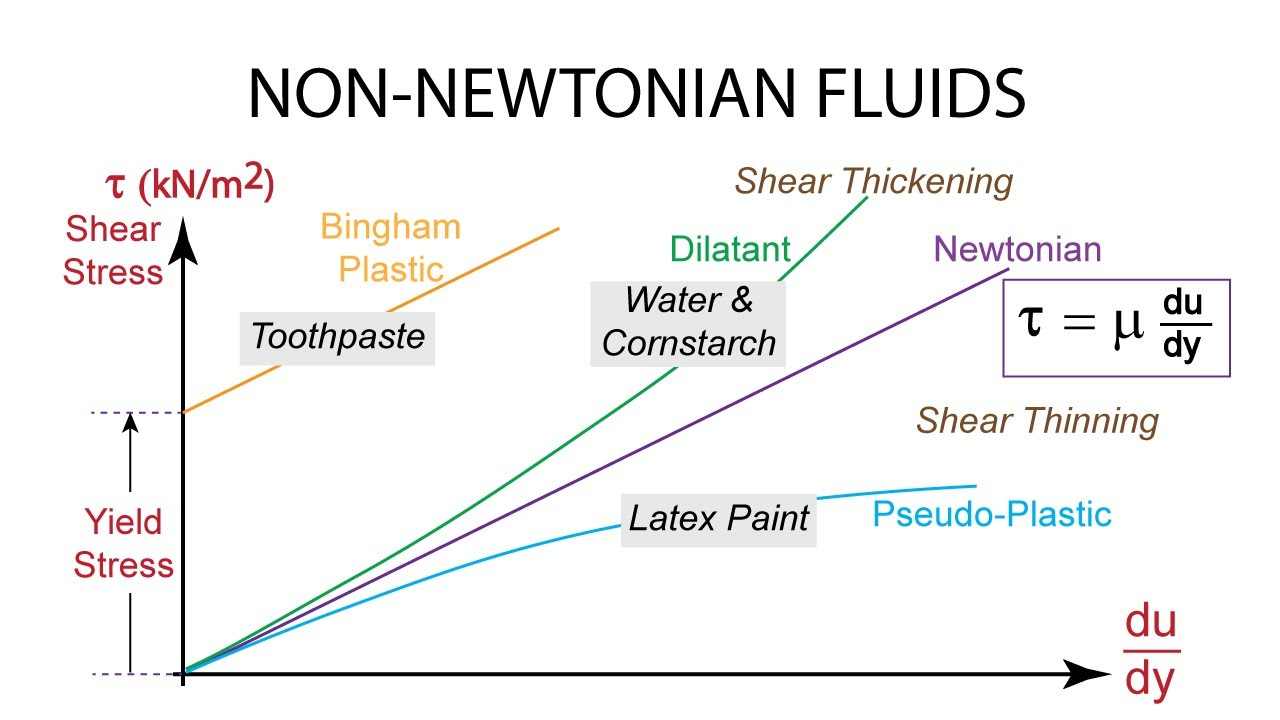
\includegraphics[width=8cm]{images/rheology/nnf}\\
{\captionfont no idea where this comes from ...}
\end{center}

%.....................................................................
\subsubsection{Power-law model \label{ss:powerlaw}} \index{general}{Power Law Rheology}

One of the simplest non-Newtonian viscosity model is the power law model, 
for which the viscosity depends on the (effective) deviatoric strain rate as follows:
\begin{equation}
\eta(\dot{\varepsilon}_e) = K \dot{\varepsilon}_{e}^{n-1}
\qquad \text{or } \qquad
\sigma = 2 K \dot{\varepsilon}_e ^n 
\end{equation}
where $n$ and $K$ are parameters. $n$ is called the power law index. $\dot{\varepsilon}_e$ 
is defined in  \eqref{eq:tauepse} and in the table here above. 
Note that a Newtonian viscosity is recovered when $n=1$. Also $n$ and $K$ may depend on temperature
(see Reddy  \cite[p339]{reddybook2}).

A so-called 'generalised' power law rheology is proposed in Iaffaldano \& bunge (2009) \cite{iabu09}:
\begin{equation}
\eta = K (\dot{\varepsilon}_{e}+\dot{\varepsilon}_0)^{n-1}
\end{equation}
so that in the rigid areas where $\dot{\varepsilon}_e \rightarrow 0$ the rheology 
uses instead a minimum strain rate value $\dot{\varepsilon}_0$.

\Literature: England \& Molnar (1997) \cite{enmo97}

%------------------------------
\subsubsection{Carreau model}
\index{general}{Carreau model} 

Note that this model is sometimes called Bird-Carreau in the literature. \index{general}{Bird-Carreau model}
As explained in Reddy \cite{reddybook2}, the power-law model poses no restriction on 
how small or large the viscosity may become, which may prove problematic once 
implemented as it can lead to runaway effects (strain rate becomes large $\rightarrow$
viscosity becomes smaller $\rightarrow$ strain rate becomes larger, etc ...).
This problem is alleviated in the so-called Carreau
\footnote{\url{https://en.wikipedia.org/wiki/Carreau_fluid}} model \cite{carr72} 
(see for example Zinani \& Frey (2007) \cite{zifr07}). 
The viscosity is then given by
\begin{equation}
\eta(\dot{\varepsilon}_{e}) = \eta_\infty + (\eta_0-\eta_\infty) \left(1 + (\lambda \dot{\varepsilon}_{e})^2 \right)^{(n-1)/2}
\end{equation}
where $\eta_0$, $\eta_\infty$, $\lambda$ and $n\in[0,1]$ are material parameters. 
$\lambda$ is called the relaxation time: it is the inverse of the shear rate at which 
the fluid changes from Newtonian to power-law behavior.

At low strain rate a Carreau fluid behaves as a Newtonian fluid with viscosity $\eta_0$.
At intermediate strain rates $\dot{\varepsilon}_{e} \lambda \sim 1$ a Carreau fluid behaves 
as a Power-law fluid. At high strain rate, a Carreau fluid behaves as a Newtonian fluid 
again with viscosity $\eta_\infty$.
 
\begin{center}
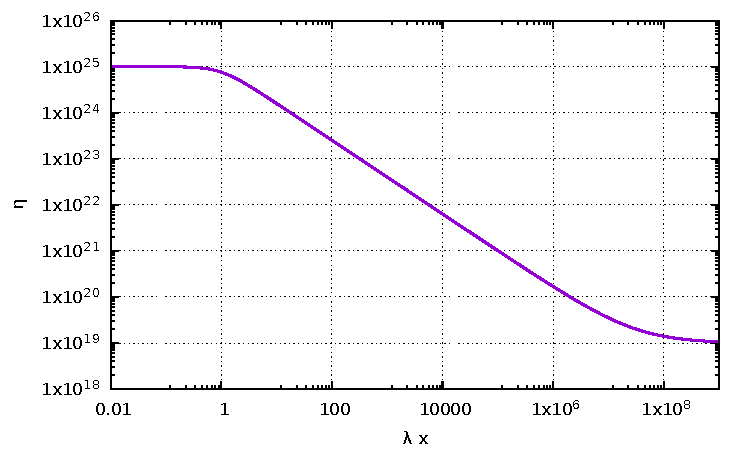
\includegraphics[width=7cm]{images/rheology/carreau/carreau.pdf}
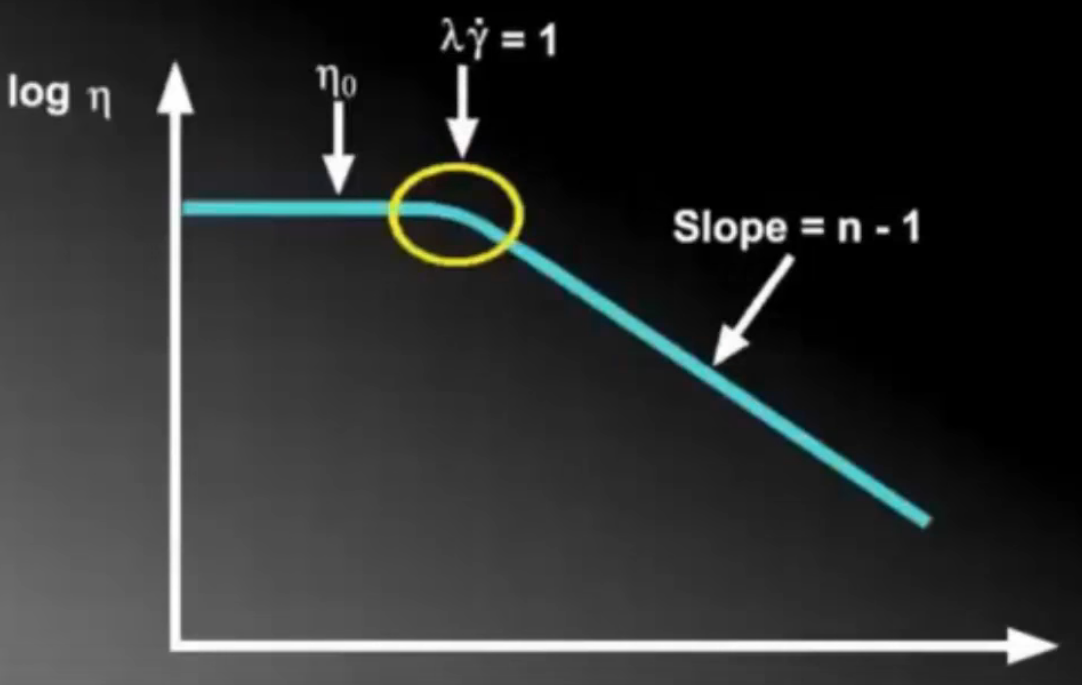
\includegraphics[width=6cm]{images/rheology/carreau/carreau1}\\
{\captionfont Left: Carreau model effective viscosity as a function of 
the product $\lambda \dot{\varepsilon}_{e}$. Right: taken from 
video at \url{https://youtu.be/qErs5zZV4BQ}.}
\end{center}

Note that the (Bird)-Carreau-Yasuda model \cite{yaac81,osru14} is very similar to the standard (Bird)-Carreau:
\begin{equation}
\eta = \eta_\infty + (\eta_0-\eta_\infty) \left(1 + (\lambda \dot{\varepsilon}_{e})^a \right)^{(n-1)/a}
\end{equation}
It is for instance used in van de Vosse \etal (2003) \cite{vadv03} to model blood.
\index{general}{Bird-Carreau-Yasuda model}

Flows in a Lid-Driven Cavity with this rheology are presented in \cite{zifr07,shal09}.

\Literature: Bercovici (1993) \cite{berc93}, Bercovici (1995) \cite{berc95},
Marcotte (2000) \cite{marc00}, Huerta \& Liu (1988) \cite{huli88}.

%------------------------------
\subsubsection{Bingham model} \label{sec:bingham}
\index{general}{Bingham model}

Bingham \cite{bingham} fluids can sustain an applied stress without any motion occuring. Only when the applied stress exceeds
a yield stress $\tau_0$ then the fluid flows. This translates as follows \cite{reddybook2}:

\begin{eqnarray}
{\bm \tau} &=& \left(  \frac{\tau_0}{\dot{\varepsilon}} + 2 \eta_0  \right)\dot{\bm \varepsilon}^d \qquad 
\text{ if } {\tau}_{e}>\tau_0 \\
{\bm \tau} &=& {\bm 0} \qquad\qquad\qquad\qquad  \text{if } \tau_{e} \leq \tau_0 
\end{eqnarray}
When flow occurs, the effective viscosity is then given by:
\begin{equation}
\eta(\dot{\varepsilon}_e) = \frac{\tau_0}{\dot{\varepsilon}_e} + 2 \eta_0 
\end{equation}
and when the strain rate is large we recover a Newtonian behaviour.
Typical Bingham fluids are mud, slurry, toothpaste.  

When using a velocity-based FEM code, the implementation of this rheological behaviour 
is complicated by the no-flow condition under a given stress. However, our codes
require a relationship between stress and strain rate in the form of an effective viscosity
which cannot be zero. 
This difficulty can be circumvented by implementing Bingham fluids as follows \cite{reddybook2}:

\begin{eqnarray}
{\bm \tau} &=& \left(  \frac{\tau_0(1-\eta/\eta_r)}{\dot{\varepsilon}_e} 
+ 2 \eta_0  \right)\dot{\bm \varepsilon} \qquad \text{ if } \tau_{e}>\tau_0 \\
{\bm \tau} &=& 2 \eta_r \dot{\bm \varepsilon}  \qquad\qquad\qquad\qquad\qquad\qquad  
\text{if } \tau_{e} \leq \tau_0 
\end{eqnarray}
where $\eta_r$ is a pre-yield viscosity and $\eta/\eta_r<<1$ (typically 1\% or less). This is a form of 
regularisation, and we will see a similar one in the next section.

Note the interesting paper by Barnes and Walter (1985) \cite{bawa85} who argue that 
"the yield stress concept is an idealization, and that, given accurate
measurements, no yield stress exists. The simple Cross model is shown to be a
useful empiricism for many non-Newtonian fluids, including those which have
hitherto been thought to possess a yield stress." The Cross model is presented 
in Section~\ref{ss:cross}.
 

\Literature: 
Papanastasiou (1987) \cite{papa87}, Blackery \& Mitsoulis (1997) \cite{blmi97},
Mitsoulis \& Zisis (2001) \cite{mizi01}, Mahmood \etal (2017) \cite{maky17},
Syrakos \etal (2014) \cite{syga14}, Bingham \cite{bingham}, Balmforth \& Rust (2009) \cite{baru09}, 
Grinevich \& Olshanskii (2009) \cite{grol09}, Sverdrup \etal (2018) \cite{svna18}
FE method for incompressible non-Newtonian flow (Bercovier \& Engelman (1980) \cite{been80});
Flow around a rigid sphere (Liu \etal (2002) \cite{limd02}),
Conduit flow of an incompressible, yield-stress fluid, \textcite{tawi97} (1997).

%------------------------------
\subsubsection{Herschel-Bulkley visco-plastic model}
\index{general}{Herschel-Bulkley model}

The Herschel-Bulkley model is effectively a combination of the power-law model and 
a simple plastic model:
\begin{eqnarray}
{\bm \tau} &=& 2 \left(  K \dot{\varepsilon}_e^{n-1} 
+ \frac{\tau_0}{\dot{\varepsilon}}\right)\dot{\bm \varepsilon} \qquad \text{ if } {\tau}_{e}>\tau_0 \\
\dot{\bm \varepsilon} &=& {\bm 0} \qquad\qquad \text{if }{\tau}_{e} \leq \tau_0 
\end{eqnarray}
in which $\tau_0$ is the yield stress, $K$ the consistency, and $n$ is the flow index \index{general}{Flow Index} \cite{demj04}.
The flow index measures the degree to which the fluid is shear-thinning ($n<1$) or shear-thickening ($n>1$).
If $n=1$ and $\tau_0=0$ the model reduces to the Newtonian model. 

The term between parenthesis above is the nonlinear effective viscosity. 
Concretely, the implementation goes as 
follows\footnote{\url{https://en.wikipedia.org/wiki/Herschel-Bulkley_fluid}}:
\begin{equation}
\eta(\dot{\bm \varepsilon}) = 
\left\{
\begin{array}{cc}
\eta_0 & \dot{\varepsilon}_e\leq \dot{\varepsilon}_0 \\ 
K \dot{\varepsilon}_e^{n-1} + \frac{\tau_0}{\dot{\varepsilon}_e} & \dot{\varepsilon}_e \geq \dot{\varepsilon}_0
\end{array}
\right.
\end{equation}
The limiting viscosity $\eta_0$ is chosen such that 
$\eta_0 =  K \dot{\varepsilon}_0^{n-1} + \frac{\tau_0}{\dot{\varepsilon}_0}$

A large limiting viscosity means that the fluid will only flow in response to a large applied force. 
This feature captures the Bingham-type behaviour of the fluid. 
Note that when strain rates are large, the power-law behavior dominates. 

As we have seen for Bingham fluids, the equations above are not easily amenable to implementation so that 
one usually resorts to regularisation, which is a modification of the 
equations by introducing a new material parameter which controls the exponential 
growth of stress. This way the equation is valid for both yielded 
and unyielded areas (Blackery \& Mitsoulis (1997) \cite{blmi97},
Papanastasiou (1987) \cite{papa87}, Zinani \& Frey (2007) \cite{zifr07}, 
Sverdrup \etal (2018) \cite{svna18}):
\begin{equation}
\eta(\dot{\varepsilon}_e) 
= K \dot{\varepsilon}_e^{n-1} + \frac{\tau_0}{\dot{\varepsilon}_e} [1 - \exp(-m \dot{\varepsilon}_e)] 
\end{equation}
When the strain rate becomes (very) small a Taylor expansion of the regularisation 
term yields $1- \exp(-m \dot{\varepsilon}) \sim m \dot{\varepsilon} $ so that 
$\eta_{eff} \rightarrow m \tau_0$.
However, it seems more physically meaningful to replace $m$ by a reference strain 
rate value $\dot{\varepsilon}_0$ so that 
\begin{mdframed}[backgroundcolor=blue!5]
\begin{equation}
\eta_{eff}(\dot{\bm \varepsilon}) 
= K \dot{\varepsilon}_e^{n-1} + \frac{\tau_0}{\dot{\varepsilon}_e} 
\left[1 - \exp\left(-\frac{\dot{\varepsilon}_e}{\dot{\varepsilon}_0} \right) \right]
\end{equation}
\end{mdframed}
In this case, when strain rate becomes (very) small a Taylor expansion of the regularisation
term yields
\begin{equation}
\frac{\tau_0}{\dot{\varepsilon}_e} \left[1 - 
\exp\left(-\frac{\dot{\varepsilon}_e}{\dot{\varepsilon}_0} \right) \right]
\simeq 
\frac{\tau_0}{\dot{\varepsilon}_e} \frac{\dot{\varepsilon}_e}{\dot{\varepsilon}_0}
=\frac{\tau_0}{\dot{\varepsilon}_0} 
\end{equation}
This has the dimensions of a viscosity and this is effectively the definition 
of a maximum viscosity $\eta_{max}$.

\noindent\Literature: 
\begin{itemize}
\item Viscous flow with large free surface motion (Huerta \& Liu (1988) \cite{huli88});
\item Numerical simulation of thermal plumes (Massmeyer \etal \cite{madd13}); 
\item Flows Through a Sudden Axisymmetric Expansion (Machado \etal \cite{mazf}, 
      Jay \etal (2001) \cite{jamp01}); 
\item Dam break problem (Ancey \& Cochard (2009) \cite{anco09}, 
      Cochard \& Ancey (2009) \cite{coan09}, Balmforth \etal \cite{bafp09};
\item Weakly compressible Poiseuille flow (Taliadorou (2009) \cite{tagm09});
\item Flow past cylinders in tubes (Mitsoulis \& Galazoulas (2009) \cite{miga09});
\item Determination of yield surfaces (Burgos \& Alexandrou (1999) \cite{buae99});
\item Carbopol hydrogel rheology for experimental
      tectonics and geodynamics (Di Giuseppe \etal (2015) \cite{dicf15}).
\item Flow past a sphere(disc) (Deglo de Besses \etal (2004) \cite{demj04}, 
      Gavrilov \etal (2017) \cite{gafp17}). \mscthesis\index{general}{MSc Thesis} 
\item Progress in numerical simulation of yield stress fluid flows, \textcite{sawa17} (2017) 
\end{itemize}


%...........................................................
\subsubsection{The Casson model}

It is described in Barnes (1999) \cite{barn99}:
\begin{equation}
\sqrt{\sigma} = \sqrt{\sigma_y} + \sqrt{\eta_p \dot{\varepsilon}_e} 
\end{equation}
or, when squaring it:
\begin{equation}
\sigma = \sigma_y + \eta_p \dot{\varepsilon}_e + 2\sqrt{\sigma_p \eta_p \dot{\varepsilon}_e} 
\end{equation}
This model has been found to accurately describe the behaviour of synthetic based muds \cite{adlo17}. 
See also Section~2.5.1 of \textcite{macosko}. 

%-------------------------------------------------
\subsubsection{The Ellis model\label{ss:ellis}}

An Ellis equation would be of the form \cite{robc01} 
\begin{equation}
\frac{\eta-\eta_\infty}{\eta_0-\eta_\infty} =
\frac{1}{1+(\sigma/\sigma_c)^m}
\end{equation}
where $\sigma$ is the shear stress, $\sigma_c$ is a critical shear stress
and $m$ is a large number. 
See also Section~2.4.3 of \textcite{macosko}. 

%-------------------------------------------------
\subsubsection{One model to rule them all? \label{ss:cross}}

Let us consider the base equation
\begin{equation}
\boxed{
\frac{\eta-\eta_\infty}{\eta_0-\eta_\infty} = 
\left[ 1+(K \dot{\varepsilon}_e)^a  \right]^{-(1-n)/a}
}
\end{equation}
This equation is purposefully generic and specific parameter combination choices 
allow to recover any of the above models (and more) \cite{osru14}.
See also an early paper by Cross (1965) \cite{cros65} for a somewhat similar equation.
See also Section~2.4.2 of \textcite{macosko}. 

%\begin{itemize}
%\item Newtonian:  $K=0$ is sufficient
%\item power-law: $\eta << \eta_0$, $\eta >> \eta_\infty$, $a=1$:
%\end{itemize}
Similar conclusions are reached in the following video:
\begin{center}
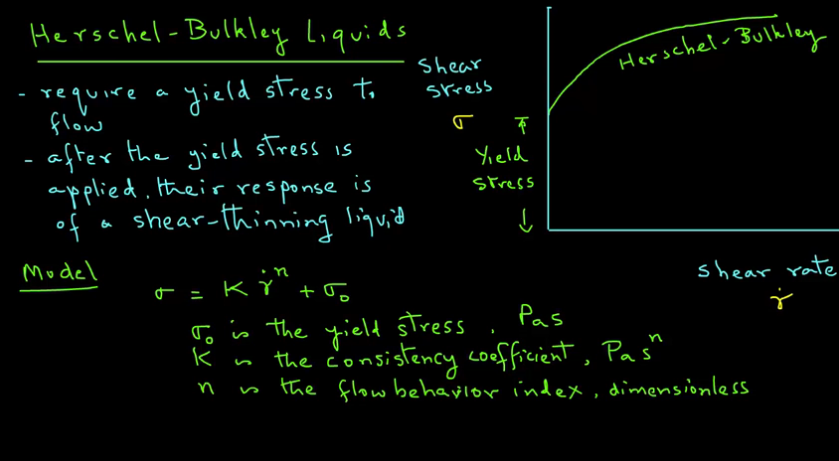
\includegraphics[width=7cm]{images/rheology/hbyoutube}\\
{\captionfont \url{https://youtu.be/dVCb11dZR7Y}}
\end{center}


\begin{center}
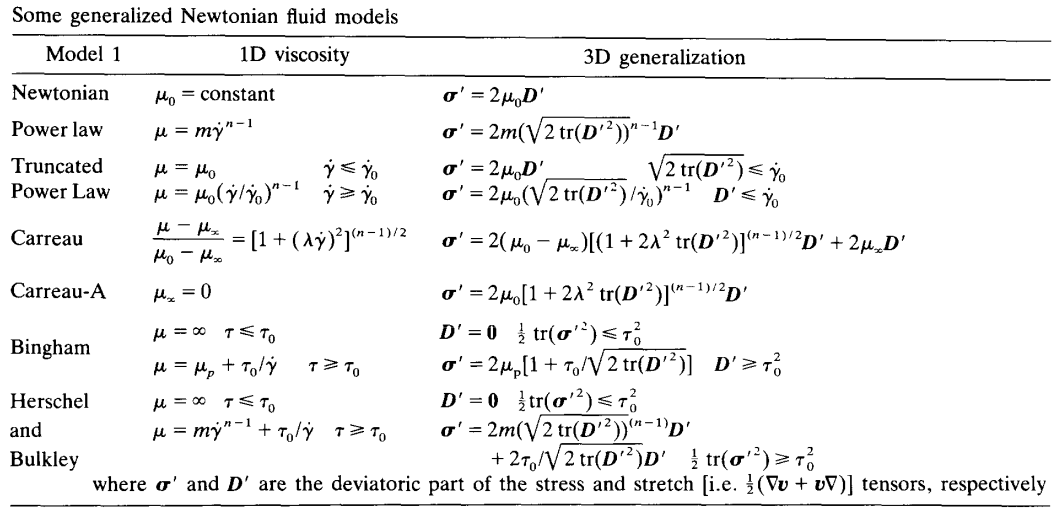
\includegraphics[width=7cm]{images/rheology/huli88}\\
{\captionfont Taken from \textcite{huli88} (1988)}
\end{center}


%-------------------------------------------------
\subsubsection{Dislocation and Diffusion creep}
\index{general}{Dislocation creep}
\index{general}{Diffusion creep}

\todo[inline]{insert here background and links to relevant textbooks}

The standard dislocation creep effective viscosity is given by:
\begin{mdframed}[backgroundcolor=blue!5]
\[
\eta^{ds}(p,T,\dot{\bm \varepsilon})
=\eta^{ds}(p,T,\dot{\varepsilon}_e)
= \frac{1}{2} f A^{-1/n} \dot{\varepsilon}_{e}^{(1-n)/n} \exp \left( \frac{Q+pV}{nRT}  \right)
\] 
\end{mdframed}
where $A$ is the pre-exponential scaling factor, $f$ is a scaling factor
representing viscous weakening or strengthening, $Q$ is the activation energy, 
$V$ is the activation volume, $T$ is the absolute temperature, $n$ is the power-law 
exponent, $R$ is the universal gas constant. 

The coefficients $A,n,Q,V$ are material parameters and are obtained in the laboratory 
by means of high pressure/temperature experiments (see for instance Karato \& Wu (1993) \cite{kawu93}). 
Unfortunately these experiments cannot be run at Earth-like strain rate 
values ($\sim 10^{-15}\si{\per\second}$)
so that extrapolations must be carried out over several orders of magnitude to 
arrive at values we can use in our numerical models. 
The 1/2 factor arises from the relationship between deviatoric stress and strain rate which 
involves a factor 2.

The factor $f$ is in fact a tuning parameter used to explore end members (e.g. 'weak crust' 
vs 'strong crust'), see discussion in the supplementary material in 
Huismans \& Beaumont (2011) \cite{hube11}. 
This approach has been extensively used by the \sopale users community, see 
for instance Warren \etal (2008) \cite{wabj08,wabj08b,wabj08c} 
or Gray \& Pysklywec (2012) \cite{grpy12}.

\todo[inline]{insert here equation for diffusion creep}

Furthermore, we know that several other factors will strongly affect the rheology:
\begin{itemize}
\item water content, or as often mentioned: 'dry' vs 'wet'. Following \cite{kawu93}, 
dry means water-free and wet means water-saturated conditions.
\begin{center}
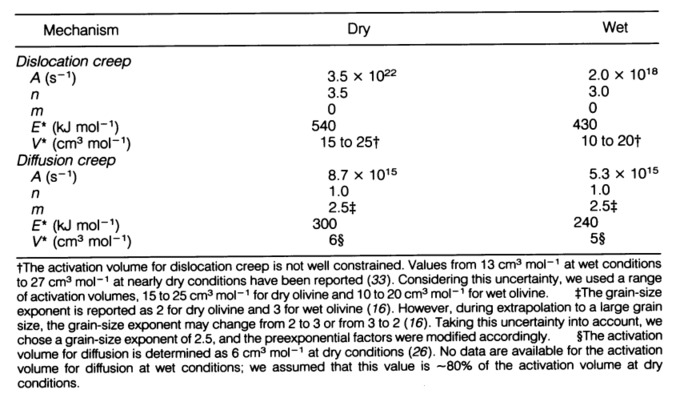
\includegraphics[width=8cm]{images/rheology/kawu93}\\
{\captionfont Taken from Karato and Wu \cite{kawu93}.}
\end{center}
\Literature: Quinquis \& Buiter (2014) \cite{qubu14} and refs therein for the effects of water
migration on models of subduction dynamics.

\item composition: while one typically assigns olivine properties to the mantle in models, 
the mineral olivine\footnote{\url{https://en.wikipedia.org/wiki/Olivine}} 
is actually a magnesium iron silicate with the formula (Mg$^{2+}$, Fe$^{2+}$)$_2$SiO$_4$.
and the ratio of magnesium to iron varies between the two endmembers of the solid solution series: 
forsterite (Mg-endmember: Mg$_2$SiO$_4$) and fayalite (Fe-endmember: Fe$_2$SiO$_4$).

\item grain size: this only affects diffusion creep mechanisms \cite{kawu93}. 
Grain size varies over several orders of magnitude and also evolves over time and 
its evolution is affected by the ambient deformation and the deformation history.
Dannberg \etal \cite{daef17} then used a diffusion creep effective viscosity 
given by:
\[
\eta^{df} = \frac{1}{2} A_{df}^{-1} d^m \exp \left( \frac{Q_{df}+pV_{df}}{RT}  \right)
\] 
where $d$ is the (variable) grain size and $m$ the grain size exponent. Grain growth/evolution 
is usually approximated using semi-empirical expressions \cite[section~2.2]{daef17}.
Smaller grains facilitating faster creep.

Relevant literature on this topic is in Section~\ref{sec:topics:gsev}.

\item anisotropy, LPO: see relevant literature in Section \ref{sec:topics:anisotropy}.

\item phase changes 
\end{itemize}

\begin{remark}
It is not uncommon to find in the literature effective viscosity formulations written as a function 
of $B$ with $B=A^{-1/n}$ \cite{wabj08,wabj08b,wabj08c}. Also, this $B$ coefficient often contains the conversion 
factor of the next remark.
\end{remark}

\begin{remark} Material parameters obtained in the lab are often measured on a uniaxial machine. 
An additional coefficient is added to the effective viscosity formula (see \cite{grpy12,grpy13}, 
or Table 1a of Warren \etal (2008) \cite{wabj08}):
$3^{-(1+n)/2n}2^{(1-n)/n}$. See page 77 of Ranalli \cite{ranalli} for an explanation.
\end{remark}

\begin{center}
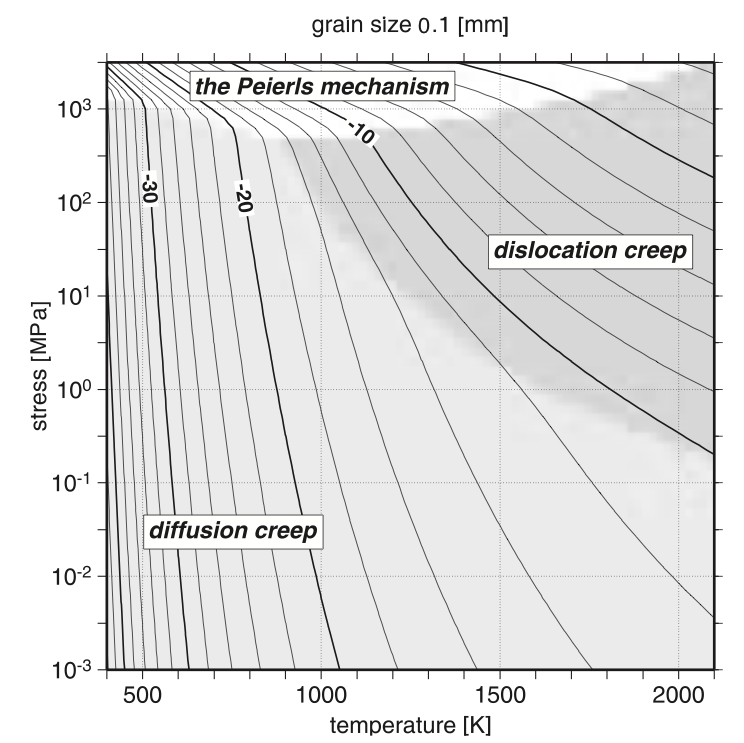
\includegraphics[width=7cm]{images/rheology/defmap}
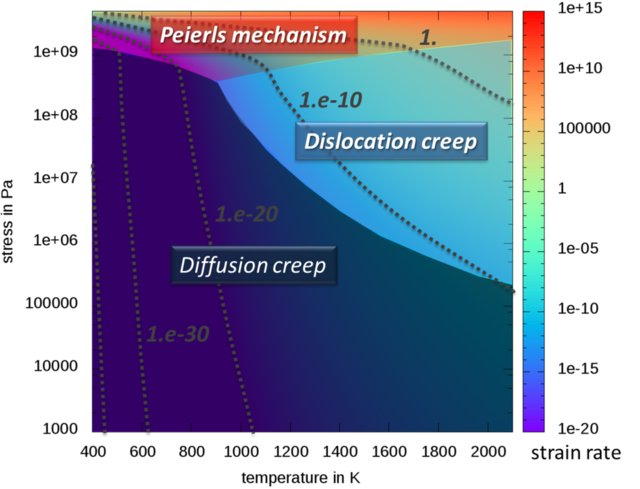
\includegraphics[width=9cm]{images/rheology/elme18}\\
{\captionfont 
Fig-$\mathds{B}$: Left: Taken from Kameyama \etal (1999) \cite{kayk99}.
Deformation mechanism map calculated for grain size $a=0.1\si{mm}$. The lightly shaded area indicates 
that deformation mainly occurs by diffusion creep. The densely shaded area indicates that 
deformation mainly occurs by power-law creep. 
The white region indicates that deformation mainly occurs by the Peierls mechanism. The 
solid curves are lines of constant strain rate. The numbers attached to each contour indicate the 
logarithm of the strain rate in the unit of $\si{\per\second}$.
Right: Taken from Elbeshausen \& Melosh (1998) \cite{elme18}. 
Strain rate as a function of stress and temperature. The parameter space dominated by each of 
the terms is denoted by different hues, depending on strain rate. Note that the original equations 
implicitly include a pressure dependence in the enthalpy term, which is not strong and 
therefore neglected here. The diffusion regime is highly temperature dependent and 
important for small strain rates only. Dislocation creep occurs for intermediate 
stresses and higher temperatures, while the Peierls mechanism dominates at higher stresses 
($\ge 500\si{\mega\pascal})$ and shows a strong stress dependence for low temperatures. 
The dashed contours are strain rate in units of $\si{\per\second}$. 
}
\end{center}


\paragraph{A closer look at the diffusion creep of Karato \& Wu (1993)} In the article, 
the following equation is used: 
\[
\dot{\bm \varepsilon} = 
A \left(\frac{{\bm \tau}}{\mu}\right) \left(\frac{b}{d}\right)^m \exp \left( -\frac{Q+pV}{RT}\right)
\]
where $\mu$ is the shear modulus ($\sim$80\si{\giga\pascal}), 
$b$ is the length of the Burgers vector ($\sim$0.5\si{\nano\metre}) and 
$d$ is the grain size.
One can express the above equation in terms of second invariants (see Section~\ref{sec:invariants}):
\[
\underline{\dot{\varepsilon}}_{e} 
= A \left(\frac{\underline{\tau}_{e}}{\mu}\right) \left(\frac{b}{d}\right)^m \exp\left( -\frac{Q+pV}{RT} \right)
\]
and assuming a Newtonian linearisation/relation between deviatoric stress 
and strain rate  $\underline{\tau}_{e} = 2 \eta^{df} \underline{\dot\epsilon}_{e}$, one arrive at
\[
\eta^{df} = \frac{1}{2} \left(\frac{A}{\mu}\right)^{-1}  
\left(\frac{b}{d}\right)^{-m} \exp\left( \frac{Q+pV}{RT} \right)
\]
or, 
\[
\eta^{df} = \frac{1}{2} \left[ \frac{A}{\mu}   
\left(\frac{b}{d}\right)^{m} \right]^{-1} \exp\left( \frac{Q+pV}{RT} \right)
\]
The effective diffusion creep viscosity is independent of strain-rate so that one 
could substitute the total pressure for lithostatic pressure in the equation, assume 
a geotherm and easily compute the predicted viscosity as a function of grain size $d$.

Let us assume that the 1D profile starts from the base of the lithosphere 
(say 120\si{\km} depth) and ends at the 660 boundary. 
Assume the temperature to increase linearly from 1300\degree C to $T_{bottom}$ (to 
be specified). At the bottom 
of the lithosphere, the lithostatic pressure is of the order of 
$\rho \cdot g \cdot L \simeq 3000\cdot 10 \cdot 120e3 \simeq 4$\si{\giga\pascal}. 
At the bottom of the domain, the pressure has increased 
by $3300\cdot 10 \cdot 630e3 \simeq21$\si{\giga\pascal}. 

The viscosity profile is plotted hereunder for three different grain sizes, bottom temperature and 
activation volumes (4,5,6 cm$^3$/mol). 

\begin{center}
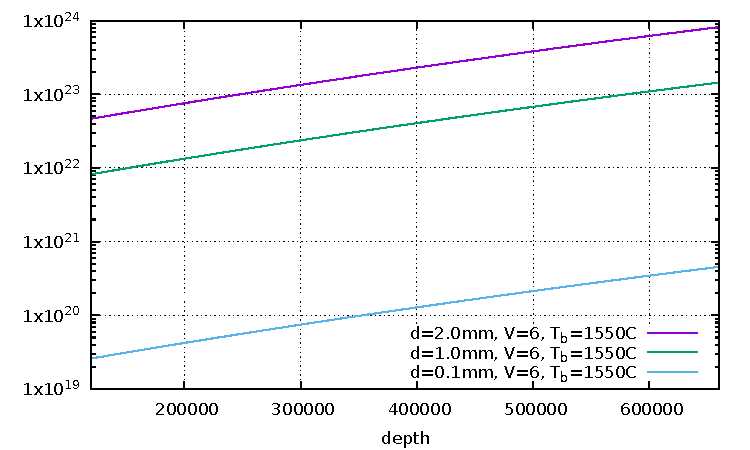
\includegraphics[width=5.cm]{images/rheology/kawudiff/viscosity1.pdf}
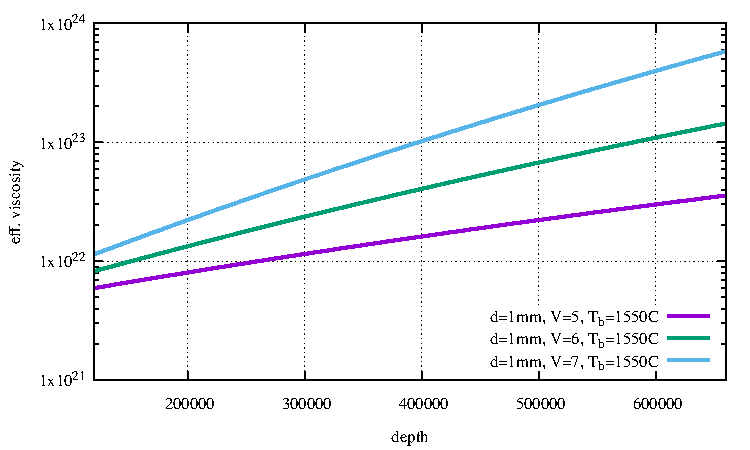
\includegraphics[width=5.cm]{images/rheology/kawudiff/viscosity2.pdf}
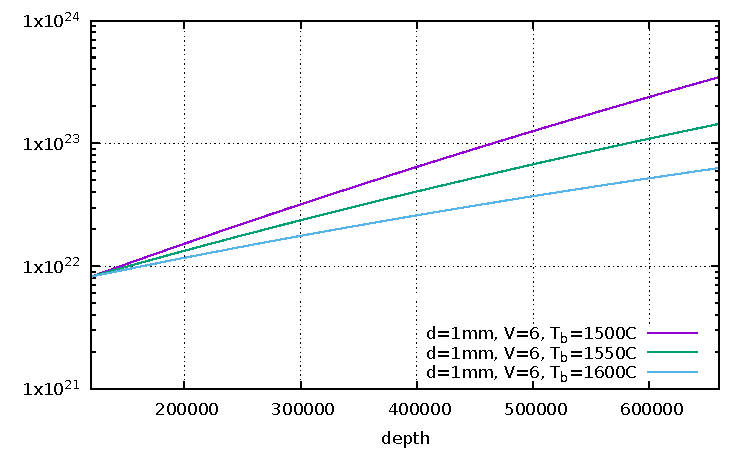
\includegraphics[width=5.cm]{images/rheology/kawudiff/viscosity3.pdf}\\
{\captionfont Effective diffusion creep viscosity for various 
grain size, activation volume and basal temperature values.}\\
{\color{gray} \tiny {images/rheology/kawudiff/}}
\end{center}

Although this exercise only provides us with first-order results, we can conclude that 
one can essentially change the diffusion creep effective viscosity by up to 2 orders of 
magnitude simply by choosing key parameters within acceptable ranges. 

\Literature: \textcite{didu18}\citetitle{didu18}

\newpage
%------------------------------
\subsubsection{The von Mises failure criterion}\label{sec:vMcriterion}
\index{general}{von Mises}
\begin{flushright} {\tiny {\color{gray} vMcriterion.tex}} \end{flushright}
%~~~~~~~~~~~~~~~~~~~~~~~~~~~~~~~~~~~~~~~~~~~~~~~~~~~~~~~~~~~~~~~~~~~~~~~~~~~~~~~~~~~~~~~~~~~~~~~~~~

The von Mises yield criterion suggests that the yielding of materials begins when the second 
deviatoric stress invariant ${\cal I}_2({\bm \tau})$ reaches a critical value. 
For this reason, it is sometimes called the $J_2$-plasticity or $J_2$ flow 
theory\footnote{$J_2$ is the common notation for ${\cal I}_2({\bm \tau})$}. 
It is part of a plasticity theory that applies best to ductile materials, such as metals. 

In material science and engineering the von Mises yield criterion can be also formulated in terms of 
the von Mises stress or equivalent tensile stress, $\sigma_v$, a scalar stress value that can be computed 
from the stress tensor. In this case, a material is said to start yielding when its von Mises stress 
reaches a critical value known as the yield strength, $\sigma_Y$. The von Mises stress is used to predict 
yielding of materials under any loading condition from results of simple uniaxial tensile tests. The 
von Mises stress satisfies the property that two stress states with equal distortion energy have equal 
von Mises stress. 

Because the von Mises yield criterion is independent of the first stress 
invariant, ${\cal I}_1({\bm \sigma})$, it is applicable 
for the analysis of plastic deformation for ductile materials such as metals, as the 
onset of yield for these materials does not depend on the hydrostatic component of the stress tensor. 

Although formulated by Maxwell in 1865, it is generally attributed to von Mises \cite{vonm13}. 
Huber (1904), in a paper in Polish, anticipated to some extent this criterion. 
Heinrich Hencky formulated the same criterion as von Mises independently in 1924 \cite{henc24,tata03}.
This criterion is also referred to as the Maxwell-Huber-Hencky-von Mises theory. 

The von Mises yield criterion (also known as Prandtl-Reuss yield criterion) 
is expressed in the principal stresses as
\[
\sqrt{{\cal I}_2({\bm \tau})} = c \quad \text{or}, \quad 
\frac{1}{6}[(\sigma_1 - \sigma_2)^2 + (\sigma_2 - \sigma_3)^2 + (\sigma_3 - \sigma_1)^2] =  c^2 
\]
where $c$ is the yield stress in uniaxial tension.
The von Mises yield criterion writes:

\begin{mdframed}[backgroundcolor=blue!5]
\begin{equation}
F^{\text{\tiny VM}}= \sqrt{{\cal I}_2({\bm \tau})  } - c  \label{vmcrit}
\end{equation}
\end{mdframed}
which is the Drucker-Prager criterion with $\phi=0$ (see Section~\ref{sec:dpcriterion}).

The following figure shows the von Mises yield surface in the three-dimensional space of principal stresses. 
\begin{center}
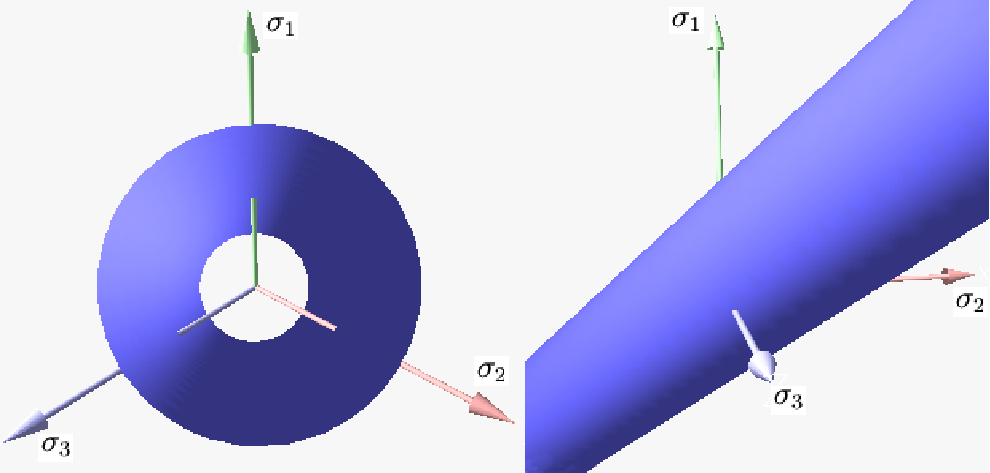
\includegraphics[width=0.6\textwidth]{images/rheology/vonmises/vonmises.pdf}\\
{\captionfont Most likely taken from Wikipedia...}
\end{center}
It is a circular cylinder of infinite length with its axis inclined at equal angles to the three principal stresses. 

\Literature: 
\fullcite{papa87}, \fullcite{ting03}

%\begin{center}
%\includegraphics[width=0.6\textwidth]{RHEOLOGY/viscoplasticity/vMcriterion.pdf}
%\end{center}
\paragraph{The yield surface} Let us try to draw the yield function in 
the space $\sigma_1,\sigma_2,\sigma_3$. It is given by
\begin{eqnarray}
&&\sqrt{ {\cal I}_2({\bm \tau}) } = c \\
&\Rightarrow&  {\cal I}_2({\bm \tau})  = c^2 \\
&\Rightarrow& \frac{1}{6}\left[(\sigma_{1}-\sigma_{2})^2 + (\sigma_{2}-\sigma_{3})^2 
+ (\sigma_{1}-\sigma_{3})^2 \right] =c^2 \\
&\Rightarrow & (\sigma_{1}-\sigma_{2})^2 + (\sigma_{2}-\sigma_{3})^2 + (\sigma_{1}-\sigma_{3})^2 = 6c^2 
\end{eqnarray}
or, temporarily setting $x=\sigma_1$, $y=\sigma_2$ and $z=\sigma_3$: 
\begin{eqnarray}
(x-y)^2 + (y-z)^2 + (x-z)^2 &=& 6c^2 \\
(x-y)^2 + y^2 - 2yz + z^2 + x^2 -2xz +z^2 &=& 6c^2\\
2z^2 - 2(x+y)z + (x-y)^2+x^2+y^2-6c^2 &=& 0
\end{eqnarray}
This is a second order polynomial in $z$. Its discriminant $\Delta$ is
\begin{eqnarray}
\Delta 
&=& 4(x+y)^2 - 4 \cdot 2 \cdot [(x-y)^2+x^2+y^2-6c^2] \nn\\
&=& 4x^2 + 8xy + 4y^2 - 8 [x^2-2xy+y^2 +x^2+y^2-6c^2] \nn\\
&=& 4x^2 + 8xy + 4y^2 - 8 [2x^2-2xy+2y^2 -6c^2] \nn\\
&=& 4x^2 + 8xy + 4y^2 - 16x^2+ 16xy -16y^2 +48 c^2 \nn\\
&=& -12x^2 + 24xy -12 y^2  +48 c^2 \nn\\
&=& -12(x^2 -2xy + y^2)  + 48 c^2 \nn\\
&=& -12(x-y)^2  + 48 c^2 \nn
\end{eqnarray}
Since I am looking for $z(x,y)\in \mathbb{R}$ then $\Delta >0$ and this 
imposes a restriction on admissible $x,y$ pairs:
\[
 -12(x-y)^2  + 48 c^2 \nn > 0
\]
\[
(x-y)^2  < 4 c^2 
\]
\[
x-y<2c   
\qquad
\text{or,}
\qquad
y-x<2c   
\]
\[
y> x-2c   
\qquad
\text{or,}
\qquad
y<x+2c
\]
So the discriminant is positive in the band given by $y>x-2c$ and $y<x+2c$ in the $x,y$-plane, 
which is a band centered around the line $y=x$.
When $\Delta>0$ we have then 
\[
z= \frac{2(x+y) \pm \sqrt{\Delta}}{4}
\]
which means that for each pair $x,y$ there are 2 $z$ values. 
The middle of this surface is given by the line $z=(x+y)/2$. 
The plane normal to this line is given by $z=-2(x+y)$.

This approach is reasonably simple for the von Mises criterion but 
quickly becomes intractable for other criteria.

\vspace{.5cm}

We now look into the derivatives of the von Mises plastic potential $Q^{\text{\tiny vM}}(\bm\sigma)$.
We have
\begin{equation}
Q^{\text{\tiny vM}}(\bm\sigma) =\sqrt{{\cal I}_2({\bm \tau})  } - c  
\end{equation}
Then
\begin{eqnarray}
\frac{\partial Q^{\text{\tiny vM}} }{\partial {\cal I}_1(\bm\sigma)} &=& 0 \\
\frac{\partial Q^{\text{\tiny vM}} }{\partial \sqrt{{\cal I}_2(\bm\tau)}}&=& 1 \\
\frac{\partial Q^{\text{\tiny vM}} }{\partial \theta_{\rm L}(\bm\tau)} &=& 0 
\end{eqnarray}
so 
\begin{eqnarray}
C_1^{\text{\tiny vM}} &=& 0  \\ 
C_2^{\text{\tiny vM}} 
&=& \frac{1}{2  \sqrt{{\cal I}_2(\bm\tau)}   } (1-0) 
= \frac{1}{2  \sqrt{{\cal I}_2(\bm\tau)}   } \\ 
C_3^{\text{\tiny vM}} &=& 0  
\end{eqnarray}


\newpage


%------------------------------
\subsubsection{The Tresca failure criterion}\label{sec:trcriterion}
\index{general}{Tresca}
The Tresca or maximum shear stress yield criterion is taken to be the work of Henri Tresca. It is also referred as the Tresca-Guest (TG) criterion. The functional form of this yield criterion is
\[
f(\sigma_1,\sigma_2,\sigma_3) = 0
\]
In terms of the principal stresses the Tresca criterion is expressed as
\[
{\max(|\sigma_1 - \sigma_2| , |\sigma_2 - \sigma_3| , |\sigma_3 - \sigma_1| ) = \sigma_0 }
\]
The following figure shows the Tresca-Guest yield surface in the three-dimensional space of principal stresses. 
\begin{center}
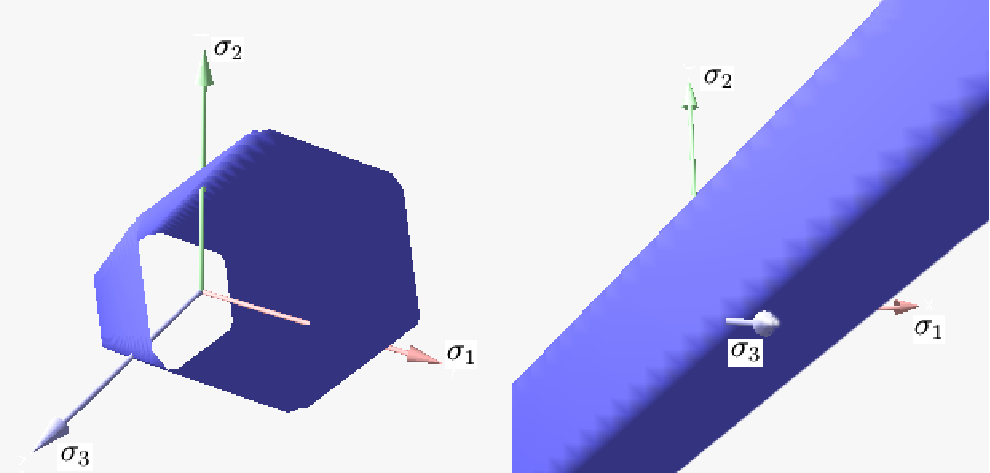
\includegraphics[width=0.6\textwidth]{images/rheology/tresca/Tresca.pdf}
\end{center}
It is a prism of six sides and having infinite length. This means that the material remains viscous when all three principal stresses are roughly equivalent (a hydrostatic pressure), no matter how much it is compressed or stretched. However, when one of principal stresses becomes smaller (or larger) than the others the material is subject to shearing. In such situations, if the shear stress reaches the yield limit then the material enters the plastic domain. 

\begin{remark}
The yield function is non-continuous, making its numerical implementation more difficult (directional derivatives are needed)
\end{remark}

%%%%%%%%%%%%%%%%%%%%%%%%%%%%%%%%%%
\paragraph{two-dimensional space}
Using the values of the principal stresses in a two dimensional space, the criterion becomes 
\[
|\sigma_1 - \sigma_2| =\sqrt{J_2'}  = \sigma_0 
\]
which is equivalent to the von Mises criterion.


%%%%%%%%%%%%%%%%%%%%%%%%%%%%%%%%%%
\paragraph{three-dimensional space}
We have already established that 
\begin{eqnarray}
\sigma_1 - \sigma_3  &=& 2 \sqrt{J_2} \cos \theta \nn
\end{eqnarray}
with $\sigma_1>\sigma_>\sigma_3$,
so that the failure criterion is given by

\begin{mdframed}[backgroundcolor=blue!5]
\[
F^{TR,3D}=2\sqrt{J_2}\cos \theta - c 
\]
\end{mdframed}

Obviously, the Tresca criterion corresponds to the case where the friction angle $\phi=0$.


\Literature: \cite{long03}


%------------------------------
\subsubsection{The Mohr-Coulomb failure criterion}\label{sec:mccriterion}
\index{general}{Mohr-Coulomb}
\begin{flushright} {\tiny {\color{gray} mccriterion.tex}} \end{flushright}
%~~~~~~~~~~~~~~~~~~~~~~~~~~~~~~~~~~~~~~~~~~~~~~~~~~~~~~~~~~~~~~~~~~~~~~~~~~~~~~~~~~~~~~~~~~~~~~~~~~

Mohr-Coulomb theory is a model describing the response of a material such as rubble piles or concrete to shear stress as well as normal stress. 
Most of the classical engineering materials somehow follow this rule in at least a portion of their shear failure envelope. In geology it is used to define shear strength of soils at different effective stresses \cite{hand69}.

In structural engineering it is used to determine failure load as well as the angle of fracture of a displacement fracture in concrete and similar materials. Coulomb's friction hypothesis is used to determine the combination of shear and normal stress that will cause a fracture of the material. Mohr's circle is used to determine the principal stresses that will produce this combination of shear and normal stress, and the angle of the plane in which this will occur. According to the principle of normality, the stress introduced at failure will be perpendicular to the line describing the fracture condition.

%It can be shown that a material failing according to Coulomb's friction hypothesis will show the displacement introduced at failure forming an angle to the line of fracture equal to the angle of friction. This makes the strength of the material determinable by comparing the external mechanical work introduced by the displacement and the external load with the internal mechanical work introduced by the strain and stress at the line of failure. By conservation of energy the sum of these must be zero and this will make it possible to calculate the failure load of the construction.

The Mohr-Coulomb failure criterion represents the linear envelope that is obtained from a plot of the shear strength of a material 
versus the applied normal stress. This relation is expressed as (Owen \& Hinton book \cite[p219]{owhi})
%\[
%\tau = c- \sigma~\tan(\phi) 
%\]

%Compression is assumed to be positive in the following discussion. If compression is assumed to be negative then $\sigma$ should be replaced with $-\sigma$.

%If $\phi=0$, the Mohr-Coulomb criterion reduces to the Tresca criterion. On the other hand, if $\phi = 90^\circ$ the Mohr-Coulomb model is equivalent to the Rankine model. Higher values of $\phi$ are not allowed.

\begin{equation}
\tau_m = -\sigma_m \sin \phi + c \cos \phi  \label{eq:mccrit}
\end{equation}
where $\tau_m$ is the magnitude of the shear stress, 
$\sigma_m$ is the normal stress, $c$ is the intercept of the failure envelope with the $\tau$ axis, 
and $\phi$ is the slope of the failure envelope.
The minus sign in the above equation is for the case where compression is assumed to be 
negative\footnote{\url{https://en.wikipedia.org/wiki/Mohr-Coulomb_theory}}.
The quantity $c$ is often called the cohesion and the angle $\phi$ is called the angle of internal friction.
 
We have  
\[
\tau_m=\frac{\sigma_1-\sigma_3}{2}
\qquad
\qquad
\sigma_m = \frac{\sigma_1+\sigma_3}{2}
\]
with $\sigma_1$ is the maximum principal stress and $\sigma_3$ is the minimum principal stress, or
%\[
%\sigma_1-\sigma_3 = - ( \sigma_1+\sigma_3) \sin \phi + 2c \cos \phi
%\]
%\[
%\sigma_1-\sigma_3 = 2 c \cos \phi - (\sigma_1+\sigma_3) \sin\phi
%\]
\begin{equation}
\cfrac{\sigma_1-\sigma_3}{2} = -\cfrac{\sigma_1+\sigma_3}{2}~\sin\phi +c\; \cos\phi 
\end{equation}
Using Eqs.~\eqref{eq:sig13a} and \eqref{eq:sig13b} 
for $(\sigma_1 - \sigma_3 )/2$ and $(\sigma_1 + \sigma_3 )/2$:
\begin{eqnarray}
&& \frac{\sigma_1 - \sigma_3}{2} = -\frac{\sigma_1 + \sigma_3}{2} \sin \phi  + c \cos \phi \nn\\
&\Rightarrow&
\sqrt{  {\cal I}_2({\bm \tau}) } \cos \theta = -\left(\frac{1}{3}{\cal I}_1({\bm \sigma}) - \sqrt{  {\cal I}_2({\bm \tau})} \frac{1}{\sqrt{3}} \sin \theta \right) \sin \phi 
+ c \cos \phi \nn\\
&\Rightarrow&
\frac{1}{3} {\cal I}_1({\bm \sigma}) \sin \phi  
+ \sqrt{  {\cal I}_2({\bm \tau}) } \left( \cos \theta - \frac{1}{\sqrt{3}} \sin \theta  \sin \phi \right) - c \cos \phi = 0 \nn
\end{eqnarray}

\begin{mdframed}[backgroundcolor=blue!5]
\begin{equation}
F^{\text{\tiny MC}}=\frac{1}{3} {\cal I}_1({\bm \sigma}) \sin \phi  + 
\sqrt{  {\cal I}_2({\bm \tau})  } \left( \cos \theta - \frac{1}{\sqrt{3}} \sin \theta  \sin \phi \right) - c \cos \phi
\label{eq:mcF} 
\end{equation}
\end{mdframed}
This formula (without the cohesion) is used in \textcite{will92}.
Since $p=-\frac{1}{3} {\cal I}_1({\bm \sigma})$, we also have:
%\begin{equation}
%F^{\text{\tiny MC}}= -p \sin \phi  + 
%\sqrt{ {\cal I}_2({\bm \tau})  } \left( \cos \theta - \frac{1}{\sqrt{3}} \sin \theta  \sin \phi \right) - c \cos \phi 
%\end{equation}
%or, 
\begin{mdframed}[backgroundcolor=blue!5]
\begin{equation}
F^{\text{\tiny MC}}=
\sqrt{  {\cal I}_2({\bm \tau})  } \left( \cos \theta - \frac{1}{\sqrt{3}} \sin \theta  \sin \phi \right) - (p \sin\phi + c \cos \phi)
\end{equation}
\end{mdframed}

\begin{remark}
The expression for $F$ in the Mohr-Coulomb case in Zienkiewicz \& Cormeau (1974) \cite{zico74} 
contains errors which are later corrected in \textcite[p102]{book_zitf}. 
\end{remark}

\Literature: this criterion is also used in computer graphics animation \cite{zhbr05}

\todo{when $\phi=0$ we should recover Tresca but factor 2 is wrong ?}



\vspace{.5cm}

We now look into the derivatives of the Drucker-Prager plastic potential $Q^{\text{\tiny MC}}(\bm\sigma)$.
We have
\[
Q^{\text{\tiny MC}}=
\frac{1}{3} {\cal I}_1({\bm \sigma}) \sin \phi  + 
\sqrt{  {\cal I}_2({\bm \tau})  } \left(\cos\theta_{\rm L}(\bm\tau)-\frac{1}{\sqrt{3}} 
\sin\theta_{\rm L} (\bm\tau) \sin\phi \right) -c \cos \phi
\]
Then
\begin{eqnarray}
\frac{\partial Q^{\text{\tiny MC}}  }{\partial {\cal I}_1(\bm\sigma)} &=& \frac13 \sin\phi \\
\frac{\partial Q^{\text{\tiny MC}}  }{\partial \sqrt {{\cal I}_2(\bm\tau)}}
&=&  
\cos \theta_{\rm L} - \frac{1}{\sqrt{3}} \sin \theta_{\rm L}  \sin \phi  
+  \sqrt{  {\cal I}_2({\bm \tau})  } 
\left(-\sin \theta_{\rm L} - \frac{1}{\sqrt{3}} \cos \theta_{\rm L}  \sin \phi \right) 
\frac{\partial \theta_{\rm L}}{\partial \sqrt {{\cal I}_2(\bm\tau)}   } \nn \\
&=&  
\cos \theta_{\rm L} - \frac{1}{\sqrt{3}} \sin \theta_{\rm L}  \sin \phi  
+  \sqrt{  {\cal I}_2({\bm \tau})  } 
\left(-\sin \theta_{\rm L} - \frac{1}{\sqrt{3}} \cos \theta_{\rm L}  \sin \phi \right) 
\frac{\partial \theta_{\rm L}}{\partial  {{\cal I}_2(\bm\tau)}   }  
\frac{\partial   {{\cal I}_2(\bm\tau)}     }{\partial \sqrt {{\cal I}_2(\bm\tau)}   }  \nn\\
&=&  
\cos \theta_{\rm L} - \frac{1}{\sqrt{3}} \sin \theta_{\rm L}  \sin \phi  
+  \sqrt{  {\cal I}_2({\bm \tau})  } 
\left(-\sin \theta_{\rm L} - \frac{1}{\sqrt{3}} \cos \theta_{\rm L}  \sin \phi \right) 
\left(
-\frac12 \tan 3\theta_{\rm L} \frac{1}{ {\cal I}_2(\bm\tau)} 
\right)
2 \sqrt {{\cal I}_2(\bm\tau)} \nn \\
&=&  
\cos \theta_{\rm L} - \frac{1}{\sqrt{3}} \sin \theta_{\rm L}  \sin \phi  
+  
\left(\sin \theta_{\rm L} + \frac{1}{\sqrt{3}}\cos\theta_{\rm L}\sin\phi\right) \tan 3\theta_{\rm L} \nn\\
&=&  
\cos \theta_{\rm L}
\left[
1 - \frac{1}{\sqrt{3}} \tan \theta_{\rm L}  \sin \phi  
+  
\left(\tan \theta_{\rm L} + \frac{1}{\sqrt{3}}   \sin \phi \right)  \tan 3\theta_{\rm L} 
\right] \nn\\
&=&
\cos \theta_{\rm L}
\left[
(1 +  \tan \theta_{\rm L}   \tan 3\theta_{\rm L})
+\frac{1}{\sqrt{3}} \sin\phi
( \tan 3\theta_{\rm L} - \tan\theta_{\rm L})
\right]
\\ 
\frac{\partial Q^{\text{\tiny MC}} }{\partial \theta_{\rm L}(\bm\tau)} 
&=&  
\sqrt{{\cal I}_2(\bm \tau)} (-\sin\theta_{\rm L}-\frac{1}{\sqrt{3}} \cos\theta_{\rm L} \sin\phi )\nn\\
&=&  
-\frac{1}{\sqrt{3}} \sqrt{{\cal I}_2(\bm \tau)} (\sqrt{3} \sin\theta_{\rm L}+\cos\theta_{\rm L} \sin\phi )
\end{eqnarray}
so
\begin{eqnarray}
C_1^{\text{\tiny MC}} &=& \frac13 \sin\phi  \\ 
C_2^{\text{\tiny MC}} 
&=& 
\frac{1}{2 \sqrt{ {\cal I}_2(\bm\tau)}   }   
\left( \frac{\partial Q}{\partial \sqrt{{\cal I}_2(\bm\tau)}} 
- \frac{\tan 3\theta_{\rm L}}{\sqrt {{\cal I}_2(\bm\tau)}}
\frac{\partial Q}{\partial \theta_{\rm L}(\bm\tau)}  
\right) \nn\\
&=& 
\frac{1}{2 \sqrt{ {\cal I}_2(\bm\tau)}   }   
\left( \cos \theta_{\rm L} \left[
(1 +  \tan \theta_{\rm L}   \tan 3\theta_{\rm L})
+\frac{1}{\sqrt{3}} \sin\phi ( \tan 3\theta_{\rm L} - \tan\theta_{\rm L}) \right]
+ \frac{\tan 3\theta_{\rm L}}{\sqrt {{\cal I}_2(\bm\tau)}}
\frac{1}{\sqrt{3}} \sqrt{{\cal I}_2(\bm \tau)} (\sqrt{3} \sin\theta_{\rm L}+\cos\theta_{\rm L} \sin\phi )
\right) \nn\\
&=& 
\frac{1}{2 \sqrt{ {\cal I}_2(\bm\tau)}   }   
\left( \cos \theta_{\rm L}
\left[ (1 +  \tan \theta_{\rm L}   \tan 3\theta_{\rm L})
+\frac{1}{\sqrt{3}} \sin\phi
( \tan 3\theta_{\rm L} - \tan\theta_{\rm L}) \right]
+ \tan 3\theta_{\rm L}  ( \sin\theta_{\rm L}+\frac{1}{\sqrt{3}}\cos\theta_{\rm L} \sin\phi )
\right) \nn\\
&=& 
\frac{1}{2 \sqrt{ {\cal I}_2(\bm\tau)}   }   
\left( \cos \theta_{\rm L} \left[
(1 +  \tan \theta_{\rm L}   \tan 3\theta_{\rm L})
+\frac{1}{\sqrt{3}} \sin\phi
( \tan 3\theta_{\rm L} - \tan\theta_{\rm L})
+ \tan 3\theta_{\rm L}   ( \tan\theta_{\rm L}+\frac{1}{\sqrt{3}} \sin\phi )
\right] \right) \nn\\
&=& 
\frac{1}{2 \sqrt{ {\cal I}_2(\bm\tau)}   }   
\cos \theta_{\rm L} \left[
(1 +  2\tan \theta_{\rm L}   \tan 3\theta_{\rm L})
+\frac{1}{\sqrt{3}} \sin\phi ( 2\tan 3\theta_{\rm L} - \tan\theta_{\rm L})
\right] \nn\\
C_3^{\text{\tiny MC}} 
&=&  - \frac{\sqrt{3}}{2\cos 3\theta_{\rm L}}
\frac{1}{{\cal I}_2(\bm\tau)^{3/2}} 
\frac{\partial Q}{\partial \theta_{\rm L}(\bm\tau)} \nn\\ 
&=&  - \frac{\sqrt{3}}{2\cos 3\theta_{\rm L}}
\frac{1}{{\cal I}_2(\bm\tau)^{3/2}} 
\left[-\frac{1}{\sqrt{3}} \sqrt{{\cal I}_2(\bm \tau)} (\sqrt{3} \sin\theta_{\rm L}+\cos\theta_{\rm L} 
\sin\phi ) \right]  \nn\\
&=&  \frac{\sqrt{3}\sin\theta_{\rm L} +  \sin \phi \cos \theta_{\rm L}}
{2 {\cal I}_2({\bm \tau}) \cos 3\theta_{\rm L}}
\end{eqnarray}










%\newpage
%\paragraph{two-dimensional space}

%The principal stress values are given by
%\[
%\sigma_{1,3} = \frac{\sigma_{xx}+\sigma_{yy}}{2} \pm \sqrt{ \frac{1}{4}(\sigma_{xx}-\sigma_{yy})^2 + \sigma_{xy}^2  }
%= \frac{J_1}{2} \pm \sqrt{ J_2'}
%\]
%so
%\[
%\frac{\sigma_1-\sigma_3}{2} = \frac{\sqrt{J_2}- - \sqrt{J_2}}{2} = \sqrt{J_2}
%\]
%\[
%\frac{\sigma_1+\sigma_3}{2} =  \frac{J_1}{2} 
%\]
%and then
%\[
%\sqrt{J_2} = - \frac{J_1}{2} \sin\phi + c\cos\phi 
%\]
%The Mohr-Coulomb criterion simply writes:
%
%\begin{mdframed}[backgroundcolor=blue!5]
%\begin{equation}
%F^{MC,2D}=  \frac{J_1}{2} \sin \phi + \sqrt{J_2} - c  \cos \phi  \label{mc2Dcriterion}
%\end{equation}
%\end{mdframed}

%%%%%%%%%%%%%%%%%%%%%%%%%%%%%%%%%%%%
%\paragraph{three-dimensional space}
%The Haigh-Westergaard invariants are related to the principal stresses by
%\begin{eqnarray}
%\sigma_1 &=& \cfrac{1}{\sqrt{3}}~\xi + \sqrt{\cfrac{2}{3}}~\rho~\cos\theta  \nonumber\\
%\sigma_3 &=& \cfrac{1}{\sqrt{3}}~\xi + \sqrt{\cfrac{2}{3}}~\rho~\cos\left(\theta+\cfrac{2\pi}{3}\right) \nonumber
%\end{eqnarray}
%Plugging into the expression for the Mohr-Coulomb yield function gives us
%\[
% -\sqrt{2}~\xi~\sin\phi + \rho[\cos\theta - \cos(\theta+2\pi/3)] - \rho\sin\phi[\cos\theta+\cos(\theta+2\pi/3)] = \sqrt{6}~c~\cos\phi 
%\]
%Using trigonometric identities for the sum and difference of cosines and rearrangement gives us the expression of the Mohr-Coulomb yield function in terms of $\xi$, $\rho$ and $\theta$:
%\[
%\left[\sqrt{3}~\sin\left(\theta+\cfrac{\pi}{3}\right) - \sin\phi\cos\left(\theta+\cfrac{\pi}{3}\right)\right]\rho - \sqrt{2}\sin(\phi)\xi = \sqrt{6} c \cos\phi 
%\]
%Alternatively, in terms of the invariants $p$,$q$,$r$ we can write
%\[
%\left[\cfrac{1}{\sqrt{3}~\cos\phi}~\sin\left(\theta+\cfrac{\pi}{3}\right) - \cfrac{1}{3}\tan\phi~\cos\left(\theta+\cfrac{\pi}{3}\right)\right]q - p~\tan\phi = c 
%\]

\newpage


%------------------------------
\subsubsection{The Drucker-Prager failure criterion \label{sec:dpcriterion}}
\index{general}{Drucker-Prager}
\begin{flushright} {\tiny {\color{gray} dpcriterion.tex}} \end{flushright}
%~~~~~~~~~~~~~~~~~~~~~~~~~~~~~~~~~~~~~~~~~~~~~~~~~~~~~~~~~~~~~~~~~~~~~~~~~~~~~~~~~~~~~~~~~~~~~~~~~~

The von Mises yield criterion is not suitable for modelling the yielding of frictional material 
as it does not include the effect of mean stress as observed in experiments. To overcome this 
limitation, Drucker and Prager (1952) \cite{drpr52} proposed a revised function for frictional materials.

The Drucker-Prager yield criterion has the function form
\begin{equation}
F^{\text{\tiny DP}}({\bm \sigma})=F \left( {\cal I}_1({\bm \sigma}), {\cal I}_2({\bm \tau}) \right) = 0 
\end{equation}
This criterion is most often used for concrete where both normal and shear stresses 
can determine failure. The Drucker-Prager yield criterion may be expressed as
\begin{mdframed}[backgroundcolor=blue!5]
\begin{equation}
F^{\text{\tiny DP}}= \sqrt{{\cal I}_2({\bm \tau})} + \alpha {\cal I}_1({\bm \sigma}) + k =0  
\label{dpcriterion} 
\end{equation}
\end{mdframed}
\todo[inline]{should it not be $-k$ ?}

\begin{center}
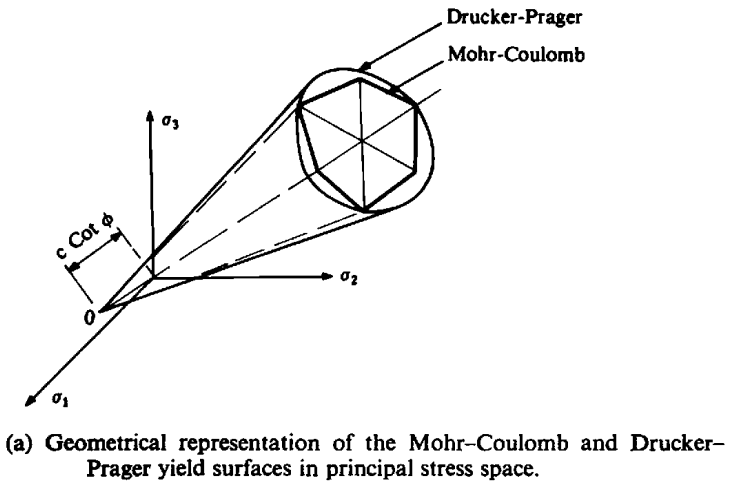
\includegraphics[width=6cm]{images/rheology/owenhinton5}\\
{\captionfont Taken from \textcite{owhi}.}
\end{center}

Using the parameters $\sigma_m$, $\tau_m$, $a=-\sqrt{3}\tan\theta$, ${\cal I}_1({\bm \sigma})$ 
and ${\cal I}_2({\bm \tau})$ of Section~\ref{sec:altinv} we have
\begin{eqnarray}
F^{\text{\tiny DP}}
&=&  \sqrt{{\cal I}_2({\bm \tau})} + \alpha {\cal I}_1({\bm \sigma}) + k \nn\\
&=& \sqrt{\frac{\tau_m^2}{3}(a^2+3)} + \alpha (3\sigma_m-a\tau_m) + k \nn\\ 
&=& \tau_m \sqrt{(a^2/3+1)} + \alpha (3\sigma_m+\tau_m\sqrt{3}\tan\theta ) + k    \qquad ({\rm since }\; \tau_m>0)\nn\\ 
&=& \tau_m \sqrt{\tan^2\theta+1} + \alpha (3\sigma_m+\tau_m\sqrt{3}\tan\theta ) + k  \nn\\
&=& \tau_m \sqrt{ \frac{1}{\cos^2\theta} } + \alpha (3\sigma_m+\tau_m\sqrt{3}\tan\theta ) + k  \nn\\
&=& \tau_m \frac{1}{\cos\theta} +\alpha (3\sigma_m+\tau_m\sqrt{3}\tan\theta ) + k  \qquad ({\rm since }\; \cos\theta >0)\nn
\end{eqnarray}
$F=0$ then leads to write
\begin{eqnarray}
\tau_m  + (3 \alpha \sigma_m+k)\cos\theta  + \tau_m \alpha \sqrt{3}\sin\theta  &=&0 \nn\\
\Rightarrow \qquad \tau_m(1 + \alpha \sqrt{3}\sin\theta)  + (3 \alpha \sigma_m+k)\cos\theta &=&0 \nn
\end{eqnarray}
and finally
\[
\tau_m = -\frac{(3 \alpha \sigma_m+k)\cos\theta}{1 + \alpha \sqrt{3}\sin\theta}
= -\frac{3 \alpha \cos\theta}{1 + \alpha \sqrt{3}\sin\theta} \sigma_m 
-\frac{k\cos\theta}{1 + \alpha \sqrt{3}\sin\theta}
\]
\begin{remark}
This is the same equation as Eq.~19 of Wojciechowski \cite{wojc18} but with $\theta \rightarrow -\theta$. 
\end{remark}

\vspace{.5cm}

The Mohr-Coulomb yield criterion writes  (see Eq.~\eqref{eq:mccrit})
\[
\tau_m = -\sigma_m \sin\phi + c \cos\phi
\]
so that equating both expressions of $\tau_m$ for the Drucker-Prager 
and Mohr-Coulomb criteria leads to:
\begin{eqnarray}
-\frac{3 \alpha \cos\theta}{1 + \alpha \sqrt{3}\sin\theta} &=& -\sin\phi \label{eq:qq1}\\
-\frac{k\cos\theta}{1 + \alpha \sqrt{3}\sin\theta} &=& c \cos\phi \label{eq:qq2}
\end{eqnarray}
Eq.~\eqref{eq:qq1} yields
\[
3 \alpha \cos\theta = \sin\phi (1 + \alpha \sqrt{3}\sin\theta) 
\]
\[
\Rightarrow \qquad 3 \alpha \cos\theta - \alpha \sqrt{3}\sin\theta \sin\phi = \sin\phi 
\]
and finally 
\[
\boxed{
\alpha(\phi) =  \frac{\sin\phi}{ 3 \cos\theta - \sqrt{3}\sin\theta \sin\phi}
}
\]
Inserting this into Eq.~\eqref{eq:qq2}:
\begin{eqnarray}
- k \cos\theta 
&=& c \cos \phi \left(1 +\alpha \sqrt{3} \sin\theta \right)  \nn\\
&=& c \cos \phi \left(1 + \frac{\sin\phi}{ 3 \cos\theta - \sqrt{3}\sin\theta \sin\phi}  \sqrt{3} \sin\theta\right) \nn\\
&=& c \cos \phi \left(1 + 
\frac{ \sqrt{3}\sin\phi \sin\theta }{ 3 \cos\theta - \sqrt{3}\sin\theta \sin\phi} \right) \nn\\
&=& c \cos \phi \left(
\frac{ 3 \cos\theta - \sqrt{3}\sin\theta \sin\phi}{ 3 \cos\theta - \sqrt{3}\sin\theta \sin\phi} 
+ 
\frac{ \sqrt{3}\sin\phi \sin\theta }{ 3 \cos\theta - \sqrt{3}\sin\theta \sin\phi} \right) \nn\\
&=& c \cos \phi \left(
\frac{ 3 \cos\theta}{ 3 \cos\theta - \sqrt{3}\sin\theta \sin\phi} \right) \nn
\end{eqnarray}
so that 
\[
\boxed{
k(c,\phi) =- \frac{ 3\; c \cos \phi }{ 3 \cos\theta - \sqrt{3}\sin\theta \sin\phi} 
}
\]
%Unsurprisingly we recover the Eqs. 20 and 21 of Wojciechowski \cite{wojc18} by replacing $\theta$ by $-\theta$.

The Drucker-Prager yield criterion which for a given $\theta$ is equal to the Mohr-Coulomb yield is then:
\begin{eqnarray}
F^{\text{\tiny DP}}
&=& \sqrt{{\cal I}_2({\bm \tau})} + \alpha(\phi) {\cal I}_1({\bm \sigma}) + k(c,\phi)  \nn\\
&=& \sqrt{{\cal I}_2({\bm \tau})} 
+ \frac{\sin\phi}{ 3 \cos\theta - \sqrt{3}\sin\theta \sin\phi}  {\cal I}_1({\bm \sigma})  
- \frac{ 3\; c \cos \phi }{ 3 \cos\theta - \sqrt{3}\sin\theta \sin\phi} \nn\\
&=& \sqrt{{\cal I}_2({\bm \tau})} 
- \left[ -\frac{3 \sin\phi}{ 3 \cos\theta - \sqrt{3}\sin\theta \sin\phi}  \frac{{\cal I}_1({\bm \sigma})}{3}
+ \frac{ 3\; c \cos \phi }{ 3 \cos\theta - \sqrt{3}\sin\theta \sin\phi} \right] \label{eq:Fdp}\\
&=& \sqrt{{\cal I}_2({\bm \tau})} 
- \left[ \frac{3\; p \sin\phi}{ 3 \cos\theta - \sqrt{3}\sin\theta \sin\phi} 
+ \frac{ 3\; c \cos \phi }{ 3 \cos\theta - \sqrt{3}\sin\theta \sin\phi} \right] \nn\\
&=& \sqrt{{\cal I}_2({\bm \tau})}  
- \frac{3\; p \sin\phi  + 3\; c \cos \phi }{ 3 \cos\theta - \sqrt{3}\sin\theta \sin\phi} \nn\\ 
&=& \sqrt{{\cal I}_2({\bm \tau})}  
- \frac{p \sin\phi  + c \cos \phi }{  \cos\theta - \frac{1}{\sqrt{3}}\sin\theta \sin\phi} 
\end{eqnarray}
which, when multiplied by $\cos\theta - \frac{1}{\sqrt{3}}\sin\theta \sin\phi$, gives
the Mohr-Coulomb criterion of Eq.~\eqref{eq:mcF}. 

For $\theta=\pi/6$, the DP yield surface {\bf circumscribes} the MC yield 
surface and Eq.~\eqref{eq:Fdp} writes:
\begin{eqnarray}
F^{\text{\tiny DP}}
&=& \sqrt{{\cal I}_2({\bm \tau})} 
- \left[ -\frac{3 \sin\phi}{ 3 \sqrt{3}/2 - \sqrt{3}/2 \; \sin\phi}  \frac{{\cal I}_1({\bm \sigma})}{3}
+ \frac{ 3\; c \cos \phi }{ 3 \sqrt{3}/2 - \sqrt{3}/2 \; \sin\phi} \right] \nn\\
&=& \sqrt{{\cal I}_2({\bm \tau})} 
- \left[ -\frac{6 \sin\phi}{\sqrt{3} (3 - \sin\phi) }  \frac{{\cal I}_1({\bm \sigma})}{3}
+ \frac{ 6\; c \cos \phi }{ \sqrt{3}(3 - \sin\phi)} \right] \nn\\
&=& \sqrt{{\cal I}_2({\bm \tau})} 
- \frac{ 6 p \sin \phi + 6\; c \cos \phi }{ \sqrt{3}(3 - \sin\phi)} \label{eq:dpc}
\end{eqnarray}
i.e.

\begin{center}
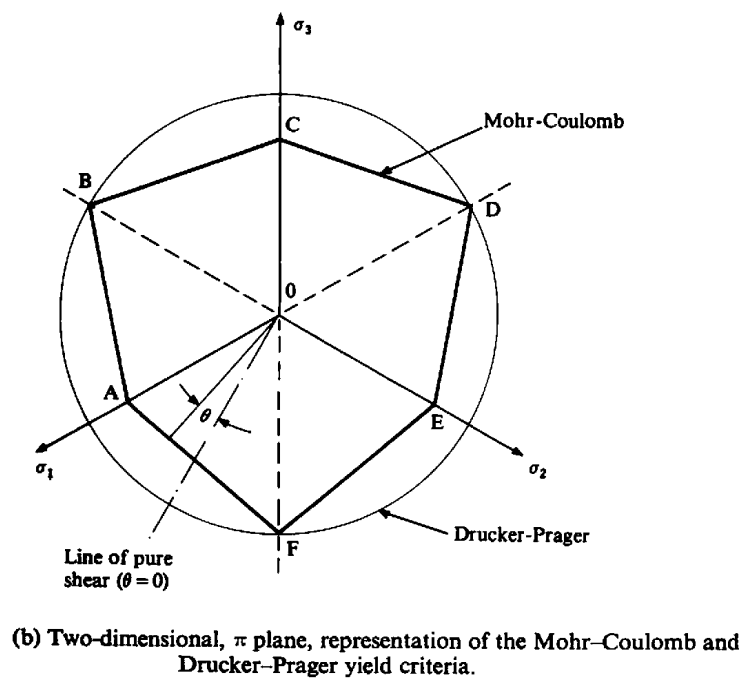
\includegraphics[width=5cm]{images/rheology/owenhinton6}\\
{\captionfont Taken from \textcite{owhi}.}
\end{center}

\begin{mdframed}[backgroundcolor=blue!5]
\begin{equation}
F^{\text{\tiny DP}}
= \sqrt{{\cal I}_2({\bm \tau})} 
+ \frac{ 6 \sin \phi }{ \sqrt{3}(3 - \sin\phi)} \frac{{\cal I}_1({\bm\sigma})}{3}
- \frac{ 6\; c \cos \phi }{ \sqrt{3}(3 - \sin\phi)} 
\end{equation}
\end{mdframed}

which is the formula used in Glerum \etal (2018) \cite{gltf18}.
This is also Eq.~(14a) in Zienkiewicz \& Cormeau (1974) \cite{zico74}, 
Eq.~(7.18) in \textcite{owhi}, and Eq.~(13.10a) in Zienkiewicz (1975) \cite{zien75} 
provided it is divided altogether by $\sqrt 3$. 


For $\theta=-\pi/6$, the DP yield surface {\bf middle circumscribes} the MC yield surface 
and Eq.~\eqref{eq:Fdp} writes:
\begin{eqnarray}
F^{\text{\tiny DP}}
&=& \sqrt{{\cal I}_2({\bm \tau})} 
- \left[ -\frac{3 \sin\phi}{ 3 \sqrt{3}/2 + \sqrt{3}/2 \sin\phi}  \frac{{\cal I}_1({\bm \sigma})}{3}
+ \frac{ 3\; c \cos \phi }{ 3 \sqrt{3}/2 + \sqrt{3}/2 \sin\phi} \right] \nn\\
&=& \sqrt{{\cal I}_2({\bm \tau})} 
- \left[ -\frac{6 \sin\phi}{\sqrt{3} (3 + \sin\phi) }  \frac{{\cal I}_1({\bm \sigma})}{3}
+ \frac{ 6\; c \cos \phi }{ \sqrt{3}(3 + \sin\phi}) \right] \nn\\
&=& \sqrt{{\cal I}_2({\bm \tau})} 
- \frac{6 p \sin\phi + 6 c \cos \phi}{\sqrt{3} (3 + \sin\phi) } 
\end{eqnarray}
This is Eq.~(7.19) of \textcite{owhi}.

Another DP formulation which {\bf inscribes} the MC yield surface is found on the 
wikipedia page of the Drucker-Prager yield criterion
\footnote{\url{https://en.wikipedia.org/wiki/Drucker-Prager_yield_criterion}}
(but I have no idea how it is arrived at):
\begin{eqnarray}
F^{\text{\tiny DP}}
&=& \sqrt{{\cal I}_2({\bm \tau})} 
- \left[ -\frac{3 \sin\phi}{\sqrt{9+3\sin^2\phi} }  \frac{{\cal I}_1({\bm \sigma})}{3}
+ \frac{ 3\; c \cos \phi }{ \sqrt{9+3\sin^2\phi} } \right] \label{eq:dp3}
\end{eqnarray}

The yield surfaces of these three Drucker-Prager formulations are plotted against the Mohr-Coulomb
yield surface in Section~\ref{ss:envelope}. 



%%%%%%%%%%%%%%%%%%%%%%%%%%%%%%%%%%
%\paragraph{two-dimensional space}

%By choosing $k=c \cos \phi $ and $\alpha=\frac{1}{2}\sin \phi$ and seeing that that $p=\frac{1}{2} {\cal I}_1({\bm \sigma})$, we can make the Drucker-Prager yield criterion coincide with the Mohr-Coulomb yield criterion
%so that 
%\begin{equation}
%F^{DP,2D} = \tau_e - (p \sin \phi + c \; \cos \phi) 
%\end{equation}


%%%%%%%%%%%%%%%%%%%%%%%%%%%%%%%%%%
%\paragraph{three-dimensional space}

%Let us first assume that the Drucker-Prager yield surface circumscribes the Mohr-Coulomb yield surface such that the two surfaces coincide at $\theta=\tfrac{\pi}{3}$. 
%The expression for the Mohr-Coulomb yield criterion is

%\[
%F^{MC,3D} = -\frac{1}{3}J_1 \sin \phi  + \sqrt{J_2} ( \cos \theta - \frac{1}{\sqrt{3}} \sin \theta  \sin \phi ) - c \cos \phi 
%\]
%Taking $\theta=\pi/6$ yields:
%\begin{eqnarray}
%F^{MC,3D} 
%&=& -\frac{1}{3}J_1 \sin \phi  + \sqrt{J_2} ( \frac{\sqrt{3}}{2} - \frac{1}{\sqrt{3}} \frac{1}{2}  \sin \phi ) - c \cos \phi  \nn\\
%&=& -\frac{1}{3}J_1 \sin \phi  + \frac{1}{2\sqrt{3}}\sqrt{J_2} ( 3 -  \sin \phi ) - c \cos \phi  \nn\\
%&=& -\frac{1}{3}J_1 \sin \phi  + \frac{1}{6}\sqrt{J_2} \sqrt{3}( 3 -  \sin \phi ) - c \cos \phi  \nn\\
%&=& \frac{\sqrt{3}(3-\sin\phi)}{6} \left( -  \frac{2 \sin \phi}{\sqrt{3}(3-\sin\phi)}   J_1  + \sqrt{J_2}  - \frac{6c \cos \phi}{\sqrt{3}(3-\sin\phi)} \right) \nn
%\end{eqnarray}
%The constant in front of the brackets (which always strictly positive) does not matter since we look at the sign of $F$.
%Comparing with 
%\[
%F^{DP}=\sqrt{J_2} - (\alpha J_1 + k) \label{dpcriterion} 
%\]
%we naturally set 
%\[
%\alpha =\frac{2 \sin \phi}{\sqrt{3}(3-\sin\phi)}
%\quad\quad\quad  
%k =  \frac{6c \cos \phi}{\sqrt{3}(3-\sin\phi)} 
%\]
%and since $p=\frac{1}{3}{\cal I}_1({\bm \sigma})$:
%\begin{mdframed}[backgroundcolor=blue!5]
%\begin{equation}
%F^{DP,3D} = \tau_e  - \left[ \frac{6 \sin \phi}{\sqrt{3}(3-\sin\phi)}   p  + 
%\frac{6c \cos \phi}{\sqrt{3}(3-\sin\phi)}  \right]
%\label{eqdp3D}
%\end{equation}
%\end{mdframed}
%\begin{center}
%\includegraphics[width=0.6\textwidth]{RHEOLOGY/viscoplasticity/dpcriterion.pdf}
%\end{center}


\vspace{1.3cm}
%..............
\begin{remark}
Leroy \& Ortiz \cite{leor89} use the Drucker-Prager plasticity model also and match it to the Mohr-Coulomb model in the 
triaxial test and formulate it as follows 
(Their definition of the second invariant of stress contains a 3/2 term):
\begin{eqnarray}
F 
&=& \tau_e \sqrt{3} + \frac{6 \sin\phi}{3-\sin\phi} \left( -p  - \frac{c}{\tan \phi} \right) \nn\\
&=& \tau_e \sqrt{3} - \left( \frac{6 \sin\phi}{3-\sin\phi}  p  + c \frac{6 \cos\phi}{3-\sin\phi} \right) \nn\\
&=& \sqrt{3} \left[ \tau_e  - \left( \frac{6 \sin\phi}{\sqrt{3}(3-\sin\phi)}  p  + c \frac{6 \cos\phi}{\sqrt{3}(3-\sin\phi)} \right)  \right]
\end{eqnarray}
Except for the $\sqrt{3}$ this is identical to Eq.~\eqref{eq:dpc}.
\end{remark}

%..............
\begin{remark}
Bui \etal (2008) \cite{bufs08} use yet again another formulation:
\begin{eqnarray}
F 
&=& \sqrt{{\cal I}_2({\bm \tau})} + \frac{\tan \phi}{\sqrt{9 + 12 \tan^2 \phi}} {\cal I}_1({\bm \sigma})
- \frac{3 c}{\sqrt{9 + 12 \tan^2 \phi}} \nn\\
&=& \sqrt{{\cal I}_2({\bm \tau})} + \frac{\sin \phi}{\sqrt{9\cos^2 \phi + 12 \sin^2 \phi}} {\cal I}_1({\bm \sigma}) - \frac{3 c \; \cos\phi}{\sqrt{9\cos^2\phi + 12 \sin^2 \phi}} \nn\\
&=& \sqrt{{\cal I}_2({\bm \tau})} + \frac{\sin \phi}{\sqrt{9 + 3 \sin^2 \phi}} {\cal I}_1({\bm \sigma}) - \frac{3 c \; \cos\phi}{\sqrt{9 + 3\sin^2 \phi}} \nn
\end{eqnarray}
which is identical to \eqref{eq:dp3}.
\end{remark}

%..............
\begin{remark}
Cacace \& Jacquey (2017) \cite{caja17} replace $\sqrt{{\cal I}_2({\bm \tau})}$ by 
$\sqrt{{\cal I}_2({\bm \tau})+\epsilon_0^2}$ where $\epsilon_0$ is a small non-hardening parameters 
here introduced to relax the singularity at the cone's tip of the Drucker-Prager yield envelope.
\end{remark}

\Literature:
\fullcite{cuwi14}


%.............................................................................
\paragraph{Dissecting the original paper by Drucker and Prager (1952)}


The authors state that a yield function which is a proper generalisation of the M-C hypothesis is:
\[
F = \alpha {\cal I}_1(\bm\sigma) + \sqrt{{\cal I}_2(\bm\tau)} - k
\]
where $\alpha$ and $k$ are positive constants at each point of the material.

According to the concept of plastic potential, the stress-train relation
corresponding to this yield function is 
\[
\dot\varepsilon_{ij}^{p} = \lambda \frac{\partial F}{\partial \sigma_{ij}}
\]
where $\dot\varepsilon_{ij}^{p}$ is the plastic strain rate and $\lambda$
is a positive factor of proportionality which may assume different values in space. Using the above expression for $F$:
\begin{equation}
\dot\varepsilon_{ij}^{p} = \lambda \left( \alpha \delta_{ij} + \frac{\tau_{ij}}{2\sqrt{{\cal I}_2(\bm\tau)}} \right)
\label{eq:dp52:ab}
\end{equation}
A very important feature of this equation is that the plastic rate of cubical
dilation is 
\begin{equation}
{\rm tr}[\dot{\bm \varepsilon}^{p}]
=\dot\varepsilon_{ii}^{p} = 3 \alpha \lambda \ne 0
\label{eq:dp52:bc}
\end{equation}
This equation shows that plastic deformation must be accompanied by an increase
in volume if $\alpha\ne 0$. This property is known as dilatancy.

%-----------------------------------------------------------------------
\paragraph{Plane strain} 
We need to establish three expressions.  
First, from Eq.~\eqref{eq:dp52:ab} we can write 
\[
\dot\varepsilon_{zz}^{p} = \lambda \left( \alpha  + \frac{\tau_{zz}}{2\sqrt{{\cal I}_2(\bm\tau)}} \right)
\]
but since $\dot\varepsilon_{zz}=0$ in plane strain then we find
\begin{equation}
\tau_{zz} = - 2 \alpha \sqrt{{\cal I}_2(\bm\tau)}
\end{equation}
which is Eq.~(6) of the paper. 

Second, we start from the definition of the first invariant and use the equation above:
\begin{eqnarray}
{\cal I}_1(\bm \sigma)&=& \sigma_{xx}+\sigma_{yy}+\sigma_{zz} \nn\\
{\cal I}_1(\bm \sigma)&=& \sigma_{xx}+\sigma_{yy}+\tau_{zz}+\frac13 {\cal I}_1(\bm \sigma) \nn\\
{\cal I}_1(\bm \sigma)&=& \sigma_{xx}+\sigma_{yy}- 2 \alpha \sqrt{{\cal I}_2(\bm\tau)} 
+\frac13 {\cal I}_1(\bm \sigma)\nn\\
\frac23 {\cal I}_1(\bm \sigma)&=& \sigma_{xx}+\sigma_{yy}- 2 \alpha \sqrt{{\cal I}_2(\bm\tau)} \nn\\
{\cal I}_1(\bm \sigma)&=& \frac32(\sigma_{xx}+\sigma_{yy})- 3 \alpha \sqrt{{\cal I}_2(\bm\tau)} 
\label{eq:I1dpps}
\end{eqnarray}
which is Eq.~(7) of the paper.

Finally, we start from (and we use the fact that $\sigma_{xx}-\sigma_{yy}=\tau_{xx}-\tau_{yy}$)
\begin{eqnarray}
\left(\frac{\sigma_{xx}-\sigma_{yy}}{2} \right)^2 + \tau_{xy}^2
&=& \frac14 \left(\sigma_{xx}-\sigma_{yy} \right)^2 + \tau_{xy}^2 \nn\\
&=& \frac14 \left(\sigma_{xx}-\sigma_{yy} \right)^2 
+ \underbrace{\tau_{xy}^2 
+ \frac12 (\tau_{xx}^2+\tau_{yy}^2+\tau_{zz}^2)}_{{\cal I}_2(\bm\tau)}
- \frac12 (\tau_{xx}^2+\tau_{yy}^2+\tau_{zz}^2) \nn\\
&=& \frac14 \left(\tau_{xx}-\tau_{yy} \right)^2 
+ {\cal I}_2(\bm\tau)
- \frac12 \tau_{xx}^2 -\frac12 \tau_{yy}^2 -\frac12 \tau_{zz}^2 \nn\\
&=& {\cal I}_2(\bm\tau) +\frac14\tau_{xx}^2 -\frac12\tau_{xx}\tau_{yy} +\frac14\tau_{yy}^2
- \frac12 \tau_{xx}^2 -\frac12\tau_{yy}^2 -\frac12 4\alpha^2 {\cal I}_2(\bm\tau) \nn\\
&=& {\cal I}_2(\bm\tau) -\frac14\tau_{xx}^2 -\frac12\tau_{xx}\tau_{yy} -\frac14\tau_{yy}^2
-2\alpha^2 {\cal I}_2(\bm\tau) \nn\\
&=& {\cal I}_2(\bm\tau) -\frac14(\tau_{xx}^2 +2\tau_{xx}\tau_{yy} +\tau_{yy}^2)
-2\alpha^2 {\cal I}_2(\bm\tau) \nn\\
&=& {\cal I}_2(\bm\tau) -\frac14(\underbrace{\tau_{xx}+\tau_{yy}}_{-\tau_{zz}})^2
-2\alpha^2 {\cal I}_2(\bm\tau) \nn\\
&=& {\cal I}_2(\bm\tau) -\frac14 \tau_{zz}^2 -2\alpha^2 {\cal I}_2(\bm\tau) \nn\\
&=& {\cal I}_2(\bm\tau) -\frac14 4\alpha^2 {\cal I}_2(\bm\tau) -2\alpha^2 {\cal I}_2(\bm\tau) \nn\\
&=& {\cal I}_2(\bm\tau) -3\alpha^2 {\cal I}_2(\bm\tau) \nn\\
&=& {\cal I}_2(\bm\tau)(1 -3\alpha^2)
\end{eqnarray}
so that 
\begin{equation}
{\cal I}_2(\bm\tau) = \frac{1}{1 -3\alpha^2} \left[\left(\frac{\sigma_{xx}-\sigma_{yy}}{2} \right)^2 + \tau_{xy}^2 \right]
\label{eq:dp52:cd}
\end{equation}
which is Eq.~(8) of the paper.

In the paper the authors propose the yield function 
\[
F = \alpha {\cal I}_1(\bm\sigma) + \sqrt{{\cal I}_2(\bm\tau)} - k
\]
We first replace the first (plane strain) invariant (see Eq.~\eqref{eq:I1dpps}):
\begin{eqnarray}
F 
&=& \alpha \left[ \frac32(\sigma_{xx}+\sigma_{yy})- 3 \alpha \sqrt{{\cal I}_2(\bm\tau)} \right]
+ \sqrt{{\cal I}_2(\bm\tau)} - k \nn\\
&=&\alpha \frac32(\sigma_{xx}+\sigma_{yy})- 3 \alpha^2 \sqrt{{\cal I}_2(\bm\tau)}
+ \sqrt{{\cal I}_2(\bm\tau)} - k  \nn\\
&=&\alpha \frac32(\sigma_{xx}+\sigma_{yy}) +(1- 3 \alpha^2) \sqrt{{\cal I}_2(\bm\tau)} - k \nn
\end{eqnarray}
and we now introduce the second invariant of Eq.~\eqref{eq:dp52:cd}:
\begin{eqnarray}
F &=& 
\alpha \frac32(\sigma_{xx}+\sigma_{yy}) +(1- 3 \alpha^2)
\frac{1}{(1 -3\alpha^2)^{1/2}} \left[\left(\frac{\sigma_{xx}-\sigma_{yy}}{2} \right)^2 
+ \tau_{xy}^2 \right]^{1/2} -  k  \nn\\
&=& \alpha \frac32(\sigma_{xx}+\sigma_{yy}) +(1- 3 \alpha^2)^{1/2}
\left[\left(\frac{\sigma_{xx}-\sigma_{yy}}{2} \right)^2 + \tau_{xy}^2 \right]^{1/2} 
- k  \nn\\
&=&\frac{3\alpha}{(1- 3 \alpha^2)^{1/2}}
\frac12(\sigma_{xx}+\sigma_{yy}) +
\left[\left(\frac{\sigma_{xx}-\sigma_{yy}}{2} \right)^2 + \tau_{xy}^2 \right]^{1/2} 
- \frac{k}{(1- 3 \alpha^2)^{1/2}} 
\nn\\
&=&\underbrace{\frac{3\alpha}{(1- 3 \alpha^2)^{1/2}}}_{\sin\phi}
\frac12(\sigma_{xx}+\sigma_{yy}) +
\left[\left(\frac{\sigma_{xx}-\sigma_{yy}}{2} \right)^2 + \tau_{xy}^2 \right]^{1/2} 
- \underbrace{\frac{k}{(1- 12 \alpha^2)^{1/2}}}_{c}
\underbrace{\frac{(1- 12 \alpha^2)^{1/2}}{(1- 3 \alpha^2)^{1/2}}}_{\cos\phi}
\end{eqnarray}


Note that if we define a triangle with sides $(1- 12 \alpha^2)^{1/2}$ and $3\alpha$
with hypotenuse $(1- 3 \alpha^2)^{1/2}$ then the angle $\phi$ makes sense and
we recover $\cos^2\phi+\sin^2\phi=1$.

In the end:
\[
F = 
\left[\left(\frac{\sigma_{xx}-\sigma_{yy}}{2} \right)^2 + \tau_{xy}^2 \right]^{1/2}
-\left(-\frac12(\sigma_{xx}+\sigma_{yy}) \sin \phi + c \cos \phi \right)
\]
which is the Mohr-Coulomb yield criterion of Eq.~(1) in the paper.


Note that when $\alpha=0$ (yield criterion independent of the mean stress - incompressible flow see Eq.~\eqref{eq:dp52:bc}) then $c=k$, $\cos\phi=1$ and $\sin\phi=0$ and we find 
the Tresca yield criterion
\[
F^{TR}=  \left[\left(\frac{\sigma_{xx}-\sigma_{yy}}{2} \right)^2 + \tau_{xy}^2 \right]^{1/2} - k
\]
Also, setting $\alpha=0$ in Eq.~\eqref{eq:dp52:cd} yields a criterion that writes
\[
F^{vM}={\cal I}_2(\bm\tau) - k
\]
which is the von Mises criterion! 



\vspace{.5cm}

We now look into the derivatives of the Drucker-Prager plastic potential $Q^{\text{\tiny DP}}(\bm\sigma)$.
We have
\[
Q^{\text{\tiny DP}} (\bm\sigma)= \sqrt{{\cal I}_2({\bm \tau})} + \alpha {\cal I}_1({\bm \sigma}) + k 
\]
Then
\begin{eqnarray}
\frac{\partial Q^{\text{\tiny DP}} }{\partial {\cal I}_1(\bm\sigma)} &=& \alpha \\
\frac{\partial Q^{\text{\tiny DP}} }{\partial \sqrt{{\cal I}_2(\bm\tau)}}&=& 1  \\
\frac{\partial Q^{\text{\tiny DP}} }{\partial \theta_{\rm L}(\bm\tau)} &=& 0 
\end{eqnarray}
The parameters $\alpha$ and $k$ can be expressed as a function of the angle of friction 
and cohesion so as to match the Mohr-Coulomb criterion in some sense (see above).
Then
\begin{eqnarray}
C_1^{\text{\tiny DP}} &=& \alpha  \\ 
C_2^{\text{\tiny DP}} &=& \frac{1}{2  \sqrt{{\cal I}_2(\bm\tau)}   }  \\ 
C_3^{\text{\tiny DP}} &=& 0  
\end{eqnarray}

ToDo: check \textcite{albo12} (2012) and compare with my notes above.









\newpage


%------------------------------
\subsubsection{The Griffith-Murrell failure criterion}
\index{general}{Griffith-Murrell}

The Griffith-Murrell yield criterion \cite{brau94,brbe95,babr97} is not often used. 
Extending the work of Griffith (1921) to three dimensional stress distributions, 
Murrell (1963) suggested the following criterion for rock failure expressed 
in terms of the principal stresses:
\[
(\sigma_1-\sigma_2)^2 + (\sigma_2-\sigma_3)^2 + (\sigma_3-\sigma_1)^2
+
24T_0 (\sigma_1+\sigma_2+\sigma_3)=0
\]
where $T_0$ is a material property called the tensile strength. In principal stress space, 
this criterion is represented by a paraboloid of revolution around the pressure (or hydrostatic) axis.

Using the definition of ${\cal I}_2({\bm \tau})$ and ${\cal I}_1({\bm \sigma})$, it also writes:
\[
{\cal I}_2({\bm \tau}) - 12 T_0 p =0
\]
which is the formulation used in Hansen \etal (2000) \cite{hanl00}, although the authors
use the lithostatic pressure instead of the full pressure. They also use a tensile 
strength parameter $T_0^e$ and a compressive strength parameter $T_0^c$, both around a few tens 
of MPas.

%------------------------------
\subsubsection{The Cam-clay failure criterion}
\index{general}{Cam-clay Failure Criterion}

\begin{flushright} {\tiny {\color{gray} camclay.tex}} \end{flushright}
%~~~~~~~~~~~~~~~~~~~~~~~~~~~~~~~~~~~~~~~~~~~~~~~~~~~~~~~~~~~~~~~~~~~~~~~~~~~~~~~~~~~~~~~~~~~~~~~~~~

The Original Cam-Clay model is based on the assumption that the soil 
is isotropic, elasto-plastic, deforms as a continuum, and it is not affected by creep.

\Literature: \cite{pehu03}

\todo[inline]{ask Chris Spiers. Pijnenburg et al, JGR 2019}



%.........................................................
\subsubsection{The failure envelope, or yield surface}
\label{ss:envelope} 

\Literature: Sch{\"o}pfer \etal (2013) \cite{sccm13}.

A yield surface is a five-dimensional surface in the six-dimensional space of stresses. 
The state of stress of inside the yield surface is elastic. 
When the stress state lies on the surface the material is said to have reached its yield point 
and the material is said to have become plastic. Further deformation of the material causes 
the stress state to remain on the yield surface, even though the surface itself may change shape and 
size as the plastic deformation evolves, this is because stress states that lie outside the yield surface are non-permissible.

The yield surface is usually expressed in terms of (and visualized in) a three-dimensional principal stress space $(\sigma_1,\sigma_2,\sigma_3)$, a two- or three-dimensional space spanned by stress invariants 
or a version of the three-dimensional Haigh-Westergaard space. 

\begin{center}
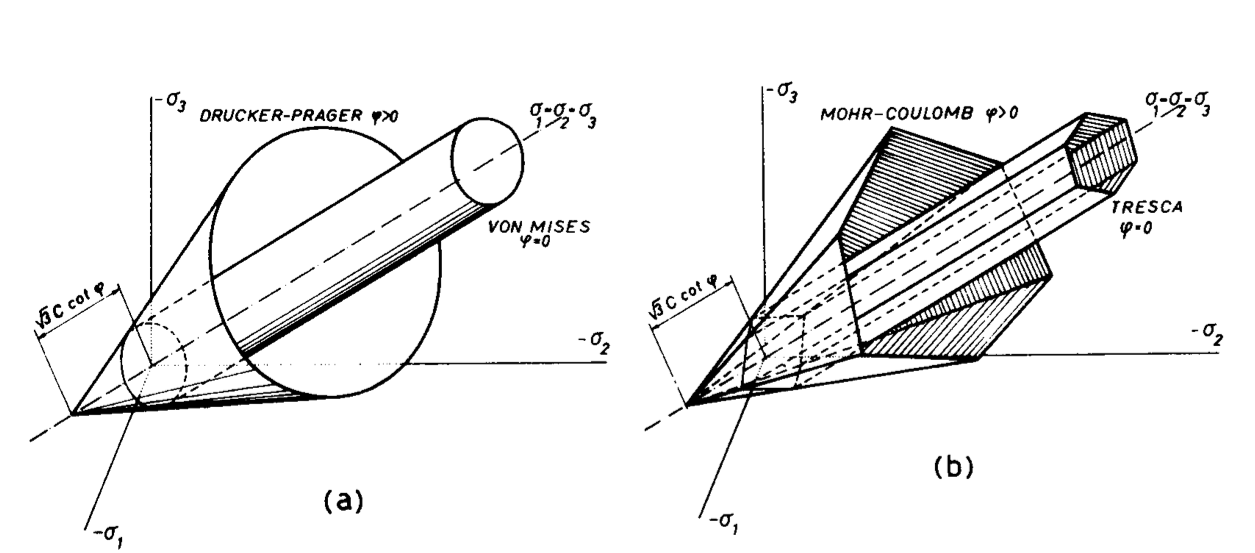
\includegraphics[width=14cm]{images/rheology/surfaces}\\
{\captionfont Yield surfaces in stress space \cite{zico74}. Note that 
the axes are $-\sigma_1$,$-\sigma_2$,$-\sigma_3$}
\end{center} 

Having obtained the equations for the yield functions in the previous sections, we can easily test
them as follows: in the ($\sigma_1$, $\sigma_2$, $\sigma_3$) space we can look for stress states 
that fulfil the yield equations. I set $c=20$MPa and $\phi=20$\degree and restrain 
the search to the space [-100MPa:100MPa]$^3$.
The python code and the gnuplot script used to generate the plots hereafter 
are in {\tt images/rheology/surfaces}. The implemented algorithm is somewhat  
naive and quite inefficient: discretise the space in $N^3$ points and for each point 
check whether any of the von Mises, Tresca, Mohr-Coulomb and (the three variants of) Drucker-Prager 
criteria is satisfied and when the point is in the space $\sigma_1+\sigma_2+\sigma_3=10$MPa 
(perpendicular to the $x=y=z$ line) write it to the corresponding file.

The recovered surfaces are similar to those of the figure above but their plot in a 3D space is difficult.
I have therefore isolated two sub-plots. 
The first one is for $\sigma_1=\sigma_2$:

\begin{center}
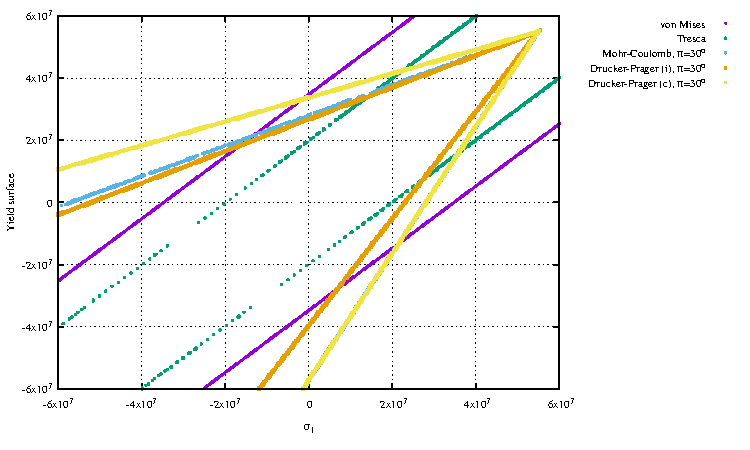
\includegraphics[width=12cm]{images/rheology/surfaces/surfaces_xy.pdf}
\end{center}
We see that the von Mises and Tresca envelopes are parallel to the line $\sigma_1=\sigma_2=\sigma_3$ (which 
is expected since they do not depend on pressure).

The second plot is in the plane $\sigma_1+\sigma_2+\sigma_3=0$ which is perpendicular to the middle line 
$\sigma_1=\sigma_2=\sigma_3=0$. To facilitate plotting the envelopes are plotted as a function of $\sigma_1$ only (so that even though they are circles in the chosen plane they appear here as ellipses):

\begin{center}
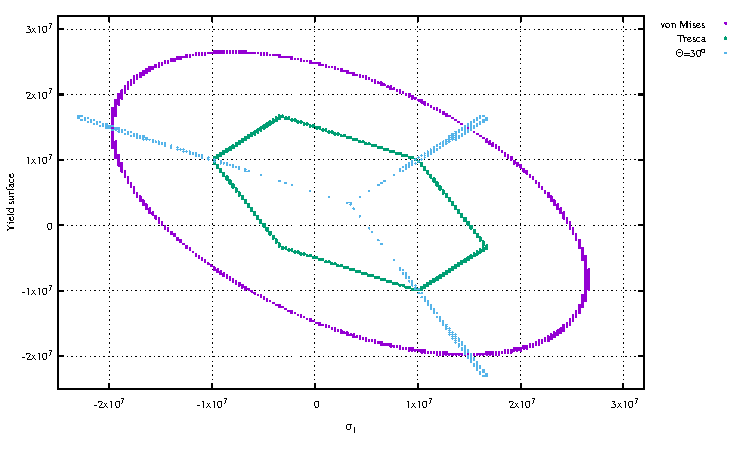
\includegraphics[width=12cm]{images/rheology/surfaces/surfaces_plane2.pdf}
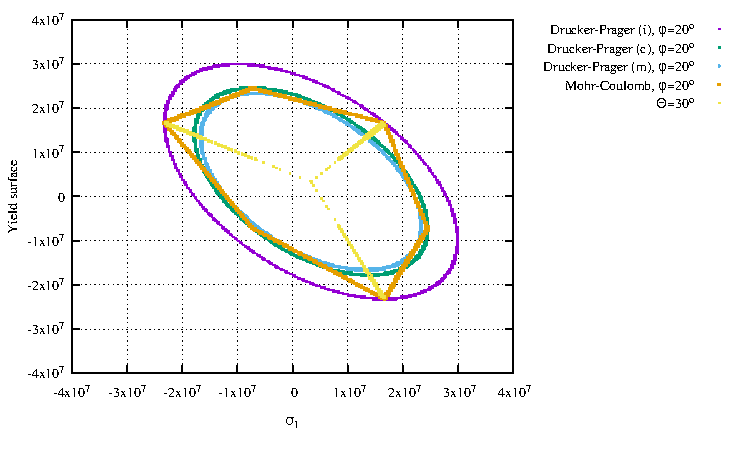
\includegraphics[width=12cm]{images/rheology/surfaces/surfaces_plane.pdf}
\end{center}

We see that we indeed recover that the three Drucker-Prager formulations 
inscribe (purple), middle-circumscribe (blue) and circumscribe (green) the 
Mohr-Coulomb one. 



\newpage
%------------------------------
\subsubsection{Peierls creep}
\index{general}{Peierls creep}
\begin{flushright} {\tiny {\color{gray} peierls.tex}} \end{flushright}
%~~~~~~~~~~~~~~~~~~~~~~~~~~~~~~~~~~~~~~~~~~~~~~~~~~~~~~~~~~~~~~~~~~~~~~~~~~~~~~~~~~~~~~~~~~~~~~~~~~

Looking at the literature, there seem to be many formulations for the Peierls creep deformation
mechanism, but it it appears that a standard formulation for the Peierls creep writes:
\[
\dot{\varepsilon} = A \sigma^n \exp \left[ -\frac{Q+pV}{RT} \left(1-(\frac{\sigma}{\sigma_P})^k\right)^q  \right]
\]
and it seems common to take $k=1$, and $n=2$ \cite{gery10,kaka08}
\[
\dot{\varepsilon} = A \sigma^2 \exp \left[ -\frac{Q+pV}{RT} \left(1-\frac{\sigma}{\sigma_P}\right)^q  \right]
\]
Elbeshausen \& Melosh (2018) \cite{elme18} use 
\[
\dot{\varepsilon} = A  \exp \left[ -\frac{Q}{RT} \left(1-\frac{\sigma}{\sigma_P}\right)^q  \right]
\]
In Chenin \etal (2019) \cite{chmd19} the authors state that their Peierls creep implementation
relies on parameters from Evans and Goetze (1979) \cite{evgo79} using the approach of 
Kameyama \etal (1999) \cite{kayk99}:
\[
\eta^{pe}=\frac{2}{3} \frac{(1-s)/s}{(1+s)/2s} A \; (\varepsilon_e^{ds})^{\frac{1}{n}-1} 
\]
with $A$ for this formulation:
\[
A = \left[ A_p \exp \left( -\frac{Q(1-\gamma)^2}{RT} \right)  \right]^{-1/s} \gamma \sigma_p
\]
where $s$ is an effective stress exponent that depends on the temperature:
\[
s = 2 \gamma \frac{Q}{RT} (1-\gamma)
\]
where $\gamma$ is a fitting parameter. 


\Literature 
\textcite{basv06},
\textcite{buro11},
\textcite{faff11},
\textcite{gagd14},
\textcite{gery10},
\textcite{goev79},
\textcite{kaka08},
\textcite{kako09},
\textcite{kary01},
\textcite{mesk10},
\textcite{zhwa13},
\textcite{chsm18},
\textcite{shwl17},
Review article from 1966: Guyot \& Dorn \cite{gudo67}





%-------------------------------------------------
\subsubsection{Stress limiting rheology}

Taken from van Hunen \etal (2002) \cite{vavv02}:
\[
\eta_y = \tau_y \dot{\varepsilon}_y^{-1/n_y} \dot{\varepsilon}_e^{(1/n_y) -1 } 
\]
where the yield stress $\tau_y$, the yield strain rate $\dot{\varepsilon}_y$ and the yield exponent $n_y$ are
prescribed parameters. In this article, $n_y=10$, $\dot{\varepsilon}_y=10^{-15}\si{\per\second}$
When $n_y=1$ the viscosity is constant and given by $\eta_{eff} = \tau_y / \dot{\epsilon}_y$.

This rheology has also been coined pseudo-plastic in Zhong \etal (1998) \cite{zhgm98}. 
Their equation is simply  
\[
\eta_{eff} = A^{1/n} \dot{\varepsilon}_e^{-1+1/n}
\]
where $A$ is the preexponent which depends on temperature, pressure, and composition.
\begin{center}
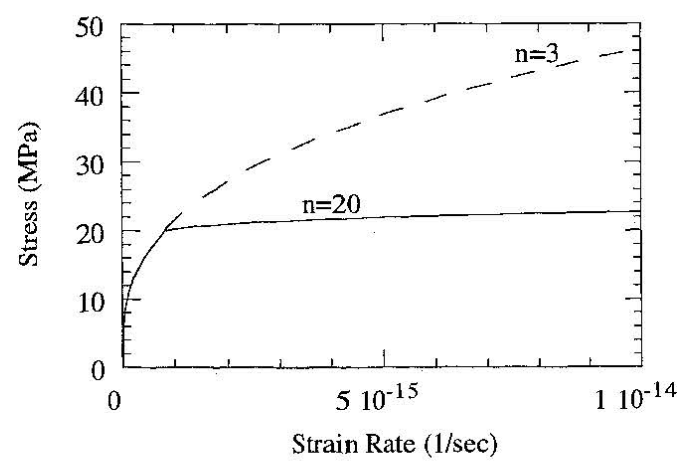
\includegraphics[width=5.5cm]{images/rheology/zhgm98}
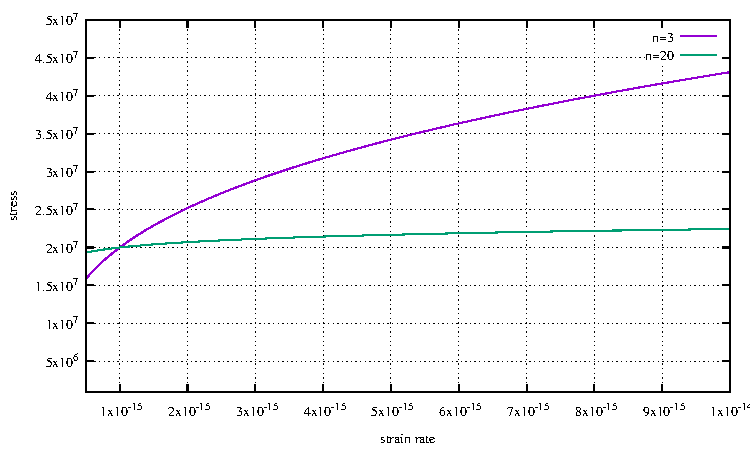
\includegraphics[width=5.8cm]{images/rheology/pseudoplastic/stress}
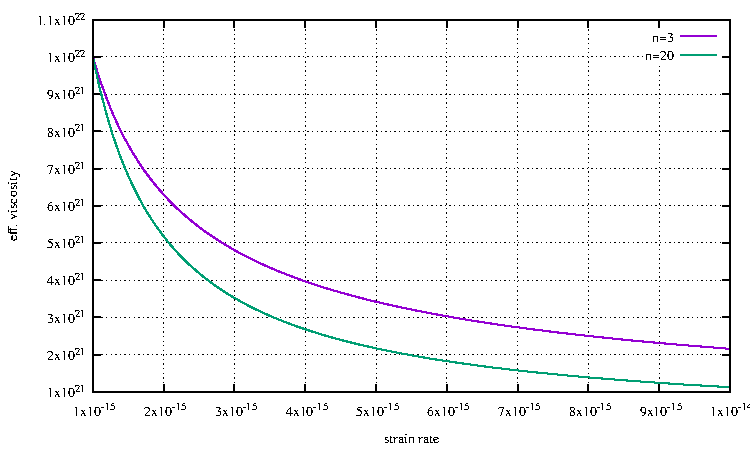
\includegraphics[width=5.8cm]{images/rheology/pseudoplastic/eta_eff}\\
{\captionfont Left figure is taken from \cite{zhgm98}. Authors report $A=7.9\cdot 10^{-8} \si{\pascal^3\second}$ 
for the $n=3$ case, which makes no sense. See gnuplot script for actual values of $A$.}
\end{center}




%-------------------------------------------------
\subsubsection{Arrhenius law}
\index{general}{Arrhenius law}

A purely temperature-dependent dimensional Arrhenius law that emulates the temperature
dependence of viscosity in silicate rock is often employed for mantle rocks 
\cite{albe00,zhzm09,vata11,bogs13b,namu13,stha13,boba19,gult19}:
\begin{equation}
\eta(T)=\eta_0 \exp \left( \frac{Q}{R}(\frac{1}{T}-\frac{1}{T_0}) \right)
\qquad 
{\rm or}
\qquad 
\eta(T)=\eta_0 \exp \left( \frac{Q}{RT} \right)
\end{equation}
where $\eta_0$ is a reference viscosity and $T_0$ its corresponding reference 
temperature.

It can also account for pressure effects as in \cite{lorg18} where the
diffusion creep viscosity (under the assumption of homogeneous grain size)
is temperature- and pressure-dependent:
\[
\eta(T)=\eta_0 \exp \left( \frac{1}{R}(\frac{Q-pV}{T}-\frac{Q}{T_0}) \right)
\]
(I find the minus sign rather suspicious)



%-------------------------------------------------
\subsubsection{Simple parametrisation of the mantle}

Many CITCOMs-based publications \cite{bumb10,budt14} 
have used the following (dimensionless) viscosity for the mantle:
\[
\eta(T,z) = \eta_r(r) \exp(A(0.5-T))
\]
where $\eta_r$ is a depth-dependent viscosity profile (usually defined as 
discontinuous linear profiles for various shells)

The non-dimensional activation coefficient is chosen to be $A=9.2103$ in 
\cite{budt14} which leads to a temperature-induced viscosity contrast of $10^4$ (for 
$T\in[0,1]$).

This is also called the Frank-Kamenetskii flow rule, as used in \cite{stha13,lemh17}:
\[
\eta' = \eta_0 \exp(-\theta T)
\]
where the the parameters $\eta_0$, $\theta$ account for the local chemical composition of the rock.
Note that the Frank-Kamenetskii approximation takes many forms in the literature \cite{nobr13}.
\index{general}{Frank-Kamenetskii}

Another temperature-dependent common expression is as follows \cite{flyu84}:
\[
\eta(T)=\eta_\infty \exp \left( \frac{Q}{R}(\frac{1}{T}-\frac{1}{T_\infty} ) \right)
\]
Also, following \cite{flyu84}: For studying transient convection in a non-
Newtonian rheological fluid, it is expedient from a
computational point of view to employ a law
which behaves linearly for low stresses initially
and becomes gradually non-Newtonian only after
a certain threshold stress level has been surpassed \cite{chri84,chyu84}:
\[
\eta(T,p,\tau_2) =\eta(T,p) \frac{1}{A_2 + A_3 \tau_2^2}
\]
where $A_2$ is a parameter describing the linear creep
at low stress levels and $A_3$ governs the transition
stress between Newtonian and non-Newtonian rheologies.

Coltice and Sheppard (2018) \cite{cosh18} use a depth- and temperature-dependent 
viscosity formulation:
\[
\eta(z,T)=\eta_0(z) \exp \frac{Q}{RT}
\]
Note that this expression is supplemented with a pseudo-plastic formulation \cite{roct12}.

\Literature: \cite{king16}

%-------------------------------------------------
\subsubsection{Glen's law for ice}\label{ss:glen}

As it turns out, ice and rocks share similarities in terms of rheology.
Glen's law is the most commonly used flow law for ice in glaciers and ice sheets \cite{glen55}
and it is actually a power-law type rheology:
\[
\dot{\bm \varepsilon} = A {\bm \tau}^n 
\]
with $n\sim 3$ and $A\sim 2.4\cdot 10^{-24} \text{Pa}^{-3}\cdot \text{s}^{-1}$ at $0\degree$C.
The effective viscosity is then given by
\[
\eta = \frac{1}{2 A \tau_e^{n-1}} 
\]
\begin{center}
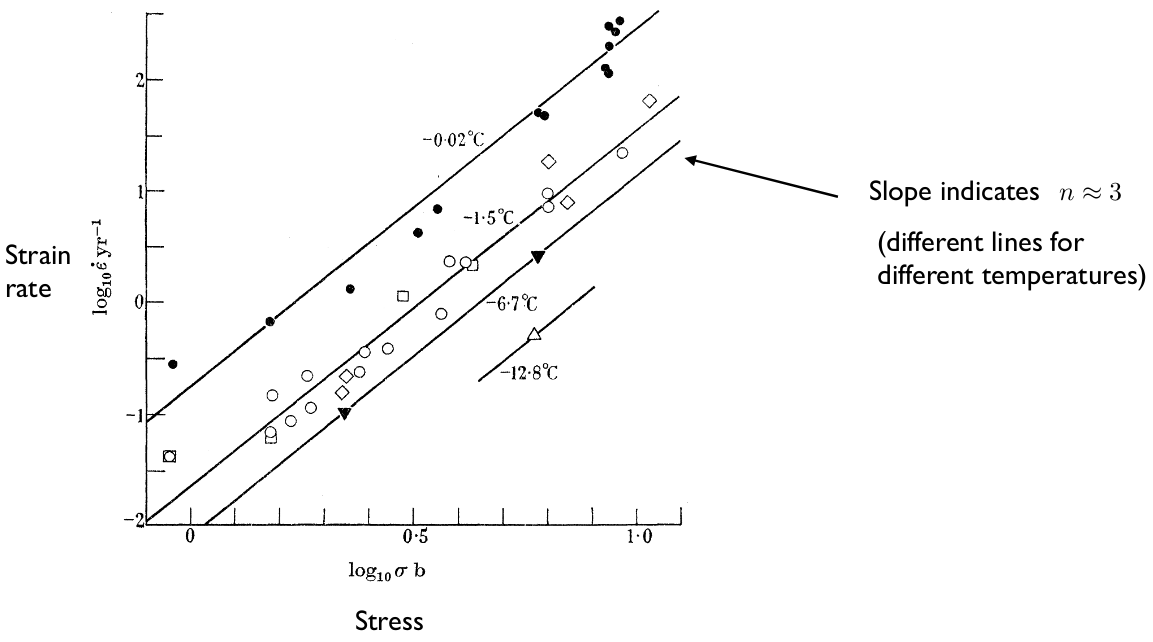
\includegraphics[height=5cm]{images/rheology/glen}
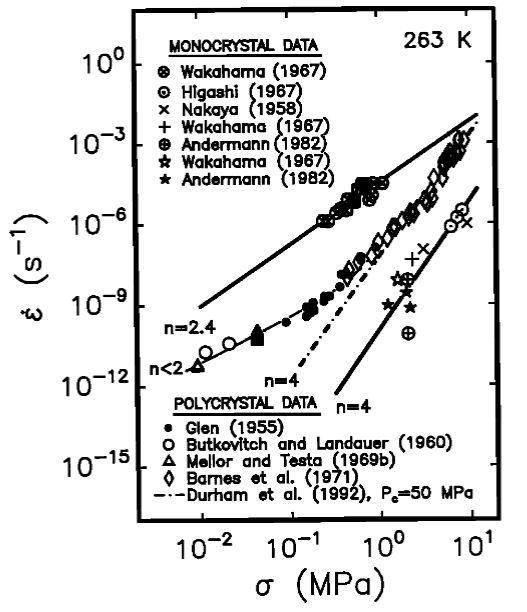
\includegraphics[height=5cm]{images/rheology/goko01}\\
{\captionfont Left: Taken from Glen \cite{glen55}; Right: taken from \cite{goko01}.}
\end{center}
Most of these studies suggest values of the power-law exponent $n\sim 2-4$, and there seems to be 
a general indication that the exponent is lower at lower stresses.

The $A$ coefficient above has been found to depend on temperature and is reasonably described 
with an Arrhenius law:
\[
A(T)=A_0 \exp\left( -\frac{Q}{RT} \right)
\]
A standard formulation is the Paterson-Budd law with a fixed Glen exponent $n=3$ and 
a split Arrhenius term \cite{pabu82}:
\[
A=3.615 \cdot 10^{-13} \text{Pa}^{-3}\cdot \text{s}^{-1}, \qquad Q=60 \; \text{kJ}/\text{mol}, \qquad if\quad T<263\text{K} 
\]
\[
A=1.733\cdot 10^{3} \text{Pa}^{-3}\cdot \text{s}^{-1}, \qquad  Q=139 \; \text{kJ}/\text{mol}, \qquad if\quad T>263\text{K}
\]
Be careful that in these two equations the temperature T is the pressure-adjusted temperature \cite{pabu82}.


Note that $A$ is also affected by the water content and the presence of impurities. 

Finally, Glen's law is the standard rheology used for ice-sheet modelling 
but it does not account for the complex evolution of fabric and resulting anisotropy.

\Literature \cite{grev97,krab16,grbl09,issg15,jidb17,heah18}. Very mathematics heavy papers: \cite{jora11,chgp13}.

%...........................................
\subsubsection{Strain rate partitioning across deformation mechanisms}\label{ss:srpart}
\index{general}{Strain rate partitioning}

When multiple viscous deformation mechanisms are present, one needs more dashpots, and 
more complicated element diagrams than the ones above occur (also when adding plastic deformation).
Two important rules are to be remembered:
1) for parallel components, stresses are additive, strain rates are equal in each; 
2) for components in series, stresses are equal in each and strain rates are additive. 

Let us then look at various assemblies of dashpots and plastic elements:

\begin{itemize}
\item \underline{two viscous dampers in series:} 

\begin{center}
\begin{tikzpicture}
%\draw[fill=gray!23,gray!23](0,0) rectangle (6,4.5);
%\draw[step=0.5cm,gray,very thin] (0,0) grid (6,4.5); %background grid

%left wall
\node[] at (0.1,2.7) {$\tau$};
\draw[line width=1mm] (0.5,1.5) -- (0.5,3.5) ;   
\draw [->] (0,2.5) -- (0.45,2.5);
\draw [->] (0,2) -- (0.45,2);
\draw [->] (0,3) -- (0.45,3);

%dashpots
\draw[thick] (0.5,2.5) -- (2,2.5) ;   
\draw[thick] (2.5,2.5) -- (4,2.5) ;   
\draw[thick] (4.5,2.5) -- (5.5,2.5) ;   
\draw[thick] (1.5,3) -- (2.5,3) -- (2.5,2) -- (1.5,2);  
\draw[thick] (3.5,3) -- (4.5,3) -- (4.5,2) -- (3.5,2);  

\node[] at (2,1.5) {$\eta_1$};
\node[] at (4,1.5) {$\eta_2$};

%wall
\draw[line width=2mm] (5.5,1.5) -- (5.5,3.5) ;   
\draw[thick] (5.5,1.5)  -- (5.75,1.75) ;   
\draw[thick] (5.5,1.75) -- (5.75,2) ;   
\draw[thick] (5.5,2)    -- (5.75,2.25) ;   
\draw[thick] (5.5,2.25) -- (5.75,2.5) ;   
\draw[thick] (5.5,2.5)  -- (5.75,2.75) ;   
\draw[thick] (5.5,2.75) -- (5.75,3) ;   
\draw[thick] (5.5,3)    -- (5.75,3.25) ;   
\draw[thick] (5.5,3.25) -- (5.75,3.5) ;

\draw[>=triangle 45, <->] (0.5,0.95) -- (3.,0.95);
\draw[>=triangle 45, <->] (3.,0.95) -- (5.5,0.95);
\node[] at (2,0.65)   {$\dot\varepsilon_{1}$};
\node[] at (4.25,0.65)   {$\dot\varepsilon_{2}$};

\end{tikzpicture}

\end{center}

each is subjected to the same stress $\tau$ but deforms 
with its own strain rate $\dot{\varepsilon}_1$ and $\dot{\varepsilon}_2$ and we have 
\begin{equation}
\dot{\varepsilon}_T 
= \dot{\varepsilon}_1 + \dot{\varepsilon}_2
= \frac{\tau}{2\eta_1} + \frac{\tau}{2\eta_2}
\end{equation}
The effective viscosity of this combination is denoted $\eta_{eff}$ and is such that 
$\eta_{eff}=\tau/2\dot{\varepsilon}_T$, which means that 
\[
\frac{\tau}{2\eta_{eff}} = \frac{\tau}{2\eta_1} + \frac{\tau}{2\eta_2}
\]
or, 
\[
\eta_{eff}= \left( \frac{1}{\eta_1} + \frac{1}{\eta_2} \right)^{-1}
\]
i.e. it follows that the effective viscosity of two or more viscous dampers in series is the harmonic 
average of the individual viscosities of the dampers.

In general, for n dampers in series:
\[
\eta_{eff}= \left( \sum_{i=1}^n \frac{1}{\eta_i} \right)^{-1}
\]




\item \underline{two viscous dampers in parallel:}

\begin{center}
\begin{tikzpicture}
%\draw[fill=gray!23,gray!23](0,0) rectangle (7,4);
%\draw[step=0.5cm,gray,very thin] (0,0) grid (6.5,4.5); %background grid

%left wall
\node[] at (0.1,2.7) {$\tau$};
\draw[line width=1mm] (0.5,1.5) -- (0.5,3.5) ;   
\draw [->] (0,2.5) -- (0.45,2.5);
\draw [->] (0,2) -- (0.45,2);
\draw [->] (0,3) -- (0.45,3);

%dashpots
\draw[thick] (0.5,2.5) -- (1.5,2.5) ;   
\draw[thick] (4.5,2.5) -- (5.5,2.5) ;   
\draw[thick] (3,3.5) -- (1.5,3.5) -- (1.5,1.5) -- (3,1.5);  
\draw[thick] (3.5,3.5) -- (4.5,3.5) -- (4.5,1.5) -- (3.5,1.5);  
\draw[thick] (2.5,4) -- (3.5,4) -- (3.5,3) -- (2.5,3);  
\draw[thick] (2.5,2) -- (3.5,2) -- (3.5,1) -- (2.5,1);  

\node[] at (3.8,4) {$\eta_1$};
\node[] at (3.8,1) {$\eta_2$};

%wall
\draw[line width=2mm] (5.5,1.5) -- (5.5,3.5) ;   
\draw[thick] (5.5,1.5)  -- (5.75,1.75) ;   
\draw[thick] (5.5,1.75) -- (5.75,2) ;   
\draw[thick] (5.5,2)    -- (5.75,2.25) ;   
\draw[thick] (5.5,2.25) -- (5.75,2.5) ;   
\draw[thick] (5.5,2.5)  -- (5.75,2.75) ;   
\draw[thick] (5.5,2.75) -- (5.75,3) ;   
\draw[thick] (5.5,3)    -- (5.75,3.25) ;   
\draw[thick] (5.5,3.25) -- (5.75,3.5) ;

\draw[>=triangle 45, <->] (0.5,0.5) -- (5.5,0.5);
\node[] at (3,0.)   {$\dot\varepsilon_T$};

\end{tikzpicture}


\end{center}
 
each is deformed with the same strain rate $\dot{\varepsilon}_T$
and their stresses add up:
\[
\tau = \tau_1 + \tau_2 = 2 \eta_1 \dot{\varepsilon}_T  + 2 \eta_2 \dot{\varepsilon}_T
\]
and since we define the effective viscosity as $\tau = 2 \eta_{eff} \dot{\varepsilon}_T$ then it follows:
\[
2 \eta_{eff} \dot{\varepsilon}_T = 2 \eta_1 \dot{\varepsilon}_T  + 2 \eta_2 \dot{\varepsilon}_T
\]
or, 
\[
\eta_{eff} = \eta_1 + \eta_2 
\]
i.e., the effective viscosity of two or more viscous dampers is the sum of their viscosities ({\sl 
but not their arithmetic mean!}).


\item \underline{one viscous damper and a plastic element in parallel}:
\begin{center}
\begin{flushright} {\tiny {\color{gray} (tikz\_vp.tex)}} \end{flushright}
%~~~~~~~~~~~~~~~~~~~~~~~~~~~~~~~~~~~~~~~~~~~~~~~~~~~~~~~~~~~~~~~~~~~~~~~~~~~~~~~~~~~~~~~~~~~~~~~~~~

\begin{tikzpicture}
%\draw[step=0.5cm,gray,very thin] (0,0) grid (6.5,5); %background grid

\node[] at (0.1,2.7) {$\tau$};
\draw[line width=1mm] (0.5,1.5) -- (0.5,3.5) ;   
\draw [->] (0,2.5) -- (0.45,2.5);
\draw [->] (0,2) -- (0.45,2);
\draw [->] (0,3) -- (0.45,3);

%horizontal lines
\draw[thick] (.5,2.5) -- (1.5,2.5) ;   
\draw[thick] (4.5,2.5) -- (5.5,2.5) ;   

%dashpot
\draw[thick] (2.5,4) -- (3.5,4) -- (3.5,3) -- (2.5,3);  
\node[] at (3,4.4) {$\eta_m$};

\draw[thick] (3,3.5) -- (1.5,3.5) -- (1.5,1.5) -- (2,1.5);  
\draw[thick] (3.5,3.5) -- (4.5,3.5) -- (4.5,1.5) -- (4,1.5);  

%plastic elt
\draw[thick] (2,1.5) -- (2.5,1.4) -- (3.5,1.4) ;   
\draw[thick] (2.5,1.6) -- (3.5,1.6) -- (4,1.5) ;   
\node[] at (3,1.92) {$Y$};

%wall
\draw[line width=2mm] (5.5,1.5) -- (5.5,3.5) ;   
\draw[thick] (5.5,1.5)  -- (5.75,1.75) ;   
\draw[thick] (5.5,1.75) -- (5.75,2) ;   
\draw[thick] (5.5,2)    -- (5.75,2.25) ;   
\draw[thick] (5.5,2.25) -- (5.75,2.5) ;   
\draw[thick] (5.5,2.5)  -- (5.75,2.75) ;   
\draw[thick] (5.5,2.75) -- (5.75,3) ;   
\draw[thick] (5.5,3)    -- (5.75,3.25) ;   
\draw[thick] (5.5,3.25) -- (5.75,3.5) ;

\draw[>=triangle 45, <->] (0.5,0.95) -- (5.5,0.95);
\node[] at (3.,0.45)   {$\dot\varepsilon_{T}$};

\end{tikzpicture}

\end{center}

The effective 'plastic' viscosity of the plastic element is $\eta_p =  \frac{Y}{2 \dot{\varepsilon}_T}$ so 
the effective viscosity of this setup is then  
\[
\eta_{eff} = \frac{Y}{2 \dot{\varepsilon}_T}+\eta_m
\]
which is the viscosity of a Bingham fluid (see Section~\ref{sec:bingham}).


\item \underline{two viscous dampers and a plastic element} arranged as follows:
\begin{center}
\begin{flushright} {\tiny {\color{gray} (tikz\_vvp.tex)}} \end{flushright}
%~~~~~~~~~~~~~~~~~~~~~~~~~~~~~~~~~~~~~~~~~~~~~~~~~~~~~~~~~~~~~~~~~~~~~~~~~~~~~~~~~~~~~~~~~~~~~~~~~~

\begin{center}
\begin{tikzpicture}
%\draw[fill=gray!23,gray!23](0,0) rectangle (7,5);
%\draw[step=0.5cm,gray,very thin] (0,0) grid (7,5); %background grid

\node[] at (0.1,2.7) {$\tau$};
\draw[line width=1mm] (0.5,1.5) -- (0.5,3.5) ;  
\draw [->] (0,2.5) -- (0.45,2.5);
\draw [->] (0,2) -- (0.45,2);
\draw [->] (0,3) -- (0.45,3);

\draw[thick] (0.5,2.5) -- (2,2.5) ;  
\draw[thick] (2.5,2.5) -- (4.5,2.5) ;  
\draw[thick] (7.5,2.5) -- (9,2.5) ;  

\draw[thick] (1.5,3) -- (2.5,3) -- (2.5,2) -- (1.5,2);  
\draw[thick] (5.5,4) -- (6.5,4) -- (6.5,3) -- (5.5,3);  

\node[] at (2,1.6) {$\eta_v$};
\node[] at (6,4.4) {$\eta_m$};

\draw[thick] (6,3.5) -- (4.5,3.5) -- (4.5,1.5) -- (5,1.5);  
\draw[thick] (6.5,3.5) -- (7.5,3.5) -- (7.5,1.5) -- (7,1.5);  

\draw[thick] (5,1.5) -- (5.5,1.4) -- (6.5,1.4) ;  
\draw[thick] (5.5,1.6) -- (6.5,1.6) -- (7,1.5) ;  

\node[] at (6,1.92) {$Y$};

%wall
\draw[line width=2mm] (9,1.5) -- (9,3.5) ;  
\draw[thick] (9,1.5) -- (9.25,1.75) ;  
\draw[thick] (9,1.75) -- (9.25,2) ;  
\draw[thick] (9,2) -- (9.25,2.25) ;  
\draw[thick] (9,2.25) -- (9.25,2.5) ;  
\draw[thick] (9,2.5) -- (9.25,2.75) ;  
\draw[thick] (9,2.75) -- (9.25,3) ;  
\draw[thick] (9,3) -- (9.25,3.25) ;  
\draw[thick] (9,3.25) -- (9.25,3.5) ;  

\draw[>=triangle 45, <->] (0.5,0.95) -- (3.5,0.95);
\draw[>=triangle 45, <->] (3.5,0.95) -- (9,0.95);
\node[] at (2,0.75)   {$\dot\varepsilon_{v}$};
\node[] at (6.5,0.75)   {$\dot\varepsilon_{vp}$};

\end{tikzpicture}
\end{center}

\end{center}
This rheology would be called visco-viscoplastic.
The algorithm goes then as follows:
\begin{enumerate}
\item Assume we know $\eta_v$ and $\dot\varepsilon_T$ (from previous iteration), as well as the plasticity parameters $Y$ and $\eta_m$.
\item if $2 \eta_v \dot\varepsilon_T < Y$ the stress is below the yield stress value and plasticity is not active. Use $\eta_v$ in the material model and $\dot\varepsilon_v=\dot\varepsilon_T$.

\item if $2 \eta_v \dot\varepsilon_T > Y$ the stress is above the yield value, which is not allowed. In this case the plastic element is 'switched on'. In that case the viscous damper is in series with the (visco)plastic element. The former deforms with a strain rate $\dot\epsilon_v$ while the latter with $\dot\epsilon_{vp}$ (both under the same stress $\tau$) and we have  $\dot\varepsilon_T = \dot\varepsilon_v  + \dot\varepsilon_{vp}$. 

\begin{eqnarray}
\dot\varepsilon_T 
&=& \dot\varepsilon_v + \dot\varepsilon_{vp}  \nonumber\\
&=& \dot\varepsilon_v + \frac{\tau}{2 \eta_{vp}} \nonumber\\
&=& \dot\varepsilon_v + \frac{\tau}{2 \left( \frac{Y}{2\dot\varepsilon_{vp}} + \eta_m  \right)} \nonumber\\
&=& \dot\varepsilon_v + \frac{\tau}{2 \left( \frac{Y}{2(\dot\varepsilon_T-\dot\varepsilon_v)}+\eta_m\right)} \nonumber\\
\dot\varepsilon_T - \dot\varepsilon_v 
&=& \frac{\tau}{2 \left( \frac{Y}{2(\dot\varepsilon_T-\dot\varepsilon_v)}+\eta_m\right)} \nonumber\\
2 (\dot\varepsilon_T - \dot\varepsilon_v)
\left( \frac{Y}{2(\dot\varepsilon_T-\dot\varepsilon_v)}+\eta_m\right) &=& \tau \nonumber\\
Y +  2(\dot\varepsilon_T - \dot\varepsilon_v) \eta_m &=& \tau \nonumber\\
Y +  2(\dot\varepsilon_T - \frac{\tau}{2 \eta_v}) \eta_m &=& \tau \nonumber\\
Y +  (2\eta_v \dot\varepsilon_T - \tau) \frac{\eta_m}{\eta_v} &=& \tau \nonumber\\
Y +  2\eta_m \dot\varepsilon_T  &=& \tau (1 + \frac{\eta_m}{\eta_v} ) \nonumber
\end{eqnarray}
and finally 
\begin{equation}
\tau  = \frac{Y + 2 \eta_m \dot\varepsilon_T} {1+ \frac{\eta_m}{\eta_v} }
\end{equation}
Note that this solution exists even when $\eta_m=0$, and then rather logically $\tau=Y$.

\item Once we have $\tau$, we can easily compute $\dot\epsilon_v = \frac{\tau}{2\eta_v}$

\item We then compute $\dot\varepsilon_{vp} = \dot\varepsilon_T- \dot\varepsilon_v$ which 
we use to compute $\eta_{vp}$:

\begin{eqnarray}
\eta_{vp} 
&=& \frac{Y}{2\dot\varepsilon_{vp}}+\eta_m \nn\\
&=& \frac{Y}{2(\dot\varepsilon_{T}-\dot\varepsilon_{v})}+\eta_m \nn\\
&=& \frac{Y}{2(\dot\varepsilon_{T}-\frac{\tau}{2\eta_v})}+\eta_m \nn\\
&=& \frac{Y}{2(\dot\varepsilon_{T}- \frac{Y + 2 \eta_m \dot\varepsilon_T} {1+ \frac{\eta_m}{\eta_v} }   
\frac{1}{2\eta_v})}+\eta_m \nn\\
&=& \frac{Y}{2\dot\varepsilon_{T}- \frac{Y + 2 \eta_m \dot\varepsilon_T} {\eta_v + \eta_m}     }+\eta_m \\
&=& \frac{Y(\eta_v+\eta_m)}{2(\eta_v+\eta_m) \dot\varepsilon_{T}- (Y + 2 \eta_m \dot\varepsilon_T) }+\eta_m \\
&=& \frac{Y(\eta_v+\eta_m)}{2 \eta_v \dot\varepsilon_{T}- Y  }+\eta_m \\
&=& \frac{Y(\eta_v+\eta_m)/2\eta_v}{ \dot\varepsilon_{T}- Y/2\eta_v  }+\eta_m 
\end{eqnarray}


\item Having obtained $\eta_{vp}$ we can compute the final effective viscosity
\[
\eta_{eff} = \left( \frac{1}{\eta_v}  + \frac{1}{\eta_{vp}}  \right)^{-1}
\]
\end{enumerate}

On the following plots are shown $\tau$, 
$\dot\varepsilon_{vp}$, $\dot\varepsilon_v$, $\eta_vp$, and $\eta_{eff}$ 
as a function of  $\dot\varepsilon_T$: 

\begin{center}
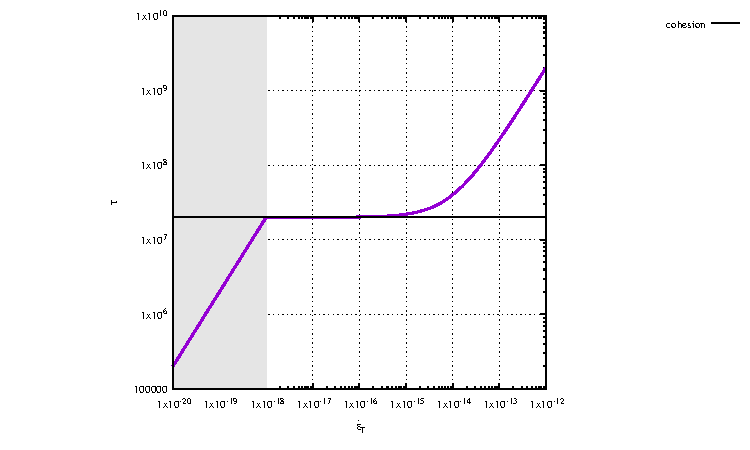
\includegraphics[width=5.5cm]{images/rheology/vvp/tau.pdf}
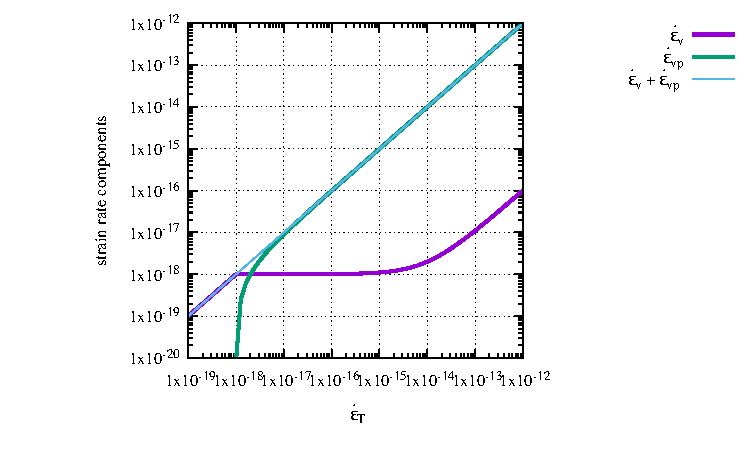
\includegraphics[width=5.5cm]{images/rheology/vvp/strainrates.pdf}
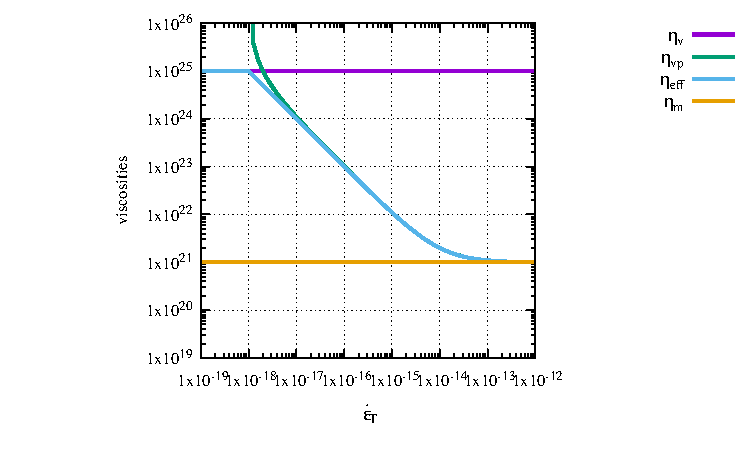
\includegraphics[width=5.5cm]{images/rheology/vvp/viscosities.pdf}\\
{\captionfont Obtained for $\eta_m=10^{21}$, $Y=20$MPa and $\eta_v=10^{25}$. Python code 
in images/rheology/vvp/}
\end{center}

In the following plots the resulting stress $\tau$ and effective viscosities $\eta_{eff}$
are compared between the above approach ('new') and the simpler (and naive) 
approach where $\dot\varepsilon_T$ 
is used in $\eta_{vp}$ instead of $\dot\varepsilon$ ('old'). In this particular case 
we see that it makes a difference at low strain rates close to the brittle-ductile transition.

\begin{center}
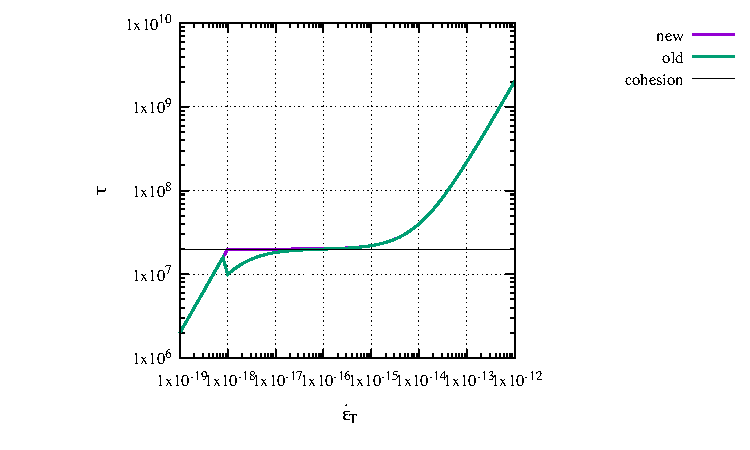
\includegraphics[width=8cm]{images/rheology/vvp/tau_comp.pdf}
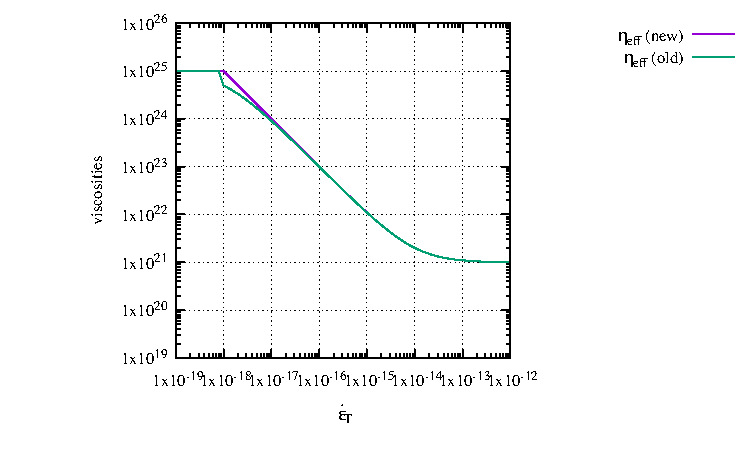
\includegraphics[width=8cm]{images/rheology/vvp/viscosities_comp.pdf}\\
{\captionfont Obtained for $\eta_m=10^{21}$, $Y=20$MPa and $\eta_v=10^{25}$. Python code 
in images/rheology/vvp/}
\end{center}

\begin{remark}
The introduction of the damper $\eta_m$ in parallel with the plastic element has an unavoidable
effect: the stress $\tau$ becomes larger than $Y$ at high strain rate values! Since the $vp$ 
block is akin to a bingham fluid, this is no surprise.
\end{remark}

\begin{remark}
The viscous dashpot $\eta_v$ also acts as a maximum viscosity cutoff: if $\eta_{vp}$ becomes (very) large, i.e. $\eta_{vp} \gg \eta_v$, then $\eta_{eff} \rightarrow \eta_v$.
Conversely, if $\eta_p=Y/2\dot\varepsilon_{vp}$ becomes (very) small, i.e. $\eta_p \ll \eta_m$ then $\eta_m$ acts as a minimum viscosity limiter, i.e. $\eta_{vp} \rightarrow \eta_m$. 
Since $\eta_m \ll \eta_v$ then $\eta_{eff} \rightarrow \eta_m$.
\end{remark}

\underline{A simple regularisation} This idea originates in Massmeyer \etal (2013) \cite{madd13}. We postulate
\[
\tilde{\eta}_{eff} = \left(  1 - \exp (- \frac{\dot\varepsilon_T}{\dot\varepsilon_{T}^c}) \right)
\left( \frac{Y}{2 \dot\varepsilon_T} + \eta_m \right)
\]
where $\dot\varepsilon_{T}^c$ is the critical strain  rate at which the transition viscous to 
viscous-viscoplastic occues given by $\dot\varepsilon_{T}^c=Y/2\eta_v$.
When $\dot\varepsilon_{T} \ll \dot\varepsilon_{T}^c$ then the exponential term tends to zero and 
\[
\tilde{\eta}_{eff} \rightarrow  \frac{Y}{2 \dot\varepsilon_T} + \eta_m 
\]
and if $\dot\varepsilon_{T} \rightarrow \infty$ then $\tilde{\eta}_{eff}\rightarrow \eta_m$.
Conversely if $\dot\varepsilon_T \rightarrow 0$ then we can carry out a Taylor expansion of the exponential 
term ($\exp x \sim 1 + x$ when $x$ is small).
\[
\tilde{\eta}_{eff} \sim \left(  \frac{\dot\varepsilon_T}{\dot\varepsilon_{T}^c} \right)
\left( \frac{Y}{2 \dot\varepsilon_T} + \eta_m \right)
\rightarrow 
\frac{\dot\varepsilon_T}{\dot\varepsilon_{T}^c}  \frac{Y}{2 \dot\varepsilon_T}  = \eta_v
\]
At low strain rates the viscosity does not 'explode' but actually converges to the background viscosity $\eta_v$.
The stress $\tau$ corresponding to this viscosity is simply $\tilde{\tau} = 2 \tilde{\eta}_{eff}$. 
Both $\tilde{\tau}$ and $ \tilde{\eta}_{eff}$ are plotted hereunder:


\begin{center}
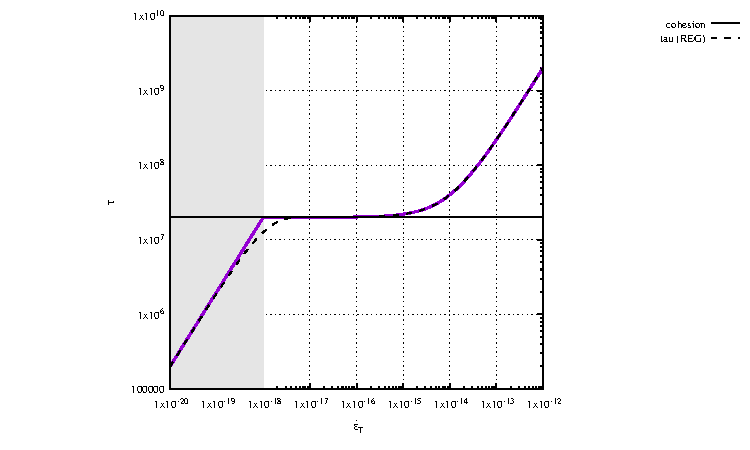
\includegraphics[width=7.5cm]{images/rheology/vvp/tau_reg.pdf}
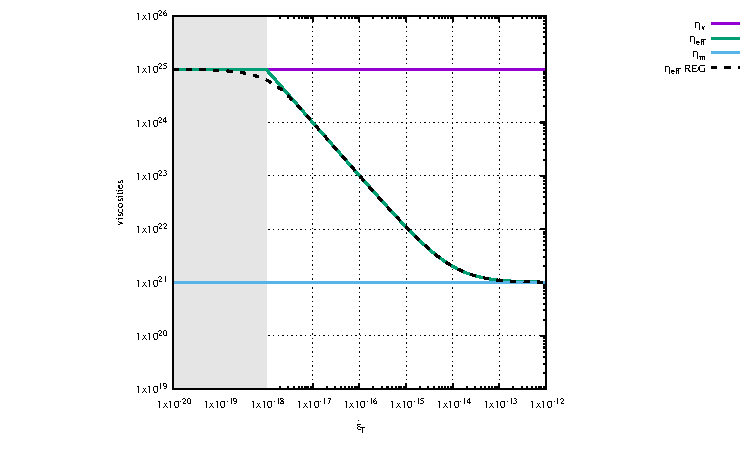
\includegraphics[width=7.5cm]{images/rheology/vvp/viscosities_reg.pdf}\\
{\captionfont Obtained for $\eta_m=10^{21}$, $Y=20$MPa and $\eta_v=10^{25}$. Python code 
in images/rheology/vvp/}
\end{center}


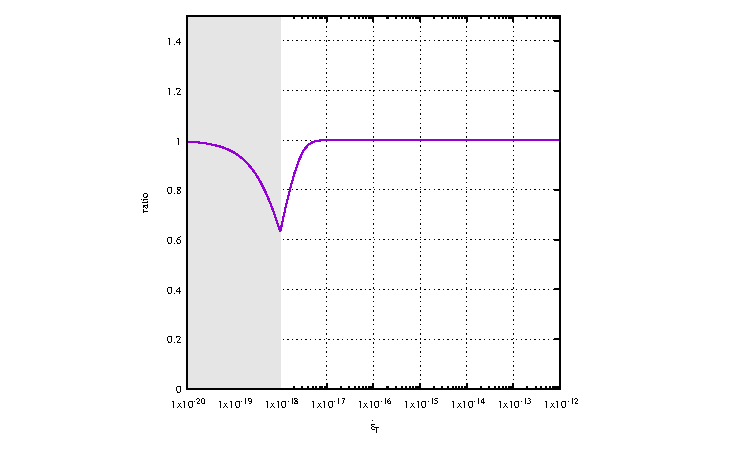
\includegraphics[width=7.5cm]{images/rheology/vvp/ratio_visc.pdf}



%which, if  yields the following effective viscosity:
%\[
%\eta_{eff} = \left( \frac{1}{\eta_M}  + \frac{1}{\frac{Y}{2 \dot{\varepsilon}_e} + \eta_m}  \right)^{-1}
%\]
%When the strain rate becomes very small,  $\dot{\varepsilon}_e \rightarrow 0$, $\eta_{eff}\rightarrow \eta_{M}$.
%When the strain rate becomes very large,  $\dot{\varepsilon}_e \rightarrow \infty$, $\eta_{eff}\rightarrow \eta_{m}$.
%We can then rewrite the above equation as a function of $\eta_{min}$ and $\eta_{max}$:
%\[
%\eta_{eff} = \left( \frac{1}{\eta_{max}}  + \frac{1}{\frac{c}{2 \dot{\varepsilon}_e} + \eta_{min}}  \right)^{-1}
%\]
%
%The effective viscosity is plotted here for various values of the minimum viscosity (for $c$=200MPa and $\eta_{max}=10^{25}Pa.s$:
%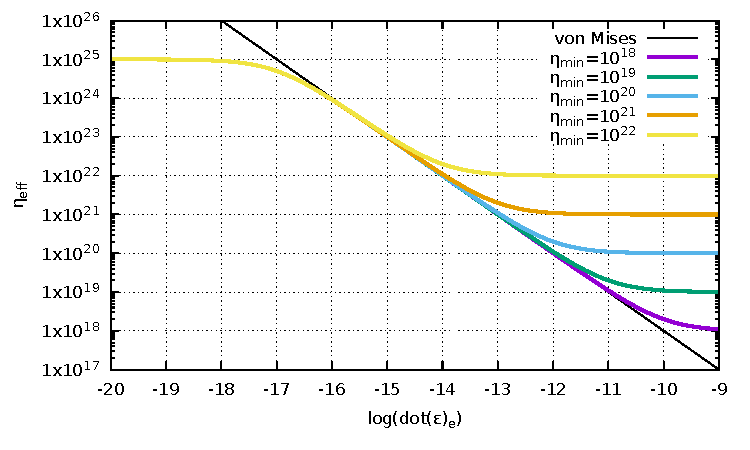
\includegraphics[width=8cm]{images/viscoplasticity/nu_eff}



\item \underline{two nonlinear viscous dampers in series:} 

\begin{center}
\begin{tikzpicture}
%\draw[fill=gray!23,gray!23](0,0) rectangle (6,4.5);
%\draw[step=0.5cm,gray,very thin] (0,0) grid (6,4.5); %background grid

%left wall
\node[] at (0.1,2.7) {$\tau$};
\draw[line width=1mm] (0.5,1.5) -- (0.5,3.5) ;   
\draw [->] (0,2.5) -- (0.45,2.5);
\draw [->] (0,2) -- (0.45,2);
\draw [->] (0,3) -- (0.45,3);

%dashpots
\draw[thick] (0.5,2.5) -- (2,2.5) ;   
\draw[thick] (2.5,2.5) -- (4,2.5) ;   
\draw[thick] (4.5,2.5) -- (5.5,2.5) ;   
\draw[thick] (1.5,3) -- (2.5,3) -- (2.5,2) -- (1.5,2);  
\draw[thick] (3.5,3) -- (4.5,3) -- (4.5,2) -- (3.5,2);  

\node[] at (2,1.5) {$\eta_{ds}$};
\node[] at (4,1.5) {$\eta_{dl}$};

%wall
\draw[line width=2mm] (5.5,1.5) -- (5.5,3.5) ;   
\draw[thick] (5.5,1.5)  -- (5.75,1.75) ;   
\draw[thick] (5.5,1.75) -- (5.75,2) ;   
\draw[thick] (5.5,2)    -- (5.75,2.25) ;   
\draw[thick] (5.5,2.25) -- (5.75,2.5) ;   
\draw[thick] (5.5,2.5)  -- (5.75,2.75) ;   
\draw[thick] (5.5,2.75) -- (5.75,3) ;   
\draw[thick] (5.5,3)    -- (5.75,3.25) ;   
\draw[thick] (5.5,3.25) -- (5.75,3.5) ;

\draw[>=triangle 45, <->] (0.5,0.95) -- (3.,0.95);
\draw[>=triangle 45, <->] (3.,0.95) -- (5.5,0.95);
\node[] at (2,0.65)   {$\dot\varepsilon_{ds}$};
\node[] at (4.25,0.65)   {$\dot\varepsilon_{dl}$};

\end{tikzpicture}

\end{center}

There are two dashpots in series, one accounts for dislocation creep, the other for diffusion creep.
The algorithm goes then as follows:
\begin{enumerate}
\item Assume we know $\dot\varepsilon_T$ (from previous iteration). 
\item The dashpots are in series so 
\[
\dot\varepsilon_T = \dot\varepsilon_{ds} + \dot\varepsilon_{df} 
\]
with
\begin{eqnarray}
\dot\varepsilon_{ds}  &=& A_{ds} \tau^n \exp \left(-\frac{Q_{ds}+pV_{ds}}{RT}\right) \label{sr_ds1} \\
\dot\varepsilon_{df}  &=& A_{df} \tau   \exp \left(-\frac{Q_{df}+pV_{df}}{RT}\right) \label{sr_df1} 
\end{eqnarray}
such that we are in fact looking for the stress value $\tau$ so that 
\[
\dot\varepsilon_T = 
A_{ds} \tau^n \exp \left(-\frac{Q_{ds}+p V_{ds}}{RT}\right) 
+
A_{df} \tau   \exp \left(-\frac{Q_{df}+p V_{df}}{RT}\right) 
\]
or, we must find the zero of the function ${\cal F}(\tau)$: 
\[
{\cal F}(\tau) =  \dot\varepsilon_T 
- A_{ds} \tau^n \exp \left(-\frac{Q_{ds}+p V_{ds}}{RT}\right) 
- A_{df} \tau   \exp \left(-\frac{Q_{df}+p V_{df}}{RT}\right) 
\]
This equation can be solved with a Newton-Raphson algorithm
and the iterations will be of the form:
\[
\tau_{n+1} = \tau_n - \frac{{\cal F}(\tau_n)}{{\cal F}'(\tau_n)}
\]
where the derivative of the function ${\cal F}$ with respect to $\tau$ reads:
\[
{\cal F}'(\tau)=\frac{\partial {\cal F}}{\partial \tau}=
- A_{ds} n \tau^{n-1} \exp\left(-\frac{Q_{ds}+pV_{ds}}{RT}\right)
- A_{df} \exp\left(-\frac{Q_{df}+pV_{df}}{RT}\right) 
\]
Once the value of $\tau$ is found, 
the strain rate values of Eqs. (\ref{sr_ds1}) and (\ref{sr_df1})
can be computed and so can the respective effective viscosities:
\begin{eqnarray}
\eta_{ds} 
&=& \frac{1}{2} A_{ds}^{1/n} \dot\varepsilon_{ds}^{\frac{1}{n}-1} \exp \left(\frac{Q_{ds}+pV_{ds}}{nRT}\right) \\
\eta_{df} 
&=& \frac{1}{2} A_{df}^{1/n}  \exp \left(\frac{Q_{df}+pV_{df}}{RT}\right) 
\end{eqnarray}
Their average effective viscosity $\tilde{\eta}_{eff}$ is given by 
\[
\tilde{\eta}_{eff} = \left( \frac{1}{\eta_{ds}} + \frac{1}{\eta_{df}} \right)^{-1}
\]
\end{enumerate}


Rather importantly, as we will see hereafter, the following variant is implemented 
in some codes (e.g. \douar, \fantom, \sopale, and probably many others) 
so as to bypass these costly Newton iterations:
\begin{enumerate}
\item compute $\eta_{ds}$ and $\eta_{df}$ with the {\it same} strainrate $\dot\varepsilon_T$, 
pressure and temperature values
\item average them by means of an harmonic average
\end{enumerate}
In this case, we have
\[
\dot{\varepsilon}_{\color{red} T}= 
A_{df} \tau_{df} \exp\left(-\frac{Q_{df}+pV_{df}}{RT}\right)
\quad\quad\quad
\dot{\varepsilon}_{\color{red} T}= 
A_{ds} \tau_{ds}^n \exp\left(-\frac{Q_{ds}+pV_{ds}}{RT}\right)
\]
or, 
\begin{eqnarray}
\eta_{ds} 
&=& \frac{1}{2} A_{ds}^{1/n} \dot\varepsilon_{\color{red}T}^{\frac{1}{n}-1} \exp \left(\frac{Q_{ds}+pV_{ds}}{nRT}\right) \\
\eta_{df} 
&=& \frac{1}{2} A_{df}^{1/n}  \exp \left(\frac{Q_{df}+pV_{df}}{RT}\right) 
\end{eqnarray}
We see that this simplification has consequences on the dislocation creep viscosity only.


\paragraph{A concrete example}
Let us consider a vertical section of upper mantle, from 660\si{\km} depth to 30\si{\km} depth.
The lithosphere is assumed to be 90\si{\km} thick. The temperature at the moho (the top
of the domain) is set to 550C, 1330C at the LMB and 1380C at the bottom.
A constant strainrate $\dot{\epsilon}_T=10^{-15}\si{\per\second}$ is assumed. 
We assume that the pressure is lithostatic (for simplicity 
the density is taken to be constant at 3300kg/m$^3$).
The temperature and pressure fields are shown hereunder:
\begin{center}
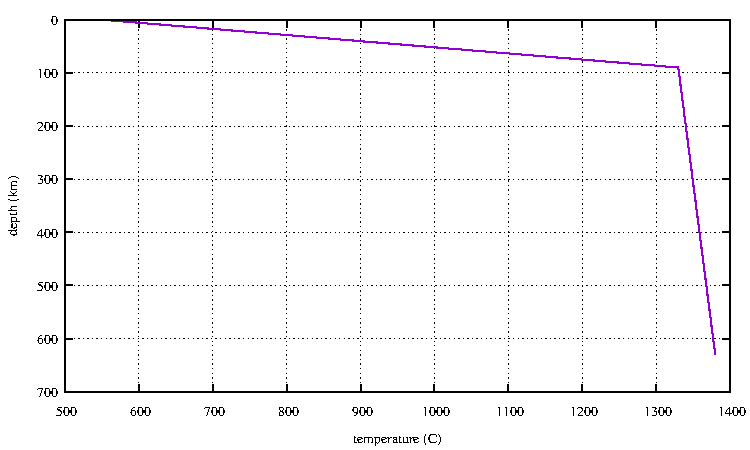
\includegraphics[width=6cm]{images/rheology/effvisc/temperature.pdf}
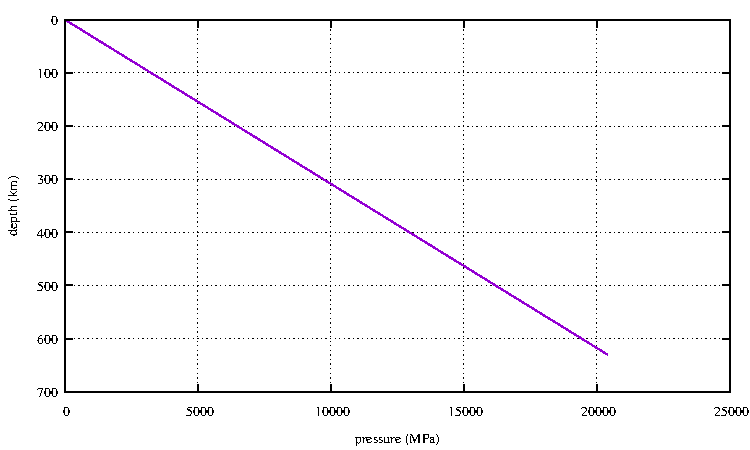
\includegraphics[width=6cm]{images/rheology/effvisc/pressure.pdf}
\end{center}

Material properties are taken from Karato \& Wu (1993) \cite{kawu93}.
The (fortran) code is available in {\tt images/rheology/effvisc/}.

In what follows, the values obtained with Newton iterations are coined 'NR'
and those obtained without are coined 'CHEAP'.
The diffusion and dislocation creep viscosities can be
computed for both algorithms and are shown hereunder
(As mentioned earlier the diffusion creep viscosity is independent of strain rate so
is the same for both):
\begin{center}
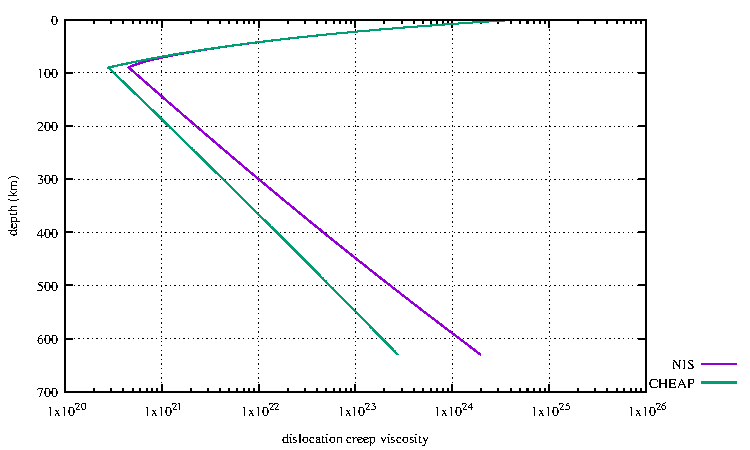
\includegraphics[width=6cm]{images/rheology/effvisc/both_mu_ds.pdf}
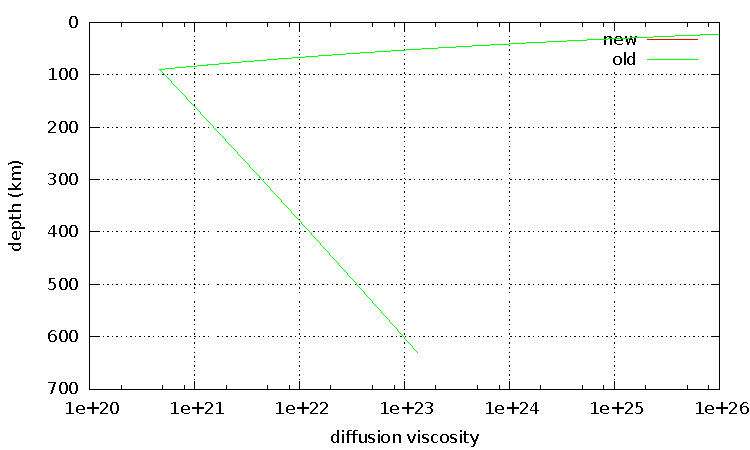
\includegraphics[width=6cm]{images/rheology/effvisc/both_mu_df.pdf}
\end{center}
We can also plot the resulting effective viscosity 
$\eta_{eff}$ for both approaches and we see that the differences 
are larger than 20\%. This is shown here under on the left, 
alongside with the partitioning of the strain rate as a function of depth:
\begin{center}
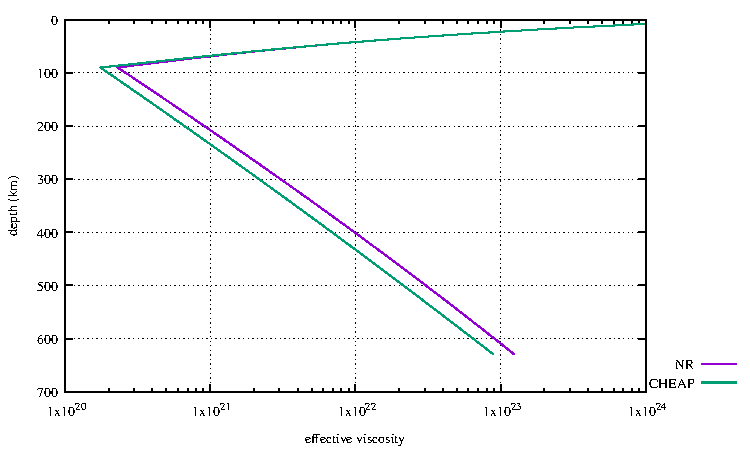
\includegraphics[width=8cm]{images/rheology/effvisc/both_mueff.pdf}
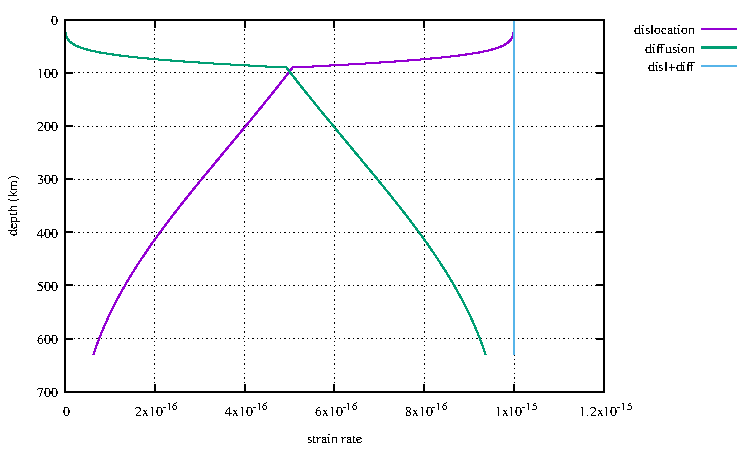
\includegraphics[width=8cm]{images/rheology/effvisc/both_sr.pdf}
\end{center}


























\item \underline{multiple viscous dampers and a plastic element} arranged as follows:



\begin{center}
\begin{flushright} {\tiny {\color{gray} (tikz\_vvp2.tex)}} \end{flushright}
%~~~~~~~~~~~~~~~~~~~~~~~~~~~~~~~~~~~~~~~~~~~~~~~~~~~~~~~~~~~~~~~~~~~~~~~~~~~~~~~~~~~~~~~~~~~~~~~~~~

\begin{center}
\begin{tikzpicture}
%\draw[fill=gray!23,gray!23](0,0) rectangle (7,5);
%\draw[step=0.5cm,gray,very thin] (0,0) grid (12,5); %background grid

\node[] at (0.1,2.7) {$\tau$};
\draw[line width=1mm] (0.5,1.5) -- (0.5,3.5) ;  
\draw [->] (0,2.5) -- (0.45,2.5);
\draw [->] (0,2) -- (0.45,2);
\draw [->] (0,3) -- (0.45,3);

%linear viscous

\draw[thick] (1.,3) -- (2.,3) -- (2.,2) -- (1.,2);  
\draw[thick] (0.5,2.5) -- (1.5,2.5) ;  
\draw[>=triangle 45, <->] (0.5,0.95) -- (2.5,0.95);
\node[] at (1.7,0.75) {$\dot\varepsilon_{v}$};
\node[] at (1.5,1.6) {$\eta_{m}$};


%dislocation creep
\draw[thick] (2.,2.5) -- (4,2.5) ;  
\draw[thick] (4.5,2.5) -- (6.5,2.5) ;  
\draw[thick] (3.5,3) -- (4.5,3) -- (4.5,2) -- (3.5,2);  
\node[] at (4,1.6) {$\eta_{ds}$};
\draw[>=triangle 45, <->] (2.5,0.95) -- (5,0.95);
\node[] at (4,0.75)   {$\dot\varepsilon_{ds}$};

%diffusion creep
\draw[thick] (6.,3) -- (7.,3) -- (7.,2) -- (6.,2);  
\node[] at (6.5,1.6) {$\eta_{df}$};
\draw[thick] (7,2.5) -- (8.5,2.5) ;  
\draw[>=triangle 45, <->] (5,0.95) -- (7.5,0.95);
\node[] at (6.5,0.75)   {$\dot\varepsilon_{df}$};

%viscoplastic element
\draw[thick] (9.5,4) -- (10.5,4) -- (10.5,3) -- (9.5,3);  
\node[] at (10,4.3) {$\eta_m$};
\node[] at (10,1.9) {$Y$};
\draw[thick] (10,3.5) -- (8.5,3.5) -- (8.5,1.5) -- (9,1.5);  
\draw[thick] (10.5,3.5) -- (11.5,3.5) -- (11.5,1.5) -- (11,1.5);  
\draw[thick] (9,1.5) -- (9.5,1.4) -- (10.5,1.4) ;  
\draw[thick] (9.5,1.6) -- (10.5,1.6) -- (11,1.5) ;  
\draw[thick] (11.5,2.5) -- (13,2.5) ;  
\draw[>=triangle 45, <->] (7.5,0.95) -- (13,0.95);
\node[] at (10.2,0.75) {$\dot\varepsilon_{vp}$};

%wall
\draw[line width=2mm] (13,1.5) -- (13,3.5) ;  
\draw[thick] (13,1.5)  -- (13.25,1.75) ;  
\draw[thick] (13,1.75) -- (13.25,2) ;  
\draw[thick] (13,2)    -- (13.25,2.25) ;  
\draw[thick] (13,2.25) -- (13.25,2.5) ;  
\draw[thick] (13,2.5)  -- (13.25,2.75) ;  
\draw[thick] (13,2.75) -- (13.25,3) ;  
\draw[thick] (13,3)    -- (13.25,3.25) ;  
\draw[thick] (13,3.25) -- (13.25,3.5) ;  





\end{tikzpicture}\\
\end{center}

\end{center}



The algorithm goes then as follows:
\begin{enumerate}
\item Assume we know $\dot\varepsilon_T$ (from previous iteration), 
as well as the plasticity parameters $Y$ (a constant in the case of von Mises, or a pressure-dependent 
quantity otherwise) and $\eta_m$.
\item We start by assuming that the plasticity 'block' is not active ($\dot{\varepsilon}_{vp}=0$): we have then three dampers in series. 
We need their associated strain rates 
$\dot{\varepsilon}_{df}$ and $\dot{\varepsilon}_{ds}$ which are such that 
\[
\dot\varepsilon_T = 
\dot\varepsilon_v + \dot\varepsilon_{ds} + \dot\varepsilon_{df} 
\]
with
\begin{eqnarray}
\dot\varepsilon_v &=& \frac{\tau}{2 \eta_v} \label{sr_v} \\
\dot\varepsilon_{ds}  &=& A_{ds} \tau^n \exp \left(-\frac{Q_{ds}+pV_{ds}}{RT}\right) \label{sr_ds} \\
\dot\varepsilon_{df}  &=& A_{df} \tau   \exp \left(-\frac{Q_{df}+pV_{df}}{RT}\right) \label{sr_df} 
\end{eqnarray}
such that we are in fact looking for the stress value $\tau$ so that 
\[
\dot\varepsilon_T = 
A_{ds} \tau^n \exp \left(-\frac{Q_{ds}+p V_{ds}}{RT}\right) 
+
A_{df} \tau   \exp \left(-\frac{Q_{df}+p V_{df}}{RT}\right) 
+
\frac{\tau}{2 \eta_v}
\]
or, we must find the zero of the function ${\cal F}$: 
\[
{\cal F}(\tau) = 
\dot\varepsilon_T 
- A_{ds} \tau^n \exp \left(-\frac{Q_{ds}+p V_{ds}}{RT}\right) 
- A_{df} \tau   \exp \left(-\frac{Q_{df}+p V_{df}}{RT}\right) 
- \frac{\tau}{2 \eta_v} 
\]
This equation can be solved with a Newton-Raphson algorithm
and the iterations will be of the form:
\[
\tau_{n+1} = \tau_n - \frac{{\cal F}(\tau_n)}{{\cal F}'(\tau_n)}
\]
where the derivative of the function ${\cal F}$ with respect to $\tau$ reads:
\[
{\cal F}'(\tau)=\frac{\partial {\cal F}}{\partial \tau}=
- A_{df} \exp\left(-\frac{Q_{df}+pV_{df}}{RT}\right) 
- A_{ds} n \tau^{n-1} \exp\left(-\frac{Q_{ds}+pV_{ds}}{RT}\right)
- \frac{1}{2\eta_v}
\]
Once the value of $\tau$ is found, 
the strain rate values of Eqs. (\ref{sr_ds}), (\ref{sr_df}) and (\ref{sr_v}) 
can be computed and so can the respective effective viscosities:
\begin{eqnarray}
\eta_{ds} 
&=& \frac{1}{2} A_{ds}^{1/n} \dot\varepsilon_{ds}^{\frac{1}{n}-1} \exp \left(\frac{Q_{ds}+pV_{ds}}{nRT}\right) \\
\eta_{df} 
&=& \frac{1}{2} A_{df}^{1/n}  \exp \left(\frac{Q_{df}+pV_{df}}{RT}\right) 
\end{eqnarray}
Their average effective viscosity $\tilde{\eta}_{eff}$ is given by 
\[
\tilde{\eta}_{eff} = \left( \frac{1}{\eta_{ds}} + \frac{1}{\eta_{df}} + \frac{1}{\eta_v} \right)^{-1}
\]


\item if $\tau =2 \tilde{\eta}_{eff} \dot\varepsilon_T < Y$ the stress is below the yield stress value 
and the plasticity element is indeed not active. Use $\tilde{\eta}_{eff}$ in the material model.

\item if $\tau=2 \tilde{\eta}_{eff} \dot\varepsilon_T > Y$ the stress is above the yield value, which is not 
allowed. In this case the plastic element must be present and active and the viscous dampers are then 
in series with the (visco)plastic element. The formers deform 
with a strain rate $\dot{\varepsilon}_v$, $\dot\epsilon_{ds}$ and $\dot{\epsilon}_{df}$ 
while the latter with $\dot\epsilon_{vp}$ (all under the same tress $\tau$) 
and we have  $\dot\varepsilon_T = \dot{\varepsilon}_v + \dot\varepsilon_{ds} + \dot\varepsilon_{df} + \dot\varepsilon_{vp}$ so:

\begin{eqnarray}
\dot\varepsilon_T - \dot{\varepsilon}_v(\tau) - \dot\varepsilon_{ds}(\tau) - \dot\varepsilon_{df}(\tau)  
&=& \dot\varepsilon_{vp}  \nonumber\\
&=& \frac{\tau}{2 \left( \frac{Y}{2\dot\varepsilon_{vp}} + \eta_m  \right)} 
\nonumber\\
%&=&  \frac{\tau}{2 \left( \frac{Y}{2 (\dot\varepsilon_T -\dot{\varepsilon}_v(\tau) -\dot\varepsilon_{ds}(\tau) 
%+ \dot\varepsilon_{df}(\tau)   )} + \eta_m  \right)} 
%\nonumber\\
\dot\varepsilon_T -  \dot{\varepsilon}_v(\tau) -\dot\varepsilon_{ds}(\tau) - \dot\varepsilon_{df}(\tau) 
&=&
\frac{\tau}{2 \left( \frac{Y}{2 (\dot\varepsilon_T -\dot{\varepsilon}_v(\tau) -\dot\varepsilon_{ds}(\tau) 
+ \dot\varepsilon_{df}(\tau)   )} + \eta_m  \right)} \nonumber
\\
2 [\dot\varepsilon_T -\dot{\varepsilon}_v(\tau) -\dot\varepsilon_{ds}(\tau) - \dot\varepsilon_{df}(\tau) ]
 \left( \frac{Y}{2 (\dot\varepsilon_T -\dot{\varepsilon}_v(\tau) -\dot\varepsilon_{ds}(\tau) + \dot\varepsilon_{df}(\tau)   )} + \eta_m  \right) &=& \tau 
\nonumber\\
Y + 2 (\dot\varepsilon_T - \dot{\varepsilon}_v(\tau) -\dot\varepsilon_{ds}(\tau) - \dot\varepsilon_{df}(\tau) ) \eta_m  &=& \tau \nonumber 
\end{eqnarray}
As before, we must find the zero of the function ${\cal F}$: 
\begin{eqnarray}
{\cal F}(\tau) 
&=& Y + 2 [\dot\varepsilon_T -\dot{\varepsilon}_v(\tau)- \dot\varepsilon_{ds}(\tau) -\dot\varepsilon_{df}(\tau) ]\eta_m -\tau \nonumber\\
&=& Y + 2 \left[ 
\dot\varepsilon_T - \frac{\tau}{2\eta_v}-A_{ds} \tau^n \exp \left(-\frac{Q_{ds}+pV_{ds}}{RT}\right) 
- A_{df} \tau   \exp \left(-\frac{Q_{df}+pV_{df}}{RT}\right)  
\right]\eta_m -\tau \nn
\end{eqnarray}
Because dislocation creep involves the $n$-th power of the stress we will here also need 
to find the zero by means of a Newton-Raphson algorithm. 

We have:
\begin{eqnarray}
\frac{\partial {\cal F}}{\partial \tau} &=&
\left[
- \frac{1}{\eta_v} 
-2 \frac{\partial  \dot\varepsilon_{ds}(\tau) }{\partial \tau} 
-2 \frac{\partial  \dot\varepsilon_{df}(\tau) }{\partial \tau} 
\right] \eta_m - 1
\end{eqnarray}

\begin{eqnarray}
{\cal F}(\tau) / 2\eta_m 
&=& 
\frac{Y}{2\eta_m}  + \dot\varepsilon_T 
- \frac{\tau}{2\eta_v}
- A_{ds}(p,T) \tau^n 
- A_{df}(p,T) \tau  
- \frac{\tau}{2\eta_m} \\
&=& 
- A_{ds}(p,T) \tau^n - \left(A_{df}(p,T) +  \frac{1}{2\eta_v} -\frac{1}{2\eta_m} \right) \tau
+ 
\left( \frac{Y}{2\eta_m}  + \dot\varepsilon_T \right) =0
\end{eqnarray}



\end{enumerate}

Note that when $\eta_m=0$ we logically recover $\tau=Y$ as the stress cannot exceed the yield strength $Y$.

Although this approach is probably the most consistent in terms of physics, the presence 
of the Newton-Raphson iterations makes it very expensive since this procedure is to be repeated 
for every quadrature point or every particle.

Let us consider a concrete example: we set $Y=20\si{\mega\pascal}$, $\eta_v=10^{25}\si{pascal}$, 
$\eta_m=10^{20}\si{pascal}$. The domain is one-dimensional of depth $660\si{km}$. The density is
assumed to be constant at $3300\si{\kg\per\cubic\metre}$. Dislocation and diffusion creep parameters
are taken from Karato \& Wu (1993) \cite{kawu93}. The temperature is linear is $20\si{\celsius}$ 
at the surface, $550\si{\celsius}$ at $30\si{km}$ depth, $1330\si{celsius}$ at $90\si{\km}$ depth 
and $1380\si{\celsius}$ at the bottom. Pressure is assumed to be lithostatic. 
The python program and the gnuplot script are in {\sl images/rheology/example}.

In the code I consider two cases: 'old' and 'new'. The latter is described above. 
'old' goes as follows: loop over total strain rate values. 
Compute dislocation and diffusion creep viscosities with it. Compute harmonic 
average of these with linear viscosity. Compute deviatoric stress value. 
use it in dislocation and diffusion formulae to arrive at respective strainrates. 

\newpage
\begin{center}
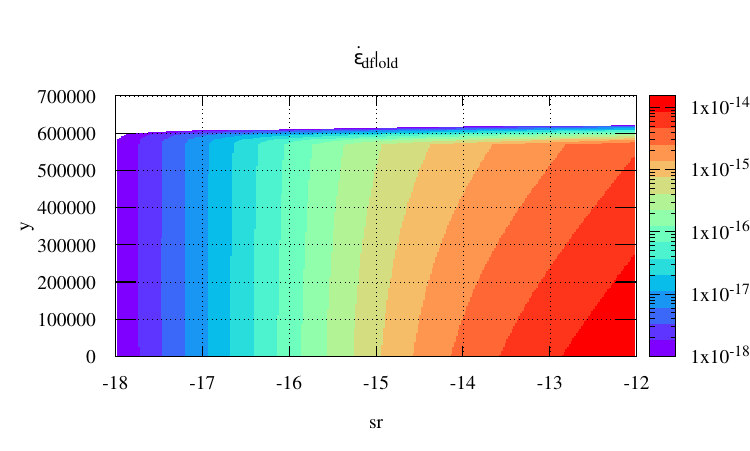
\includegraphics[width=5.5cm]{images/rheology/example/map_sr_df_old-1}
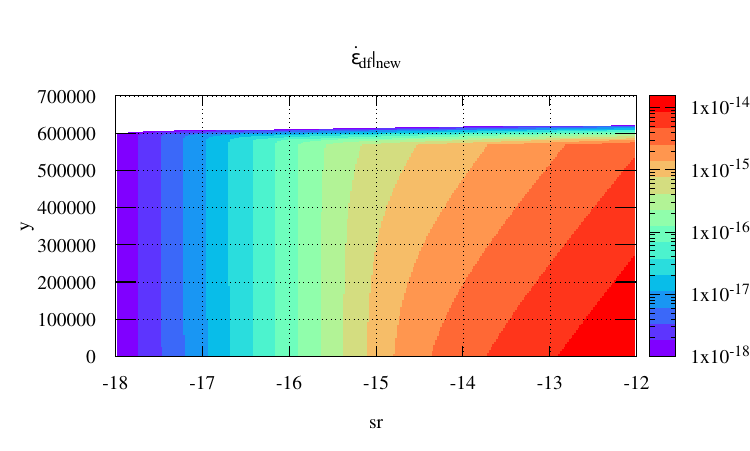
\includegraphics[width=5.5cm]{images/rheology/example/map_sr_df_new-1}
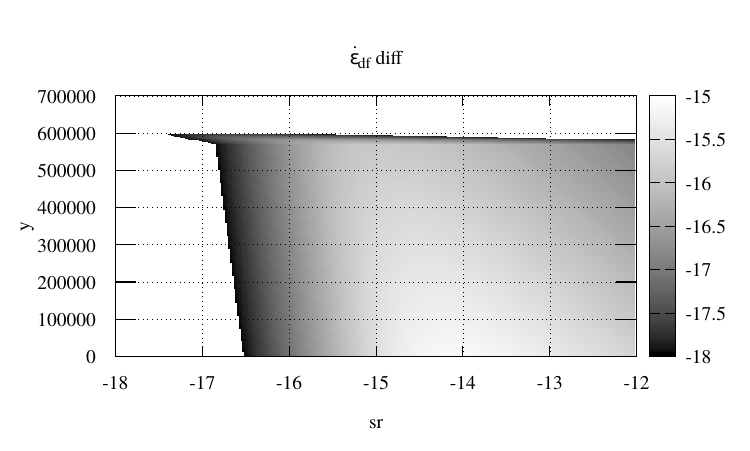
\includegraphics[width=5.5cm]{images/rheology/example/map_sr_df_diff-1}\\
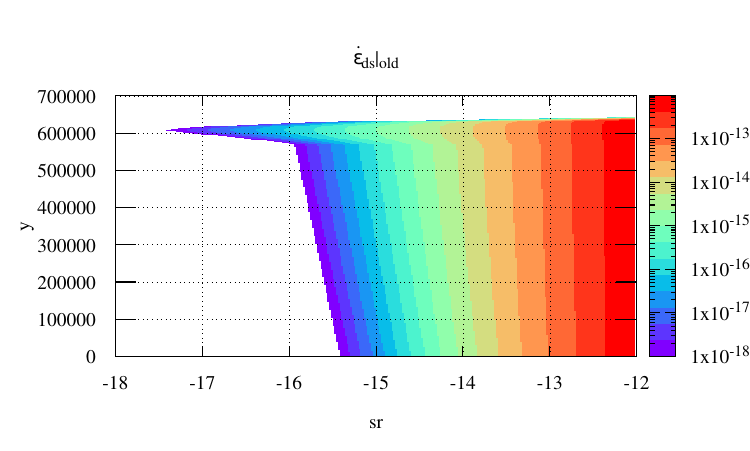
\includegraphics[width=5.5cm]{images/rheology/example/map_sr_ds_old-1}
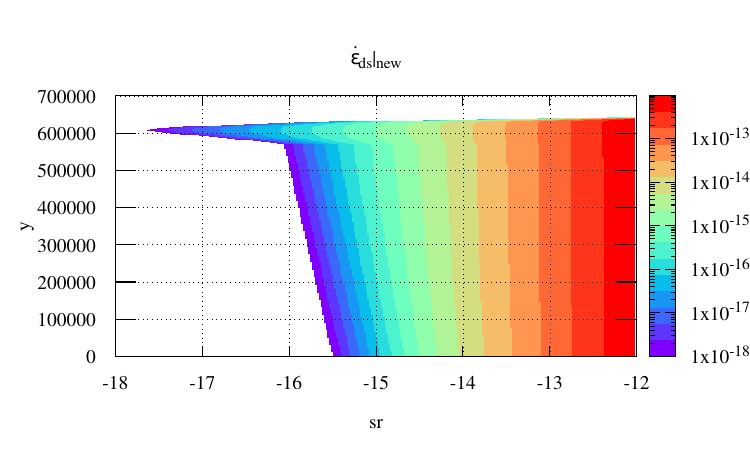
\includegraphics[width=5.5cm]{images/rheology/example/map_sr_ds_new-1}
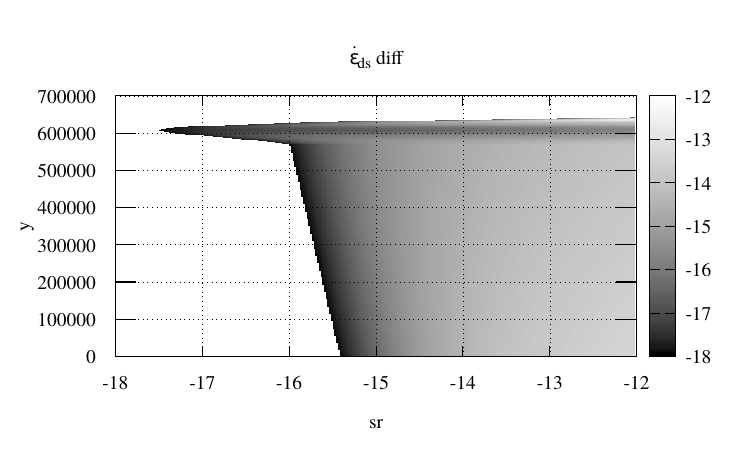
\includegraphics[width=5.5cm]{images/rheology/example/map_sr_ds_diff-1}\\
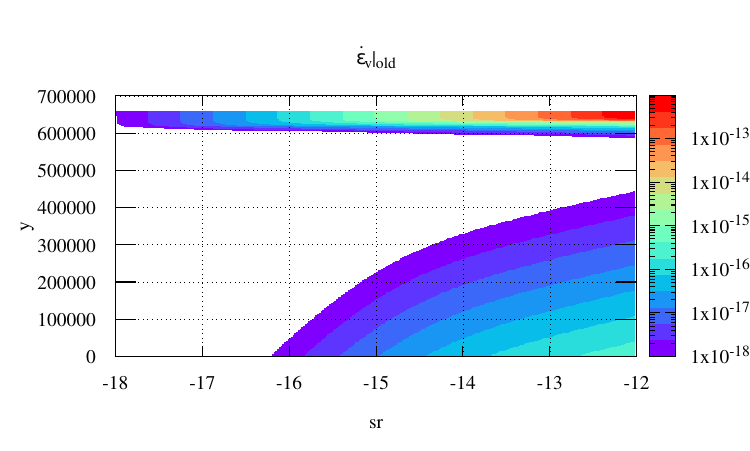
\includegraphics[width=5.5cm]{images/rheology/example/map_sr_v_old-1}
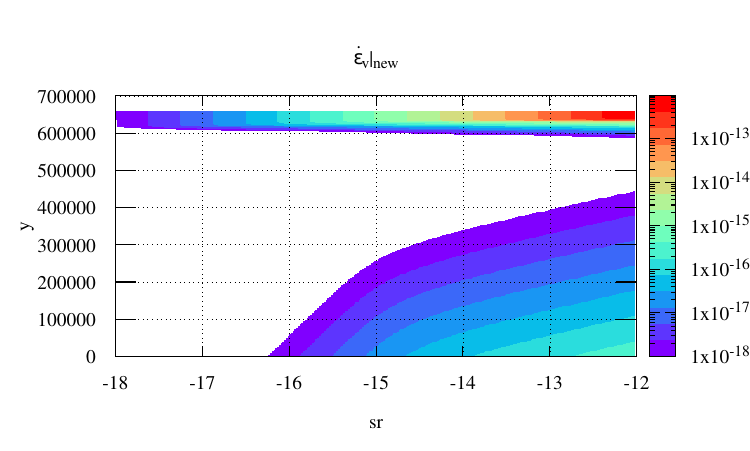
\includegraphics[width=5.5cm]{images/rheology/example/map_sr_v_new-1}
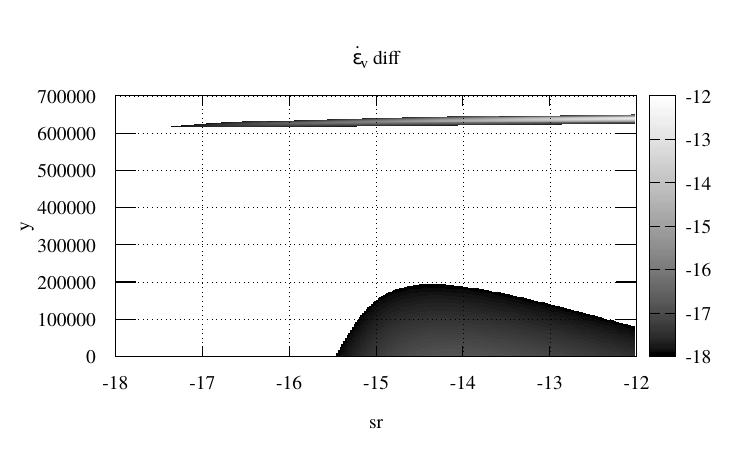
\includegraphics[width=5.5cm]{images/rheology/example/map_sr_v_diff-1}\\
\includegraphics[width=5.5cm]{images/rheology/example/map_etaeff_old-1}
\includegraphics[width=5.5cm]{images/rheology/example/map_etaeff_new-1}
\includegraphics[width=5.5cm]{images/rheology/example/map_etaeff_diff-1}\\
\includegraphics[width=5.5cm]{images/rheology/example/map_tau_old-1}
\includegraphics[width=5.5cm]{images/rheology/example/map_tau_new-1}
\includegraphics[width=5.5cm]{images/rheology/example/map_tau_diff-1}\\
\includegraphics[width=5.5cm]{images/rheology/example/profile_sr-1}
\includegraphics[width=5.5cm]{images/rheology/example/profile_tau-1}
\includegraphics[width=5.5cm]{images/rheology/example/profile_etaeff-1}\\
\includegraphics[width=5.5cm]{images/rheology/example/map_isplast_old-1}
\includegraphics[width=5.5cm]{images/rheology/example/map_isplast_new-1}\\
{\captionfont Viscous branch: (ds+df+v) 'old' stands 
for the old approach when $\dot{\varepsilon}_T$
was used for all mechanisms. 'new' stands for the new approach and the right strain rate 
decomposition.}
\end{center}



\newpage
\begin{center}
\includegraphics[width=5.5cm]{images/rheology/example/map_etaeff_old_pl-1}
\includegraphics[width=5.5cm]{images/rheology/example/map_etaeff_new_pl-1}
\includegraphics[width=5.5cm]{images/rheology/example/map_etaeff_diff_pl-1}\\
\includegraphics[width=5.5cm]{images/rheology/example/map_tau_old_pl-1}
\includegraphics[width=5.5cm]{images/rheology/example/map_tau_new_pl-1}
\includegraphics[width=5.5cm]{images/rheology/example/map_tau_diff_pl-1}\\
\includegraphics[width=5.5cm]{images/rheology/example/profile_sr_pl-1}
\includegraphics[width=5.5cm]{images/rheology/example/profile_tau_pl-1}
\includegraphics[width=5.5cm]{images/rheology/example/profile_etaeff_pl-1}\\
{\captionfont Visco-viscoplastic rheology: (ds+df+v+vp)} 
\end{center}




\end{itemize}




\begin{remark}
Chenin \etal (2019) \cite{chmd19}, 
base their rheological model on the additive decomposition of the following
deviatoric strain rate tensor ${\bm \varepsilon}^d$:
\[
{\bm \varepsilon}^d =
{\bm \varepsilon}^{el}+
{\bm \varepsilon}^{pl}+
{\bm \varepsilon}^{ds}+
{\bm \varepsilon}^{df}+
{\bm \varepsilon}^{pe}
\]
where the five strain rate terms correspond respectively to the elastic, plastic, 
and viscous creep (dislocation, diffusion, peierls) contributions. 
This implies that all these elements are in series and the associated 
viscosities are then averaged with an harmonic mean. 
Rather interestingly, it is then stated that "this strain rate equation is nonlinear
and solved locally on cell centroids and vertices in order to define the current effective viscosity 
and stress \cite{poso08}."
\end{remark}

\Literature: \cite{hoor89,lopr90,homo90,scps01,lova01,anpa19,elga10}


































%...........................................
\subsubsection{Anisotropic viscosity}

Following the paper by Lev and Hager (2008) \cite{leha08}, 
the anisotropic viscosity enters the equation of momentum through a 'correction'
term added to the isotropic part of the constitutive equation relating
stress and strain rate \cite{mumh02}:
\[
\sigma_{ij} = -p \delta_{ij} + 2 \eta_N \dot{\varepsilon}_{ij}  - 2(\eta_N-\eta_S)\Lambda_{ijkl}\dot{\varepsilon}_{kl} 
\]
where $\eta_N$ is the normal viscosity and $\eta_S$ is the shear viscosity. 
The fourth order tensor $\Lambda$ reflects the orientation of the directors in space, 
denoted by $\vec{n}$:
\[
\Lambda_{ijkl}=\frac{1}{2} (n_i n_k \delta_{lj} + n_j n_k \delta_{il} 
+ n_i n_l \delta_{kj} n_j n_l \delta_{ik} )
- 2 n_i n_j n_k n_l 
\]
Following \cite{modm03,mumh02}, the 'directors' are advected through the model and are 
analogous to particles. The directors are
vector-particles pointing normal to the easy-glide plane or layer,
thus defining the directions associated with $\eta_N$ and $\eta_S$. 
In each time step of the calculation, the directors are advected and rotated by the
flow, and in return determine the viscosity structure for the next time
step \cite{mumc04}.

\begin{center}
\includegraphics[width=10cm]{images/rheology/leha08}\\
{\captionfont Taken from Lev \& Hager (2008) \cite{leha08}.}
\end{center}

\mscthesis\index{general}{MSc Thesis}: redo the Rayleigh-Taylor instabilities with 
anisotropic lithospheric viscosity.
experiments of Lev \& Hager (2008) \cite{leha08}. Look at the three methods 
listed in the other article by 
Lev \& Hager \cite{leha08b}. 
Check Appendix B.2.2 or \cite{perr19} for additional results.

\Literature: 
Richter \& Daly (1978) \cite{rida78},
Saito \& Abe (1984) \cite{saab84},
Vauchez \etal (1998) \cite{vatb98},
M{\"u}lhaus \etal (2002) \cite{mumh02},
M{\"u}lhaus \etal (2003) \cite{mumc03},
M{\"u}lhaus \etal (2004) \cite{mumc04},
Michibayashi \& D. Mainprice (2004) \cite{mima04},
Moresi \& M{\"u}lhaus (2006) \cite{momu06},
M{\"u}lhaus \etal (2010) \cite{mumg10},
M{\"u}lhaus \etal (2011) \cite{muso11},
Sharples \etal (2016) \cite{shmv16},
Perry-Houts \& Karlstrom \cite{peka18},
Kiraly \etal (2020) \cite{kich20}

%...........................................
\subsubsection{Rheology of the lithosphere}

\begin{center}
\includegraphics[height=5cm]{images/rheology/budr08}\\
{\captionfont Schematic view of the three most common first order rheological models of the continental 
lithosphere under a strain rate of 10$^{-14}$s$^{-1}$ . 
In all three models the upper crust has its frictional strength increased with pressure and depth. 
(a) The jelly sandwich model has a weak mid-lower crust and a strong mantle composed of dry olivine. 
(b) The cr\`eme br\^ul\'ee model assumes that the mantle is weak, due to the presence of water and high 
temperature deformation, and the dry and brittle crust determines the strength of the lithosphere. 
(c) The banana split model assumes that the lithosphere as a whole has its strength greatly reduced
due to various strain weakening and feedback processes \cite{budr08}}
\end{center}

\begin{center}
\includegraphics[width=8cm]{images/rheology/bird99}\\
{\captionfont Taken from \cite{bird99}.
Typical vertical distribution of maximum shear stress in continental lithosphere 
undergoing compressional (right) or extensional (left) strain at $10^{-15}$s. 
Friction controls level of shear stress in upper part of crust and sometimes in mantle lithosphere;
then, below brittle/ductile transition, shear stress is controlled by thermally-activated dislocation creep.}
\end{center}

Molnar \cite{moln92} discusses the validity of the Brace-Goetze strength profiles. 
In particular, he has this to say about the power law parameters:
{\it
The uncertainty alone in $Q$ alone renders calculated strengths 
uncertain by 10 times at temperatures of about 700C.
Correspondingly, that uncertainty in Q is approximately equivalent 
to an uncertainty of about 100C in temperature.
}


\begin{center}
\begin{tabular}{l|l}
\hline

Wet Quartzite & upper crust  \cite{jahu12,wabj08} \\
              & upper continental crust \cite{kecw09,cube11} \\
              & lower crust  \cite{jahu12,wabj08} \\
              & ocean sediment \cite{kecw09} \\
Dry Olivine   & lithosphere  \cite{hube07}\\
              & sublithospheric mantle \cite{hube07}\\
Dry Maryland Diabase & lower crust \cite{wabj08,wabj08b} \\
                     & lower continental crust \cite{kecw09,cube11} \\
                     & oceanic crust \cite{wabj08,kecw09,wabj08b,cube11} \\
Wet Olivine   & continental mantle lithosphere \cite{wabj08,wabj08b} \\
              & oceanic mantle lithosphere \cite{wabj08,wabj08b} \\
              & sublithospheric mantle \cite{wabj08,kecw09,wabj08b} \\
              & mantle lithosphere \cite{kecw09} \\
\hline
\end{tabular}
\end{center}



\Literature \cite{buwa06,budr08,rana97a,rana97b}





\todo[inline]{I need to talk about Byerlee's law. \cite{byer78}}

